\documentclass[aps,prd,amsmath,floatfix
%,galley
,twocolumn
,superscriptaddress,nofootinbib,showpacs]{revtex4-1}

\usepackage{graphicx} %\usepackage{amsmath,amssymb}
\usepackage{amsfonts} \usepackage{subfigure} \usepackage{xspace}
\usepackage[usenames,dvipsnames]{color} \usepackage{dcolumn}
\usepackage{bm} \usepackage{hyperref} \usepackage{mathrsfs}
\usepackage[]{amsmath,amssymb} \usepackage[]{amsthm}
\usepackage{verbatim} \usepackage{appendix}
\usepackage[colorinlistoftodos]{todonotes}
%\usepackage[margin=0.75in]{geometry}

\theoremstyle{plain} \newtheorem{thm}{Theorem} \newtheorem{lem}{Lemma}
\newtheorem{prop}{Proposition} \theoremstyle{definition}
\newtheorem{defn}{Definition} \newcommand{\norm}[1]{\lVert#1\rVert} %
%This is for strikeout font
\usepackage{ulem} \normalem % end strikeout
%font

\newcommand{\red}[1]{\textcolor{Red}{#1}}
\newcommand{\cyan}[1]{\textcolor{Cyan}{#1}}
\newcommand{\green}[1]{\textcolor{Green}{#1}}
\newcommand{\magenta}[1]{\textcolor{Magenta}{#1}}
\newcommand{\note}[1]{\textcolor{Red}{[#1]}}
\newcommand{\subnote}[1]{\textcolor{Blue}{#1}}
\newcommand{\needcite}{\note{NEED CITATION}} %
\newcommand{\sascha}[1]{\textcolor{blue}{\textit{Sascha: #1}}} %
\newcommand{\mdh}[1]{\textcolor{cyan}{\textit{Mark: #1}}}
\newcommand{\harald}[1]{{\textcolor{OliveGreen}{#1}}} %
\newcommand{\larne}[1]{\textcolor{DarkOrchid}{[\textit{Larne: #1}]}}
\newcommand{\nick}[1]{\textcolor{blue}{\textit{Nick: #1}}}
\newcommand{\roland}[1]{\textcolor{Magenta}{\textit{ROLAND: #1}}}

%%% for \sout, to strike out text that has been replaced by an
%%% improved alternative.  \usepackage{ulem} \normalem

% Automatically deal with the author-list superscripts
%\usepackage{superscriptaddress}

\begin{document}



\title[Binary Neutron Stars with Arbitrary Spins in Numerical
  Relativity]{Binary Neutron Stars with Arbitrary Spins in Numerical
  Relativity}

\newcommand{\AEI}{\affiliation{Max Planck Institute for Gravitational Physics
(Albert Einstein Institute), Am M\"uhlenberg 1, Potsdam-Golm, 14476, Germany}} %
\newcommand{\Caltech}{\affiliation{Theoretical Astrophysics 350-17,
    California Institute of Technology, Pasadena, CA 91125, USA}}
\newcommand{\CITA}{\address{Canadian Institute for Theoretical
    Astrophysics, University of Toronto, 60~St.~George Street,
    Toronto, Ontario M5S 3H8, Canada}} %
\newcommand{\CIFAR}{\affiliation{Canadian Institute for Advanced
    Research, 180 Dundas St.~West, Toronto, ON M5G 1Z8, Canada}} %
\newcommand{\Cornell}{\affiliation{Center for Radiophysics and Space
    Research, Cornell University, Ithaca, New York 14853, USA}}
\newcommand{\DAA}{\affiliation{Department of Astronomy and
    Astrophysics, 50 St.\ George Street, University of Toronto,
    Toronto, ON M5S 3H4, Canada}}
\newcommand{\LBL}{\affiliation{Lawrence Berkeley National Laboratory,
    1 Cyclotron Rd, Berkeley, CA 94720, USA; Einstein Fellow}}
\newcommand{\WSU}{\affiliation{
Department of Physics \& Astronomy, Washington State University, Pullman, Washington 99164, USA}}
\author{Nick Tacik}\CITA\DAA
\author{Francois Foucart}\CITA\LBL
\author{Harald P. Pfeiffer}\CITA\CIFAR
\author{Roland Haas}\Caltech\AEI
\author{Jeff Kaplan}\Caltech
\author{Curran Muhlberger}\Cornell
\author{Matt Duez}\WSU
\author{Lawrence E. Kidder}\Cornell
\author{Mark A. Scheel}\Caltech
\author{B\'{e}la Szil\'{a}gyi}\Caltech


\begin{abstract}
  We present a code to construct initial data for binary neutron star
  where the stars are rotating.  Our code, based on the formalism
  developed by Tichy, allows for arbitrary rotation axes of the
  neutron stars and is able to achieve rotation rates near rotational
  breakup\harald{, as measured through quasi-local angular momentum
    integrals.  Preliminary evolutions show that the magnitude of the
    stars' angular momentum is conserved, and that the spin- and
    orbit-precession of the stars is well described by
    post-Newtonian approximation.}  We demonstrate that orbital
  eccentricity of the binary neutron stars can be controlled to
  $\sim 0.1\%$.  The neutron stars show
    quasi-normal mode oscillations at an amplitude which increases
    with the rotation rate of the stars.
\end{abstract}

\pacs{04.20EX, 04.25.dk, 04.30.Db, 04.40.Dg, 04.25.NX, 95.30sf}
% 04.25.D- Numerical relativity
% 04.25.dg Numerical studies of black holes and black-hole binaries
% 04.25.Nx Post-Newtonian approximation; perturbation theory; related approximations
% 04.30.-w Gravitational waves (see also 04.80.Nn Gravitational wave detectors and experiments)
% 04.30.Db Wave generation and sources
% 02.70.Hm Spectral methods


\maketitle

%\listoftodos


% \red{
% \begin{itemize}
% \item Reconsider definition of mass of each Neutron star.  $M_{\rm ADM}$ from Eq.~(\ref{eq:M_ADM-def}) is ad hoc.  There must be better defs being used in the literature.
% \begin{enumerate}
% \item Tichy 2012~\cite{Tichy:2012rp}:  Uses a quantity he calls ``rest mass'', but doesn't define.
% \item Bernuzzi et al 2013\cite{Bernuzzi:2013rza}: Baryonic mass $M_b=1.625$, ``Gravitational mass of a single star in isolation, $M_s\approx 1.51$
% \item East et al 2015~\cite{East:2015yea}: ``Fix the NS gravitational mass to $1.35M_\odot$''
% \end{enumerate}
% \item Spin measures
% \begin{enumerate}
% \item Tichy 2012~\cite{Tichy:2012rp}:  Doesn't try to define individual spin
% \item Bernuzzi et al 2013\cite{Bernuzzi:2013rza}:  Spin $S_s$ of an isolated star with the same $\omega^z$ and $M_b$ and the corresponding dimensionless spin $\chi_s=S_s/M_s^2$ (subscript s = single).  Define spin period by $P=2\pi/\omega^z$ (``note however, that these periods are not the spin periods an observer at infinity would measure'').  Alternative definition
% \begin{equation}\label{eq:1}
% S\approx \left(J_{\rm ADM}-J_{\rm ADM}^{\rm irr}\right)/2,
% \end{equation}
% where on the right-hand side two BNS initial data sets are used with the same parameters except with/out $\omega^z$.  The two spin definitions differ by 10\%
% \item Kastaun et al, 2013~\cite{Kastaun:2013mv}: Similar to Eq.~(\ref{eq:1})
% \end{enumerate}
% \item Other approaches to constructing rotating NS
% \begin{enumerate}
% \item East et al 2012\cite{East:2012zn}:  Use TOV stars as conformal free data for XCTS equations.  Don't bother with equilibrium in a binary.
% \item Kastaun et al, 2013~\cite{Kastaun:2013mv}.  Take irrotational NS-NS initial data, modify the velocity field w/o regards to constraint violations.
% \end{enumerate}
% \end{itemize}
% }

\section{Introduction}

%\red{\bf BNS important GW source for LIGO}


Several binary neutron star systems are known that will merge within a
Hubble time due to inspiral driven by gravitational
waves~\cite{Lorimer2008}, most notably the Hulse-Taylor
pulsar~\cite{Hulse:1975uf}.  Therefore, binary neutron stars
constitute one of the prime targets for upcoming gravitational wave
detectors like Advanced LIGO~\cite{aLIGO1,aLIGO2} and Advanced
Virgo~\cite{AdV}.

% \red{\bf NS can be spinning, even NS in known BNS-GW progenitor does
% spin at 27ms} 
% \red{\bf Globular clusters contain many ms-pulsars; dynamic
% interactions may form binary NS systems}

The neutron stars in known
binary pulsars have fairly long rotation periods~\cite{Lorimer2008}.
The system J0737-3039~\cite{Lyne:2004cj} contains the fastest known
spinning neutron star in a binary with a rotation period of 22.7ms.
This system will merge within $\sim 10^8$~years through gravitational
wave driven inspiral.  Globular clusters contain a significant
fraction of all known milli-second pulsars~\cite{Lorimer2008}, which
through dynamic interactions may form
binaries~\cite{Benacquista:2011kv}. \red{[From skimming Benacquista,
  dynamic BNS formation seems to be very rare; refine text with more
  literature searches]} Given the presence of milli-second pulsars in
globular clusters, dynamically formed BNS may contain very rapidly
spinning neutron stars with essentially arbitrary spin orientations.

Presence of spin in BNS systems does influence the evolution of the
binary.  For instance, in order to avoid a loss in sensitivity in GW
searches, one needs to account for the NS spin~\cite{Brown:2012qf}.
Furthermore, early BNS simulations~\cite{Shibata00b} of irrotational
and corotational BNS systems found that even the quite moderate spin
of corotating BNS noticeably increased the size of accretion discs
occurring during the merger of the two NS.  The properties of
accretion discs and unbound ejecta are intimately linked to
electromagnetic and neutrino emission from merging compact object
binaries \red{[cite]}. 

%\red{\bf Therefore, recent interest in simulating BNS with rotating stars}

These considerations motivated a recent interest in the numerical
modeling of rotating binary neutron star systems during their last
orbits and coalescence.  Baumgarte and
Shapiro~\cite{Baumgarte:2009fw}, Tichy~\cite{Tichy:2011gw}, and East
et al~\cite{East:2012zn} presented formalisms for constructing BNS
initial data for spinning neutron stars.  Tichy proceeded to construct
rotating BNS initial data~\cite{Tichy:2012rp}; and
Ref.~\cite{Bernuzzi:2013rza} studies short inspirals and mergers of
BNS with rotation rates consistent with known binary neutron stars
(i.e. a dimensionless angular momentum of each star
$\chi=S/M^2\lesssim 0.05$), and rotation axes aligned with the orbital
angular momentum.  East et. al.~\cite{East:2015yea} investigate
interactions of rotating neutron stars on highly eccentric orbit.
Kastaun et al.~\cite{Kastaun:2013mv} determine the maximum spin of the
black hole remnant formed by the merger of two aligned spin rotating
neutron stars.  Tsatsin and Marronetti~\cite{Tsatsin:2013jca} present
initial data and evolutions for non-spinning, spin-aligned and
anti-aligned data sets.  

Previous studies differ in the type of initial data used:
Refs.~\cite{Baumgarte:2009fw,Tichy:2011gw,Tichy:2012rp,Bernuzzi:2013rza}
construct and utilize constraint-satisfying initial data, which also
incorporates quasi-equilibrium of the binary system.
Refs.~\cite{East:2012zn,East:2015yea} construct constraint-satisfying
data based on individual TOV stars, without regard of preserving
quasi-equilibrium in the resulting binary, but providing greatly
enhanced flexibility in the type of configurations that can be
studied, e.g. hyperbolic encounters.
Refs.~\cite{Kastaun:2013mv,Tsatsin:2013jca}, finally, do only
approximately satisfy the constraint equations.  Previous studies also
differ in the rigor with which the neutron star angular momentum is
measured.  Ref.~\cite{Tichy:2012rp} merely discusses the neutron stars
based on a rotational velocity $\omega^i$ entering the initial data
formalism (cf. our Eq.~(\ref{eq:UniformRotation}) below), whereas
Refs.~\cite{Bernuzzi:2013rza,Kastaun:2013mv,East:2015yea} estimate the
initial Neutron star spin either based on single star models or based
on the differences in binary neutron star initial data sets with and
without rotation, and thus neglecting the impact of interactions in
the binary.  All these studies measure the Neutron star angular
momentum in the initial data.  Changes in the neutron star angular
momentum are not monitored, that could happen during initial
relaxation of the binary, or during the subsequent evolution of the
binary.


% \red{\bf This paper studies rotating NS during the inspiral phase.
% New features: high NS spin; precessing NS; novel techniques to
% measure NS spin}

In this paper we study the construction of rotating binary neutron
star initial data, and the evolution through the inspiral phase.  We
implement the constant rotational velocity (CRV) formalism developed
by Tichy~\cite{Tichy:2012rp}, and construct constraint satisfying BNS
initial data sets with a wide variety of spin rates and spin
\emph{directions}.  We apply quasi-local angular momentum techniques
developed for black holes to our BNS initial data sets; the
quasi-local spin indicates that we are able to construct BNS with
dimensionless angular momentum exceeding 0.4.  Evolving some of the
constructed initial data sets through the inspiral phase, we
demonstrate that we can control and reduce orbital eccentricity by an
iterative adjustment of initial data parameters controlling orbital
frequency and radial velocity of the stars, both for non-precessing
(i.e. aligned-spin binaries) and precessing binaries.  When monitoring
the quasi-angular momentum of the neutron stars during the inspiral,
we find that its magnitude is conserved, and the spin-direction
precesses consistent with post-Newtonian predictions.


%\red{\bf This paper is organized as follows}

This paper is organizes as follows.  Section~\ref{sec:Methodology}
describes the initial data formalism and our numerical code to solve
for rotating BNS initial data.  In Sec.~\ref{sec:ID} we apply this
code to initial data sets, with a special emphasis on the behavior of
the quasi-local spin diagnostic.  We evolve rotating BNS in
Sec.~\ref{sec:EvolutionResults}, including a discussion of
eccentricity removal, the behavior of the quasi-local spin
diagnostics, and a comparison of the precession dynamics to
post-Newtonian theory.  A discussion concludes the paper in
Sec.~\ref{sec:Discussion}.

%%%%%%%%%%%%%%%%%%%%%%%%%%%%%%%%%%%%%%%%%%%%%%%%%%%%%%%%%%%%%%%%
\section{Methodology}
\label{sec:Methodology}
%%%%%%%%%%%%%%%%%%%%%%%%%%%%%%%%%%%%%%%%%%%%%%%%%%%%%%%%%%%%%%%%

\subsection{Formalism for the Irrotational Binary}
\label{sec:IrrotFormalism}

To begin, we will review the numerical relativity formalism for a
system of irrotational binary neutron stars. We will discuss how to
build upon this formalism to construct initial data for neutron stars
with arbitrary spins.

We begin with the 3+1 decomposition of the space-time metric
(see~\cite{2007gr.qc.....3035G} for a review),
\begin{equation}
ds^2 = -\alpha dt^2 + \gamma_{ij}\left(dx^i +
\beta^idt\right)\left(dx^j + \beta^jdt\right).
\end{equation}

Here, $\alpha$ is the lapse function, $\beta^i$ is the shift vector
and $\gamma_{ij}$ is the 3-metric induced on a hypersurface
$\Sigma(t)$ of constant $t$. In this decomposition, the unit normal
vector $n^{\mu}$ to $\Sigma(t)$ and the tangent vector $t^{\mu}$ to
the coordinate line $t$ are related by
\begin{equation}
t^{\mu} = \alpha n^{\mu} + \beta^{\mu},
\end{equation}
with $n_\mu=(-\alpha,0,0,0)$ and $\beta^\mu=(0,\beta^i)$.  The
extrinsic curvature of $\Sigma(t)$ is the symmetric tensor defined as
\begin{equation}
K_{\mu\nu} = -\nabla_\nu n_\mu -n_\nu \gamma^\lambda_{\phantom{\lambda}\mu} \nabla_\lambda (\ln \alpha) =
-\frac{1}{2}\mathcal{L}_n \gamma_{\mu\nu},
\end{equation}
where $\gamma_{\mu \nu}=g_{\mu \nu} + n_\mu n_\nu$ is the extension of
the 3-metric $\gamma_{ij}$ to the 4-dimensional spacetime, and $g_{\mu
  \nu}$ is the 4-metric of that spacetime. By construction, $K^{\mu
  \nu}n_\mu =0$ and we can restrict $K^{\mu \nu}$ to the 3-dimensional
tensor $K^{ij}$ defined on $\Sigma \times \Sigma$. The extrinsic
curvature $K^{ij}$ is then divided into its trace $K$ and trace-free
part $A^{ij}$:
\begin{equation}
K^{ij} = A^{ij} + \frac{1}{3}\gamma^{ij}K.
\end{equation}

We treat the matter as a perfect fluid with stress-energy tensor
\begin{equation}
T_{\mu\nu} = \left(\rho+P\right)u_{\mu}u_{\nu} + Pg_{\mu\nu}
\end{equation}
where $\rho=\rho_0 (1+\epsilon)$ is the energy density, $\rho_0$ the
baryon density, $\epsilon$ the specific internal energy, $P$ the
pressure, and $u_\mu$ the fluid's 4-velocity. For the initial value
problem, It is often convenient to consider the following projections
of the stress tensor:
\begin{eqnarray}
E &=& T^{\mu\nu}n_{\mu}n_{\nu}, \\ S &=&
\gamma^{ij}\gamma_{i\mu}\gamma_{i\nu}T^{\mu\nu},\\ J^{i} &=&
-\gamma^{i}_{\phantom{i}\mu}T^{\mu\nu}n_{\nu}.
\end{eqnarray}

We then further decompose the metric according to the conformal
transformation
\begin{equation}
\gamma_{ij} = \Psi^4\tilde{\gamma}_{ij}.
\end{equation}
Other quantities are assumed to have the following conformal
transformations:
\begin{eqnarray}
E &=& \Psi^{-6}\tilde{E}, \\ S &=& \Psi^{-6}\tilde{S}, \\ J^{i} &=&
\Psi^{-6}\tilde{J}^i, \\ A^{ij} &=& \Psi^{-10}\tilde{A}^{ij},\\ \alpha
&=& \Psi^{6}\tilde{\alpha}.
\end{eqnarray}

$\tilde{A}^{ij}$ is related to the shift and the time derivative of the conformal
metric, $\tilde{u}_{ij}=\partial_t\tilde{g}_{ij}$ by
\begin{equation}
\tilde{A}^{ij} =
\frac{1}{2\tilde{\alpha}}\left[\left(\tilde{\mathbb{L}}\beta\right)^{ij}-\tilde{u}^{ij}\right],
\end{equation}
where $\tilde{\mathbb{L}}$ is the conformal longitudinal operator whose action on a vector $V^i$ is
\begin{equation}
\left(\tilde{\mathbb{L}}V\right)^{ij} = \tilde{\nabla}^iV^j +
\tilde{\nabla}^jV^i -
\frac{2}{3}\tilde{\gamma}^{ij}\tilde{\nabla}_kV^k.
\end{equation}

In the 3+1 formalism, the Einstein equations are decomposed into a set
of evolution equations for the metric variables as a function of $t$,
and a set of constraint equations on each hyper surface
$\Sigma(t)$. The initial data problem consist in providing quantities
$g_{\mu \nu}(t_0)$ and $K_{\mu \nu}(t_0)$ which satisfy the
constraints on $\Sigma(t_0)$ and represent initial conditions with the
desired physical properties (e.g. masses and spins of the objects,
initial orbital frequency, eccentricity,...).We solve the constraint
equations using the Extended Conformal Thin Sandwich (XCTS)
formalism~\cite{York1999}, in which the constraints take the form of
five nonlinear coupled elliptic equations.  The XCTS equations can be
written as
%\begin{eqnarray}
%  \gamma & = & x \bigg\{1 + \frac{3-\nu}{3}\,x
%    +\frac{3\sigma_l+5s_l}{3}\,x^{3/2}
%    + \frac{12-65\nu}{12}\,x^{2}
%    + \left(\frac{30+8\nu}{9}s_l+2\sigma_l\delta\right)\;x^{5/2} \nonumber \\
%  &&\quad 
%    +\left[1 + \nu \left(- \frac{2203}{2520}-\frac{41 \pi^{2}}{192}\right) 
%      + \frac{229 \nu^{2}}{36} + \frac{\nu^{3}}{81}\right]\,x^3
   %+ \left( \frac{60-127\nu-72\nu^2}{12}
%\,s_{l} + 
%\frac{16-61\nu-16}{6}
%\sigma_{l} \delta 
%\right)\,x^{7/2}
%\nonumber \\    
%&& \quad +x^{2} \left(\vec{s}_{0}^{\,2} - 3 (\vec s_0\cdot\vec\ell)^{2}\right)\bigg\},

\begin{eqnarray}
2\tilde{\alpha}\bigg[\tilde{\nabla}_j\left(\frac{1}{2\tilde{\alpha}}\big(\tilde{L}\beta\big)^{ij}\right)-\tilde{\nabla}_j\left(\frac{1}{2\tilde{\alpha}}\tilde{u}^{ij}\right) && \nonumber\\
\label{eq:XCTS-Shift}
-\frac{2}{3}\Psi^6\tilde{\nabla}^iK-8\pi\Psi^4\tilde{J}^i\bigg] &=&0
\end{eqnarray}


%2\tilde{\alpha}\tilde{\nabla}_j\bigg[\frac{1}{2\tilde{\alpha}}\left(\tilde{L}\beta\right)^{ij}\right)-\tilde{\nabla}_j\left(\frac{1}{2\tilde{\alpha}}\tilde{u}^{ij}\right) &&\nonumber \\
% -\frac{2}{3}\Psi^6\tilde{\nabla}^iK - 8\pi\Psi^4\tilde{J}^i\bigg]&=&0
%\end{eqnarray}

%\begin{multline}
%2\tilde{\alpha}\tilde{\nabla}_j\left(\frac{1}{2\tilde{\alpha}}\left(\tilde{L}\beta\right)^{ij}\right)-\tilde{\nabla}_j\left(\frac{1}{2\tilde{\alpha}}\tilde{u}^{ij}\right)
%\\-\frac{2}{3}\Psi^6\tilde{\nabla}^iK - 8\pi\Psi^4\tilde{J}^i=0,
%\end{multline}

\begin{eqnarray}
\tilde{\nabla}^2\Psi - \frac{1}{8}\Psi\tilde{R} -
\frac{1}{12}\Psi^5K^2  \qquad\quad && \nonumber \\
\label{eq:XCTS-ConformalFactor}
+\frac{1}{8}\Psi^{-7}\tilde{A}_{ij}\tilde{A}^{ij} +
2\pi\Psi^{-1}\tilde{E} &=& 0,
\end{eqnarray}

\begin{eqnarray}
&&\tilde{\nabla}^2\left(\tilde{\alpha}\Psi^7\right) -
\left(\tilde{\alpha}\Psi^7\right)\bigg[\frac{1}{8}\tilde{R}+\frac{5}{12}\Psi^4K^2+\frac{7}{8}\Psi^{-8}\tilde{A}_{ij}\tilde{A}^{ij}\nonumber \\
\label{eq:XCTS-Lapse}
&&+2\pi\Psi^{-2}\big(\tilde{E}+2\tilde{S}\big)\bigg]=-\Psi^5\left(\partial_{t}K
- \beta^{k}\partial_kK\right).
\end{eqnarray}

We solve these equations for the conformal factor $\Psi$, the
densitized lapse $\alpha\Psi$ and the shift $\beta^i$. $\tilde{E}$,
$\tilde{S}$ and $\tilde{J}^i$ determine the matter content of the
slice. The variables $\tilde{\gamma}_{ij}$, $\tilde{u}_{ij} =
\partial_t\tilde{\gamma}_{ij}$, $K$ and $\partial_t K$ are freely
chosen.

  If we work in a coordinate system corotating with the binary,
  $\tilde{u}_{ij} = 0$ and $\partial_t K = 0$ are natural choices for
  a quasi-equilibrium configuration. In this work, we also choose to
  use maximal slicing, $K=0$, and a conformally flat metric,
  $\tilde{\gamma}_{ij}=\delta_{ij}$.

In addition to solving these equations for the metric variables, we
must impose some restrictions on the matter. In particular, the stars
should be in a state of hydrostatic equilibrium in the comoving
frame. This involves solving the Euler equation and the continuity
equation. For an irrotational binary, the first integral of the Euler
equation leads to the condition
\begin{equation}
h\alpha\frac{\gamma}{\gamma_0} = C
\end{equation}
where $C$ is called the Euler constant, the enthalpy $h$ is defined as
\begin{equation}
h = 1+\epsilon + \frac{P}{\rho_0}
\end{equation}
and we have introduced
\begin{eqnarray}
\gamma &=& \gamma_n\gamma_0\left(1 -
\gamma_{ij}U^iU^j_0\right)\\ \gamma_0 &=& \left(1 -
\gamma_{ij}U^i_0U^j_0\right)^{-1/2}\\ \gamma_n &=& \left(1 -
\gamma_{ij}U^iU^j\right)^{-1/2}\\ U^i_0 &=& \frac{\beta^{i}}{\alpha}.
\end{eqnarray}
The 3-velocity $U^i$ is defined by
\begin{eqnarray}
u^{\mu} &=& \gamma_n (n^\mu + U^\mu)\\ U^\mu n_\mu & = 0.
\end{eqnarray}

The choice of $U^i$, which is unconstrained in this formalism, is an
important component is determining the initial conditions in the
neutron star. For irrotational binaries (non-spinning neutron stars),
there exist a potential $\phi$ such that
\begin{equation}
U^i = \frac{\Psi^{-4}\tilde{\gamma}^{ij}}{h\gamma_n}\partial_j\phi.
\end{equation}
The continuity equation can then be written as a second-order elliptic
equation for $\phi$:
\begin{equation}
\label{eq:Continuity}
\frac{\rho_0}{h}\nabla^{\mu}\nabla_{\mu}\phi +
\left(\nabla^{\mu}\phi\right)\nabla_{\mu}\frac{\rho_0}{h}=0.
\end{equation}

More explicitly written, this equation becomes
\begin{align}
\rho_0\,\bigg\{\!\!&-\tilde{\gamma}^{ij}\partial_i\partial_j\phi + 
\frac{h\beta^{i}\Psi^4}{\alpha}\partial_i\gamma_n+hK\gamma_n\Psi^4
\nonumber \\
&\quad+\left[\tilde{\gamma}^{ij}\tilde{\Gamma}^k_{ij}+\gamma^{ik}\partial_i\left(\ln\frac{h}{\alpha\Psi^2}\right)\right]\partial_k\Psi 
\bigg\} \nonumber \\
&=
\tilde{\gamma}^{ij}\partial_i\phi\partial_j\rho_0-\frac{h\gamma_n\beta^i\Psi^4}{\alpha}\partial_i\rho_0. 
\label{eq:Continuity0}
\end{align}
Another simple choice for $U^i$ is to enforce corotation of the star,
i.e. $U^i=U^i_0$. This would be the case if neutron star binaries were
tidally locked.  However, viscous forces in neutron stars are expected
to be insufficient to impose tidal locking~\cite{BildstenCutler1992},
and the neutron star spins probably remain close to their value at
large orbital separations.

Once we have obtained $h$ from the metric and $U^i$, the other
hydrodynamics variables can be recovered if we close the system by the
choice of an equation of state for cold neutron star matter in
$\beta$-equilibrium, $P = P(\rho_0)$ and $\epsilon=\epsilon(\rho_0)$.
Throughout this work, we use a polytropic equation of state, $P=\kappa\rho_0^\Gamma$, with $\Gamma=2$. The internal energy, $\epsilon\rho_0$, satisfies 
\begin{equation}
\epsilon\rho_0=\frac{P}{\Gamma-1}.
\end{equation}

The boundary conditions of our system of equations are quite
simple. At the outer boundary of the computational domain (which we
approximate as ``infinity'' and is in practice $\sim 10^9M$, with $M$
the total mass of the system), we require the metric to be Minkowski
in the inertial frame
\begin{eqnarray}
{\bm \beta} &=& {\bm \Omega}_0 \times {\bm r} + \dot a_0 {\bm
  r},\\ \alpha &=& 1,\\ \Psi &=& 1,
\end{eqnarray}
with ${\bm \Omega}_0$ the initial orbital frequency of the binary and
$\dot{a}_0$ the initial inspiral rate of the binary. We choose ${\bm
  \Omega}_0=(0,0,\Omega_0)$, with $\Omega_0$ and $\dot{a}_0$ freely
specifiable variables that determine the initial eccentricity of the
binary.

At the surface of each star, the boundary condition can be easily
inferred from the $\rho_0=0$ limit of equation~(\ref{eq:Continuity0}):
\begin{equation}
\tilde{\gamma}^{ij}\partial_i\phi\partial_j\rho_0 =
\frac{h\gamma_n\beta^{i}\Psi^4}{\alpha}\partial_i\rho_0.
\end{equation}

Finally, we discuss how a first guess for the orbital angular velocity
$\Omega_0$ can be obtained for a non-spinning system.  The force
balance equation at the centre of the NS is
\begin{equation}
\nabla\ln{h}=0.
\end{equation}
Neglecting any infall velocity, this condition guarantees that the
binary is in a circular orbit. Of course, this is only an
approximation as there is really some infall velocity, but this still
leads to low eccentricity binaries with $e\sim 0.01$. From the
integrated Euler equation, we can write this condition as
\begin{equation}
\nabla\ln{h} = \nabla\left(\ln{\frac{\gamma_0}{\alpha\gamma}}\right)=0
\end{equation}
Or, by using the definitions of $\gamma_0$, and $\gamma$,
\begin{equation}
\nabla\ln\left(\alpha^2 - \gamma_{ij}\beta^{i}\beta^{j}\right) =
-2\nabla\ln{\gamma}
\label{eq:OmegaEq}
\end{equation}
If we decompose $\beta^i$ in its inertial component $\beta^i_0$ and
its comoving component according to
\begin{equation}
{\bm \beta} = {\bm \beta}_0 + {\bm \Omega}_0 \times {\bm r} + \dot a_0
{\bm r},
\end{equation}
this can be written as a quadratic equation for the orbital angular
velocity $\Omega_0$ (neglecting the dependence of $\gamma$ on the
orbital angular velocity $\Omega_0$).  In practice, we solve for
$\Omega_0$ by projecting Eq.~(\ref{eq:OmegaEq}) along the line
connecting the center of the two stars.\footnote{Along the other
  directions, the enthalpy $h$ is corrected so that force balanced is
  enforced at the center of the star, according to the method
  described in~\cite{Foucart:2010eq}}

The exact iterative procedure followed to solve in a consistent manner
the constraint equations, the elliptic equations for $\phi$, and the
algebraic equations for $h$ (including on-the-fly computation of
$\Omega_0$ and of the constant in the first integral of Euler
equation) is detailed in Section~\ref{sec:IDalgorithm}.

Once a quasi-equilibrium solution has been obtained by this method,
lower eccentricity systems can be generated by modifying $\Omega_0$
and $\dot{a}_0$, following the methods developed by Pfeiffer et
al.~\cite{Pfeiffer-Brown-etal:2007}.

\subsection{Formalism for Spinning Binaries}
We will now discuss how to alter the formalism discuss aboved to
incorporate spinning BNS. Although several formalisms have been
introduced in the past \cite{Marronetti:2003gk}\cite{Baumgarte:2009fw}, we will
follow the work of Tichy (2011)\cite{Tichy:2011gw}. A
first obvious difference is that we can no longer write the velocity
solely in terms of a gradient of a potential. Following Tichy, we
break the velocity up into an irrotational part, and a new rotational
part $w$:
\begin{equation}
U^i =
\frac{\Psi^{-4}\tilde{\gamma}^{ij}}{h\gamma_n}\left(\partial_j\phi+w_j\right)
\end{equation}
We maintain the assumption of an approximate Killing vector $\xi$ such
that
\begin{equation}
\mathcal{L}_{\xi}g_{\mu\nu}\approx 0
\end{equation}
However, if the star is rotating, we can no longer keep the assumption
that $\mathcal{L}_{\xi}u^{\mu}=0$. Instead this only applies to the
non-rotational part of the star's motion,
\begin{equation}
\gamma^{\nu}_i\mathcal{L}_{\xi}\left(\nabla_{\nu}\phi\right)\approx 0.
\end{equation}
The assumption to make about the rotational part of the star's
velocity is that it is constant along the worldline of the star's
centre:
\begin{equation}
\gamma^{\nu}_{i}\mathcal{L}_{\left(\nabla\phi/hu^0\right)}w_{\nu}\approx 0,
\end{equation}
\begin{equation}
^{(3)}\mathcal{L}_{\left(w/hu^0\right)}w_i\approx 0.
\end{equation}
The continuity equation becomes
\begin{align}
\rho_0\,\bigg\{\!\!&-\tilde{\gamma}^{ij}\partial_i\big(\partial_j\phi+w_j\big)  + \frac{h\beta^i\Psi^4}{\alpha}\partial_i\gamma_n + hK\gamma_n\Psi^4 \nonumber\\
&\qquad+\Big[\tilde{\gamma}^{ij}\tilde{\Gamma}^k_{ij}+\gamma^{ik}\partial_i\big(\ln \frac{h}{\alpha\Psi^2}\big)\Big] 
\big(\partial_k\Psi+w_k\big) \bigg\} \nonumber \\
&=\tilde{\gamma}^{ij}\big(\partial_i\phi+w_i\big)\partial_j\rho_0 - \frac{h\gamma_n\beta^i\Psi^4}{\alpha}\partial_i\rho_0.
\label{eq:Continuity}
\end{align}

Taking the limit $\rho_0\to 0$ in Eq.~(\ref{eq:Continuity}) yields a
boundary condition at the surface of each stars:
\begin{equation}
\tilde{\gamma}^{ij}\left(\partial_i\phi+w_i\right)\partial_j\rho_0=\frac{h\gamma_n\beta^i\Psi^4}{\alpha}\partial_i\rho_0.
\end{equation}
The Euler equation is no longer as simple as it was previously. As
shown in Tichy(2011)\cite{Tichy:2011gw}, the solution is
now
\begin{equation}
h = \sqrt{L^2 -
  \left(\nabla_i\phi+w_i\right)\left(\nabla^i\phi+w^i\right)}
\end{equation}
where
\begin{equation}
L^2 =
\frac{b+\sqrt{b^2-4\alpha^4\left(\left(\nabla_i\phi+w_i\right)w^i\right)^2}}{2\alpha^2}
\end{equation}
and
\begin{equation}
b =
\left(\beta^i\nabla_i\phi+C\right)^2+2\alpha^2\left(\nabla_i\phi+w_i\right)w^i
\end{equation}
Finally, the method discussed previously of modifying the star's
angular velocity is now no longer as simple. The equation is modified
to
 \begin{equation}
\nabla\ln\left(\alpha^2-\gamma_{ij}\beta^{i}\beta^{j}\right)=-2\nabla\ln\Gamma
\end{equation}
where
\begin{equation}
\Gamma
=\frac{\gamma_n\left(1-\left(\beta^i+\frac{w^i\alpha}{h\gamma_n}\right)\frac{\nabla_i\phi}{\alpha
    h\gamma_n}- \frac{w_i w^i}{\alpha^2\gamma_n^2}\right) } { \sqrt{ 1
    - \left(\frac{\beta^i}{\alpha}+\frac{w^i}{h\gamma_n}\right)
    \left(\frac{\beta_i}{\alpha}+\frac{w_i}{h\gamma_n}\right) } } .
\end{equation}

Let us now discuss the choice of the spin term, $w$. This term is in
principle, freely chosen, and so we must choose it so as to best
represent the physical situation at hand - namely a uniform rotation
with constant angular velocity. As suggested by Tichy(2011)\cite{Tichy:2011gw} and
Tichy(2012)\cite{Tichy:2012rp}, two reasonable choices are choosing $w$ as a standard
uniform rotation
\begin{equation}
\label{eq:UniformRotation}
w^i = \epsilon^{ijk}\omega^{j}r^k
\end{equation}
where $r^k$ is the position vector centered at the star's centre and
$\omega^j$ represents an angular velocity vector, or choosing a
conformal uniform rotation
\begin{equation}
\label{eq:ConformalUniformRotation}
w^i = \Psi^{-6}\epsilon^{ijk}\omega^jr^k
\end{equation}
In this work, we use the first choice, as we have found that it leads
to somewhat ``better'' initial data. In principle it is possible to
choose
\begin{equation}
w^i = \Psi^{-6}f(r_{*})\epsilon^{ijk}\omega^jr^k
\end{equation}
where $f(r_{*})$ is any differentiable function that depends only on
the conformal distance from the stars centre, and $w$ will remain
divergenceless, $D_iw^i=0$. Note that although this condition is
sensible, it is not strictly enforced in any of the equations we have
written here.

%To construct initial data, we use the formalism introduced by Tichy
%(2011). %NEEDCITE As is usual for an inspiraling binary, we assume
%the existence of an approximate helical Killing vector $\xi^{a}$ such
%that \begin{equation} \mathcal{L}_{\xi}g_{ab}\approx0 \end{equation}.
%This vector can be decomposed into a timelike part and a rotational
%part \begin{equation} \xi^{a} = t^a +
%\Omega\left(\frac{\partial}{\partial\phi}\right)^a \end{equation}.
%The fluid's four-velocity can be decomposed into a piece along the
%approximate Killing vector, and a spatial piece
%$V^a$: \begin{equation} u^a =
%u^0\left(\xi^{a}+V^{a}\right) \end{equation} In the case of a
%corotational binary, one can simply take $V^a = 0$ in the corotating
%frame. This leads to a single algebraic equation for the enthalpy,
%$h$. %NEEDCITE In the case of an irrotational star, the fluid
%velocity must have zero curl, and it must therefore be derivable from
%a potential: This is typically written in terms of $\tilde{u}^i =
%hu^i$.  \begin{equation} \tilde{u}_i = \nabla_i\phi \end{equation}
%This leads to an elliptic equation for the potential $\phi$. In the
%case of a rotating star, we add to the irrotational part
%$\nabla_i\phi$, a rotational part $w_i$: \begin{equation} \tilde{u}^i
%= \nabla^i\phi + w^i \end{equation} The rotational piece $w_i$ is
%chosen freely, and we will later discuss the best choices to generate
%a uniform rotation. In addition, we make the assumption that ``the
%time derivative of the irrotational piece of the fluid velocity
%vanishes in corotating coordinates'': (See appendix
%A) \begin{equation}
%\gamma^{\nu}_i\mathcal{L}_{\xi}\left(\nabla_{\nu}\phi\right)\approx
%0 \end{equation} and that ``the rotational piece of the fluid
%velocity is constant along the world line of the star
%center'': \begin{eqnarray}
%\gamma^{\nu}_i\mathcal{L}_{\frac{\nabla\phi}{hu^0}}w_{\nu}&\approx& 0
%\\ ^{\left(3\right)}\mathcal{L}_{\frac{w}{hu^0}}w_i&\approx&
%0 \end{eqnarray}: (See appendix B). We also make the assumptions of
%maximal slicing and conformal flatness. The additional term in the
%velocity leads to a modification of the integrated Euler equation and
%the continuity equation relative to the irrotational case. We now
%have: \begin{equation}
%\nabla_i\left(\frac{\rho_0\alpha}{h}\left(\nabla^i\phi+w^i\right)-\rho_0\alpha~%u^0\left(\beta^i+\xi^i\right)\right) \end{equation}
%and \begin{equation}
%h=\sqrt{L^2-\left(\nabla_i\phi+w_i\right)\left(\nabla^{i}\phi+w^i\right)} \end{equation}
%where \begin{equation}
%L^2=\frac{b+\sqrt{b^2-4\alpha^4\left(\left(\nabla_i\phi+w_i\right)w^i\right)^2}}{2\alpha^2} \end{equation}
%where \begin{equation}
%b=\left(\left(\xi^i+\beta^i\right)\nabla_i\phi-C\right)^2+2\alpha^2\left(\nabla_i\phi+w_i\right)w^i \end{equation}. The
%boundary condition at each stars' surface is modified
%to \begin{equation}
%\left(\nabla^i\phi+w^i\right)\nabla_i\rho_0=hu^0\left(\beta^i+\xi^i\right)\nabl%a_i\rho_0 \end{equation}

%\red{Need to discuss choice of $w$ - Here or later?}

%%%%%%%%%%%%%%%%%%%%%%%%%%%%%%%%%%%%%%%%%%%%%%%%%%%%%%%%%%%%%%%%
\subsection{Solution of elliptic equations}
%%%%%%%%%%%%%%%%%%%%%%%%%%%%%%%%%%%%%%%%%%%%%%%%%%%%%%%%%%%%%%%%


\begin{figure}
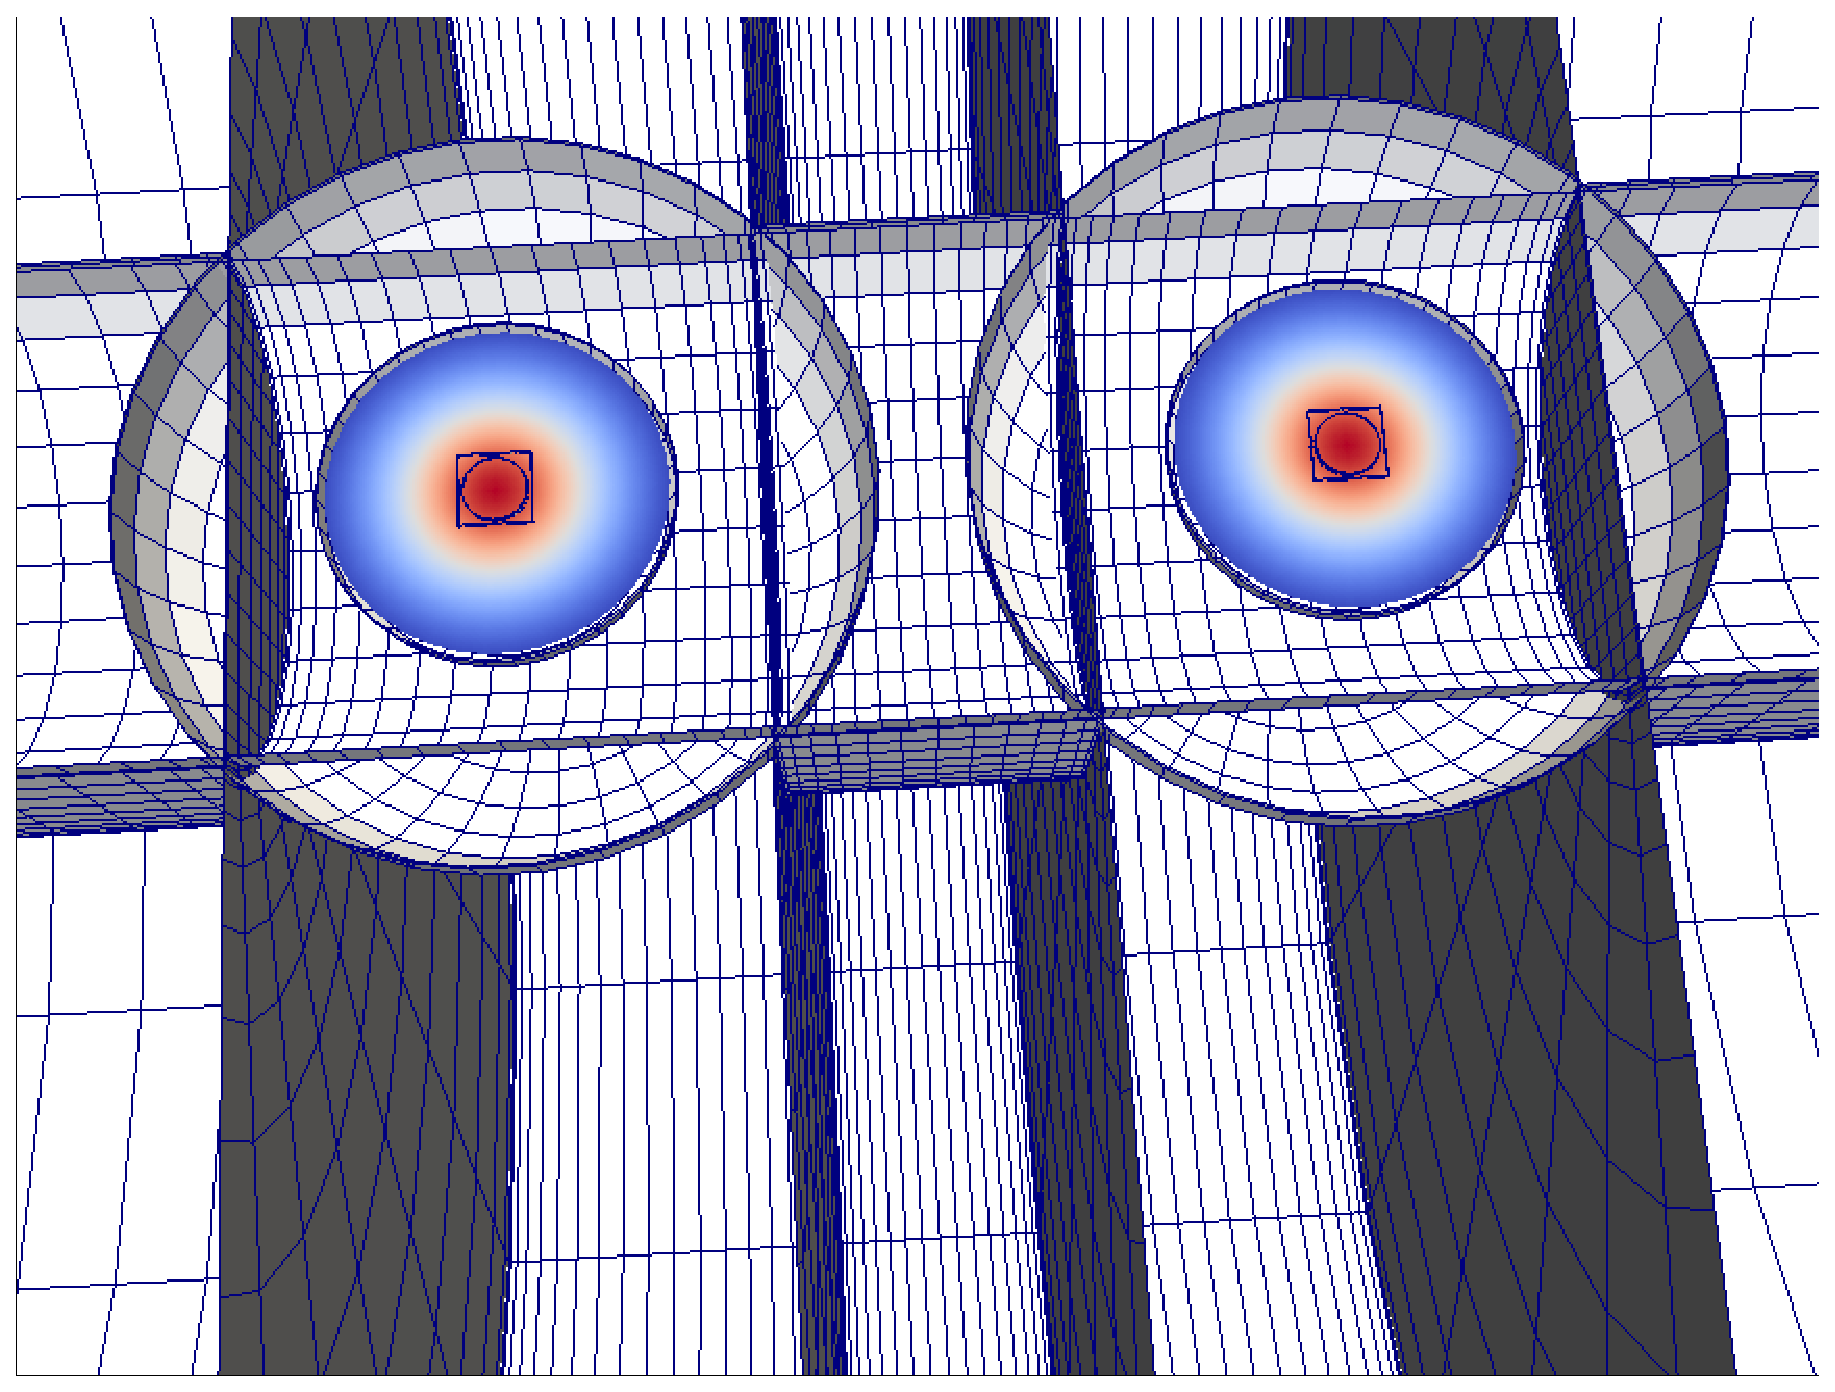
\includegraphics[width=0.95\columnwidth,trim=0 185 0 0, clip=true]{TheDomain}
\caption{\label{fig:TheDomain} A visualization in the x-y plane of the
  domain decomposition used in our initial data solve. The colour map
  represents the density of the stars.  }
\end{figure}

In the previous sections, we have reduced the Einstein
  constraints, Eqs.~(\ref{eq:XCTS-Shift})--(\ref{eq:XCTS-Lapse}), as
  well as the continuity equation~(\ref{eq:Continuity}) to elliptic
  equations.  We solve these equations with the multi-domain
  pseudo-spectral elliptic solver developed in~\cite{Pfeiffer2003}, as
  modified in~\cite{FoucartEtAl:2008} for matter.  The
  computational domain is subdivided into individual subdomains as
  indicated in Fig.~\ref{fig:TheDomain}: The region near the center of
  each star is covered by a cube, overlapping the cube is a spherical
  shell which covers the outer layers of the star.  The outer boundary
  of this shell is deformed to conform to the surface of the star.
  This places the discontinuous transition from matter to vaccum at a
  subdomain-boundary, and preserves exponential convergence of the
  spectral method.  Another spherical shell surrounds each star.  The
  inner shells representing the stars and their vicinity are embedded
  into a structure of five concentric cylinders with three rectangular
  blocks along the axis connecting the centers of the neutron stars,
  which overlap the inner spherical shells.  The clyinders/blocks, in
  turn are overlapped at large radius by one further spherical shell
  centered half-way between the two neutron stars.  Using an inverse radial mapping, the outer radius of the outer sphere is placed at $10^{10}$, representing infinity.

  All variables are decomposed into terms of
appropriate basis functions, depending on the subdomain. The
resolution (i.e., the number of colocation points used) of each domain
is chosen at the start of the initial data solve, and then
subsequently modified several times using the adaptive procedure
described below. In this paper to discuss the total resolution of the
domain, we use the notation 
\begin{equation}
N^{1/3} = \left(\sum
N_i\right)^{1/3},
\end{equation}i.e., the cube root of the total number of
collaction points in all subdomains.  

%%%%%%%%%%%%%%%%%%%%%%%%%%%%%%%%%%%%%%%%%%%%%%%%%%%%%%%%%%%%%%%%
\subsection{Explanation of Numerical Solver}
\label{sec:IDalgorithm}
%%%%%%%%%%%%%%%%%%%%%%%%%%%%%%%%%%%%%%%%%%%%%%%%%%%%%%%%%%%%%%%%

Construction of initial data for rotating binary neutron stars
begins with selecting the physical properties of the system: the equation of
state of nuclear matter, the coordinate separation $d$ between the
neutron stars, the masses $M_1$ and $M_2$ of the two stars, and their
spin vectors ${\bm \omega}_{\rm rot,1}$ and ${\bm \omega}_{\rm
  rot,2}$. We also choose the orbital angular frequency $\Omega_0$
and the initial inspiral rate $\dot{a}_0$.  
Values for $\Omega_0$ and $\dot{a}_0$ can be determined either by matching the values found for a quasi-equilibrium irrotational binary with the same
physical parameters or by following the eccentricity reduction method
developed by Pfeiffer et al.~\cite{Pfeiffer-Brown-etal:2007}. Finally, we use a flat conformal metric, $\tilde\gamma_{ij}=\delta_{ij}$,
and maximal slicing, $K=0$.
%\harald{We also choose a conformal metric $\tilde\gamma_{ij}$ and the trace of the extrinsic curvature $K$ by \red{[Fill in]}.}

Once all these quantities are fixed, we need to solve self-consistently Eqs.~(\ref{eq:XCTS-Shift})--(\ref{eq:XCTS-Lapse}) for the Einstein-constraints, the continuity equation Eq.~(\ref{eq:Continuity}), while simultaneously satisfying conditions to enforce the desired masses of the stars. 
To do so, we follow an iterative procedure developed originally for black hole-neutron star
binaries~\cite{FoucartEtAl:2011}.

First, we initialize initial guesses
for the conformal metric and hydrodynamical variables 
%\red{[State precisely which hydrodynamic variables are being initialized]}
, using an
analytical superposition of two isolated boosted neutron stars.

We then obtain constraint-satisfying initial conditions by applying
the following iterative procedure, where $n$ represents the iteration number:
\begin{enumerate}
\item \label{step:1} 
  Solve the XCTS system for $X=(\beta^i,\Psi,\alpha \Psi)$,
  assuming fixed values of the conformal source terms
  $(\tilde{E},\tilde{S},\tilde{J}^i$). The new value $X^{n+1}$ of the
  metric variables is obtained from their old value $X^n$ and,
  following the relaxation scheme used in \cite{FoucartEtAl:2008} the
  solution of the XCTS equations $X^*$ using
\begin{equation}
\label{eq:Relaxation}
X^{n+1}=0.3X^*+0.7X^n.
\end{equation}
%\red{[motivate/give reason for this linear combination.  Could be as simple as ``we follow Foucart et al, and set...'']}
% \item If the spin vectors are parallel to the orbital angular
%   momentum, enforce equatorial symmetry on $X$.
% \red{[Specify how.  Perhaps  ``by averaging $X(x,y,z)$ and
%   $X(x,y,-z)$'' or ``by replacing the data for $z<0$ by the data for
%   $z>0$''?]}
% \nick{Although it would have been sensible, I did not actually
%   specifically enforce Z symmetry in the initial data in these cases,
%   so I am just going to take this out I think}
\item Locate the surface of each star.  Representing the surface in polar coordinates centered on each star as $R_s^n(\theta,\phi)$, we determine $R_s^n$ to satisfy~\cite{FoucartEtAl:2008} $h(R^n_{\rm
  s}(\theta,\phi),\theta,\phi)=1$.
To ensures that the grid-boundary $R_b$ converges to the surface of the star, we occassionally modify the numerical grid such that $R_b(\theta,\phi)=R^n_s(\theta,\phi)$.  Because this requires a re-initialization of the elliptic solver, the grid is only modified the stellar surface has settled down, specifically, if
\begin{equation}
||R^n_{\rm s} - R^{n-1}_{\rm s}||_2 < 0.1*||R^n_{\rm s} - R_b||_2.
\end{equation}
Here $||\;.\;||_2$ denotes the L2-norm over the surface.
%\item Measure the ADM linear momentum $P^{i,n}_{\rm ADM}$. If for
%  the largest component of $P^{i}_{\rm ADM}$ we have
%  $|P^{i,n}_{\rm ADM}-P^{i,n-1}_{\rm ADM}|<0.1|P^{i,n}_{\rm ADM}|$, we
%  move the center of one of the neutron star to drive ${P}^i_{\rm
%    ADM}$ to $0$. The procedure to choose the new location of the
%  neutron star center is described in more details in Henrikson et
%  al.~\cite{Henriksson:2014tba}. We do not
%  control the z-component of ${P}^i_{\rm ADM}$.  For aligned spin systems, symmetry requires $P^z_{\rm ADM}=0$.  For precessing systems, this symmetry is no longer present, and for S.4x, we find $P^z_{\rm ADM}\sim 8.7\times 10^{-7}$.  This value is quite small and we neglect its impact in the present study.

\item For each neutron star, fix the constant in Euler's first
  integral so that the baryon mass of the neutron star matches the desired
  value.  We compute the baryon mass as a function of the Euler constant $C$
through %\roland{$C$ has not been defined yet}
\begin{equation}
M^b_{\rm NS} = \int_{\rm
  NS}\rho_0\Psi^6\sqrt{\frac{1}{1-\gamma_{ij}U^iU^j}}dV,
\end{equation}
%\red{Harald suspects $\phi$ is the conformal factor.  In contrast to Foucart, we use $\Psi$ for conformal factor, and $\phi$ for the velocity potential. Check and correct.}  
%\red{Check entire paper for $\psi\leftrightarrow\phi$ typos. }
and utilize the secant method
to drive the mass to the desired value.
\item If desired, adjust the orbital frequency to ensure force-balance at the
  center of each star by solving Eq.~(\ref{eq:OmegaEq}). This step is
  skipped if the orbital frequency is fixed through iterative eccentricity removal, cf. Sec.~\ref{sec:EccRemoval}.
\item Solve the elliptic equation for the velocity potential $\phi$,
  and obtain the next guess for $\phi$ using the same relaxation
  method shown in Eq.~\ref{eq:Relaxation}.
\item  Check whether all equations are satisfied to the desired accuracy. If yes, proceed.  If no, return to Step~\ref{step:1}.
\item Compute the truncation error of the current solution by
    examining the spectral expansion of the XCTS variables.  If this
    truncation error is undesirably large (typically, if it is
    $>10^{-9}$), then adjust the number of grid-points in the
    domain-decomposition and return to Step~\ref{step:1}.  The adjustment
is based on the desired target truncation eror and the measured convergence rate of the solution, cf.~\cite{Szilagyi:2014fna}.
%\red{[Sergei changed his AMR algorithm jsut a few weeks ago, so almost certainly you are doing this differently.  Saver to cite Szilagyi]}
\end{enumerate}
%\sout{Once this is done, we evaluate the accuracy of the current solution by
%measuring the truncation error of the spectral expansion of the XCTS
%variables. If that truncation error has not reached the desired target
%(usually $10^{-9}$), we increase the resolution in each subdomain. The
%method used to select the next resolution, which uses the observed
%convergence of the spectral expansion of the XCTS variables to guess
%the change of resolution required to obtain a desired improvement in
%accuracy, is described in more details in Ossokine et al. (in prep).
%We then go back to the above iterative procedure to obtain a
%constraint-satisfying solution on the new grid.}

\subsection{Quasi-Local Angular Momentum}
\label{sec:QLSpinExplanation}

The goal of the present paper is to construct spinning NS-NS initial data and to evolve it.  Therefore, we need diagnostics to measure the NS spin, for which we use techniques originally developed for black holes.
It is common to discuss the spins of black holes in terms of their
dimensionless spin $\chi$,
\begin{equation}\label{eq:chi}
\chi = \frac{S}{M^2}.
\end{equation}
Here, $S$ is the angular momentum of the black hole, and $M$ is its
Christodoulou formula~\cite{Christodoulou70},
\begin{equation}\label{eq:ChristodoulouMass}
M^2 = M_{\rm irr}^2 + \frac{S^2}{4M_{\rm irr}^2}.
\end{equation}
The irreducible mass $M_{\rm irr}$ is defined based on the area of the
hole's apparent horizon, $M_{\rm irr}=\sqrt{A/16\pi}$. The angular
momentum is computed with a surface integral over the apparent
horizon~\cite{BrownYork1993,Ashtekar2001,Ashtekar2003},
\begin{equation}\label{eq:QLspin}
S= \frac{1}{8\pi}\oint_{\mathcal{H}}\phi^is^jK_{ij}dA
\end{equation}
where $\mathcal{H}$ is the black hole's apparent horizon, $s^j$ is the
outward-pointing unit-normal to $\mathcal{H}$ within the $t=$const
hypersurface, and $\phi^i$ is an azimuthal vector field tangent to
$\mathcal{H}$.  For spacetimes with axisymmetry, $\phi^i$ should be
chosen as the rotational Killing vector.  In spacetimes without an
exact rotational symmetry (e.g. the spacetime of a binary black hole
system), one substitutes an \emph{approximate Killing
  vector}\cite{Cook2007,Lovelace2008} (AKV).  Ref.~\cite{Lovelace2008}
introduces a minimization principle to define $\phi^i$, resulting in
an Eigenvalue problem. The three eigenvectors with the lowest
eigenvalues (i.e. smallest shear) are taken and used to compute
the three components of the spin.

In this paper, we explore the application of quasi-local spin measures
to neutron stars.  In the absence of apparent horizons $\mathcal{H}$,
we need to choose different surface(s) to evaluate Eq.~(\ref{eq:QLspin}). 

When constructing initial data, the stellar surface ${\cal S}$ is
already determined, so one obvious choice is to integrate over the
stellar surface ${\cal S}$.  To estimate the ambiguity in quasi-local
spin, we furthermore compute $S$ by integrating over coordinate
spheres with radii ranging from just outside ${\cal S}$ to larger by
about $70\%$.  During the evolution, the stars change shape and
may even loose mass in tidal tails.  Because of these complications,
the SpEC evolution code does not track the location of the
stellar surface during the evolution, and we shall only
monitor $S$ on coordinate spheres.

It is useful to compute a dimensionless spin $\chi$, for instance, for
post-Newtonian comparisons.  In the absence of a horizon,
Eq.~(\ref{eq:ChristodoulouMass}) is meaningless and we need a different
choice for the mass-normalization.  Instead, we normalize by each 
star's ADM mass, $M_{\rm{ADM, star}}$, i.e. 
\begin{equation}
\chi\equiv \frac{S}{M_{\rm ADM, star}^2}.
\end{equation}
The ADM mass is determined by computing the ADM mass of an equilibrium configuration of a single uniformly rotating polytrope with the same baryon mass and angular momentum as those measured in our binary systems.


%This mass is determined by solving
%\begin{equation}\label{eq:M_ADM-def}
%E_{\rm ADM} = 2M_{\rm ADM, star} - M_{B}\Omega_0^2D^2,
%\end{equation}
%where we used the virial theorem and assumed equal masses.  Equation~(\ref{eq:M_ADM-def}) could
%be improved with a post-Newtonian formula, which might modify
%$M_{\rm ADM, star}$ by a fraction of a percent.  However, since we use
%$M_{\rm ADM, star}$ only to normalize $\chi$, such small corrections
%are beyond the scope of the present work.
The results of the
quasi-local spin measures are described in
section~\ref{sec:QLSpinProperties}, which shows that this procedure is
numerically robust.
%\roland{this is an unusual
%(to me)
%definition of the ADM mass of the individual stars. I would have expected this
%to be the ADM mass of ``a similar object but with no companion''. Here however
%you define the ADM mass to be half of the ADM energy (=mass) of the system
%after you subtracted some guess for the orbital kinetic energy.}


Finally, let us discuss, from an order of magnitude perspective, how
the star's dimensionless spin is related to its physical quantities.
We start with the Newtonian relation $S=2\pi I/P$ between angular
momentum $S$, moment of inertia $I$, and rotational period $P$.
Writing further $I=f\,R^2\,M$, with the dimensionless constant $f$
depending on the stellar density profile, we have 
\begin{align}
\chi&\sim\frac{2\pi c}{G}\frac{fR^2}{PM} \nonumber\\
&=
0.48\,\Big(\frac{f}{0.33}\Big)\Big(\frac{R}{12{\rm
    km}}\Big)^{\!2}\Big(\frac{M}{1.4M_{\odot}}\Big)^{\!-1}\Big(\frac{P}{1{\rm
    ms}}\Big)^{\!-1}\!\!.
\end{align}
The factor $c/G$ arises from the transition to geometric units. 

This --quite simplistic-- estimate shows that millisecond pulsars will
have appreciable dimensionless spin $\chi$.  Centrifugal breakup of
rapidly rotating neutron stars happens at a dimensionless spin in the
range $0.65-0.70$~\cite{Lo:2010bj}, with only small dependence on the
equation of state and neutron star mass.  Ansorg et
al~\cite{Ansorg:2003br} studied in detail $\Gamma = 2$ polytropes, the
equation of state we use here.  Ref.~\cite{Ansorg:2003br} finds the
dimensionless spin at mass-shedding of $\chi=0.57$.

\section{Initial Data Results}
\label{sec:ID}

%\subsection{Code Tests}

In this section, we will demonstrate that our code can robustly
construct contraint-satisfying initial data for BNS systems with
arbitrary spins. As discussed in section~\ref{sec:IDalgorithm}, our code consists of a
linear solver that runs for a number of iterations at constant
resolution, and then the resolution is increased and this process
restarts. We will therefore demonstrate that appropriate quantities
converge with both the iterations of the linear solver, and with
resolution as the resolution increases. 



%\begin{table*}
%\begin{tabular}{l|cc|ccc|cc}
%Name & $M^b_{\rm NS}$ & ${\bm \omega}$ & $D_0$ & $\Omega_0 \times 10^{3}$ & $\dot{a}_0 
%\times 10^{5}$  & $M_{\rm ADM}$ &  $\vec\chi$ 
%\\\hline
%S0.4z & 1.7745 & $0.01525\hat{z}$ & 47.2 & 5.09594 & -1.75 & 1.68711 & $0.35923\hat{z}$ \\
%S-0.05z & 1.7745 & $-0.00273\hat{z}$ & 47.2 & 5.11769 & -1.71 & 1.67912 & $-0.047866\hat{z}$ \\
%S0.4x & 1.7745 & $0.01525\hat{x}$ & 47.2 & 5.10064 & -2.36 & 1.68761 & $0.35418\hat{x}$\\
%\end{tabular}
\begin{table*}
\begin{tabular}{l|cc|ccc|cc}
Name & $M^b_{\rm NS}$ & ${\bm \omega}$ & $D_0$ & $\Omega_0 \times 10^{3}$ & $\dot{a}_0 
\times 10^{5}$  & $M_{\rm ADM}$ &  $\vec\chi$ 
\\\hline
S.4z & 1.7745 & $0.01525\hat{z}$ & 47.2 & 5.09594 & -1.75 & 1.648 & $0.3765\hat{z}$ \\
S-.05z & 1.7745 & $-0.00273\hat{z}$ & 47.2 & 5.11769 & -1.71 & 1.640 & $-0.05018\hat{z}$ \\
S.4x & 1.7745 & $0.01525\hat{x}$ & 47.2 & 5.10064 & -2.36 & 1.648 & $0.3714\hat{x}$\\
\end{tabular}
\caption{\label{tab:InitialData}
%\red{[Two masses should be given:  Toward the left of the table, the mass you fixed when constructing the ID ($M_{\rm ADM}$?), toward the right, the other mass that is read off after construction of the ID ($M_b$?)]}
Parameters for the initial data sets used in testing the initial data solver: $M^b_{\rm NS}$ and $\omega^i$ are baryon mass and rotational parameter for either neutron star (the same values are used); $D_0$, $\Omega_0$ and $\dot a_{0}$ represent coordinate separation between the centers of the stars, the orbital frequency, and the radial expansion; $\vec\chi$ is the dimensionless spin magnitude computed from the initial data set. In each case we use a polytropic equation of state, $P=\kappa\rho_0^{\Gamma}$, with $\Gamma=2$ and $\kappa=123.6$.}
\end{table*}


\subsection{Convergence of the Iterative Procedure}

At each step of the iterative procedure, the Euler constant of each
star is modified to achieve a desired stellar baryon mass, based on
the current matter distribution inside the star.  We expect that the Euler constant converges during the iterations at a fixed resolution. Figure~\ref{fig:EulerConstConvergence}  shows the behavior of the Euler Constant during iterations at the lowest initial data resolution, R0.  
We show three runs of interest, one
with large aligned spins ({\tt S.4z}), one with large precessing spin ({\tt S.4x}), and one with small anti-aligned spins ({\tt S-.05z}). 
% \red{[If we point to the jumps, then it would be good to have a reason for them.  They are equally spaced, every 10 iterations, so there probably {\em is} a certain adjustment in the code that causes them (e.g. re-initialization of the stellar surface?). But let's try to live simply.]} 
In all three cases we see agreement between neighboring iterations at the
$10^{-5}-10^{-6}$ level by the end of iterating at this resolution. At the highest resolutions, these
differences are down to, typically, the $10^{-9}-10^{-10}$ level.

%%%%%%%%%%%%%%%%%%%%%%%%%%%%%%%%%%%%%%%%%%%%%%%%%%%%%%%%%%%%%%%%
\begin{figure}
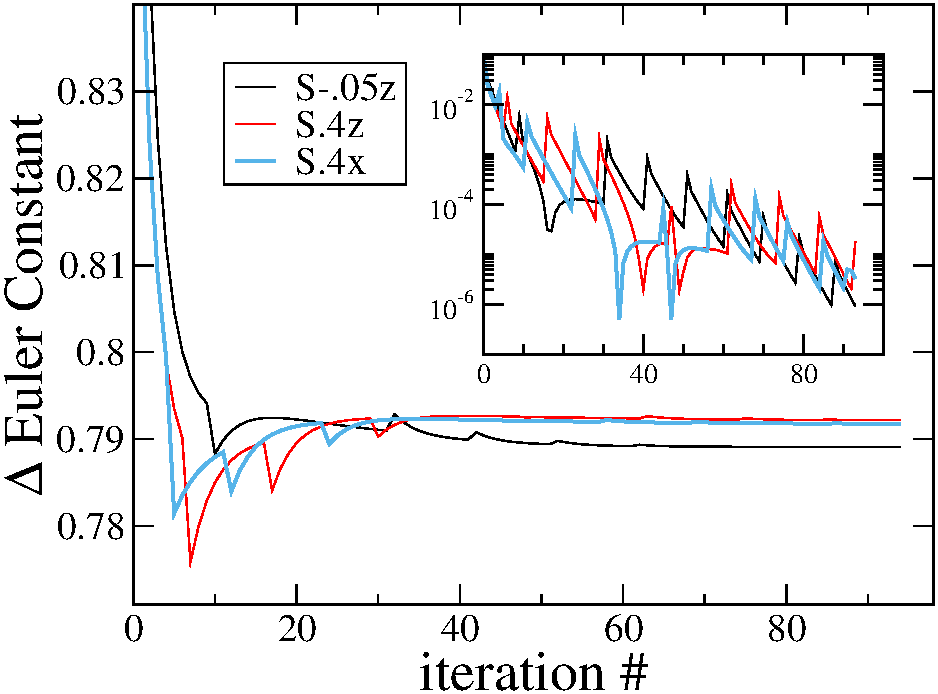
\includegraphics[width=0.95\columnwidth]{EulerConstConvergence}
\caption{\label{fig:EulerConstConvergence}
%\red{[Adjust font sizes and tick-sizes, such that the inset has smaller fonts and ticks.  Start inset y-axis at $10^{-1}$, to eliminate one of the labels on the y-axis.  Increase legend font-size to $\ge$ the font-size on axes]}
Convergence of the Euler
  constant during iteration at the lowest resolution R0. The inset shows the difference
  between values at subsequent iterations.}
\end{figure}
%%%%%%%%%%%%%%%%%%%%%%%%%%%%%%%%%%%%%%%%%%%%%%%%%%%%%%%%%%%%%%%%

%As described in section~\ref{sec:IDalgorithm}, the code occasionally
%adjusts the centre of a star in order to zero out the ADM linear
%momentum, $P$ of the system. The ADM linear momentum is
% given by~\cite{ADM,York:1979} an integral
%  over a surface $\mathcal{S}_\infty$ at space-like infinity.  To
%reduce sensitivity to numerical errors, we follow
%Foucart~\cite{FoucartEtAl:2008} and use Gauss' law to rewrite it as a
%surface integral over a surface $\mathcal{S}$ at finite radius.  The
%resulting volume term vanishes for conformal flatness and maximal
%slicing, and one finds
%\begin{equation}
%P^{i}_{\rm ADM} = \frac{1}{8\pi}\oint_{S_{\infty}}K^{ij}dS_j
%=\frac{1}{8\pi}\oint_{\mathcal{S}} \psi^{10}K^{ij}dS_j.
%\end{equation}
%In
%figure~\ref{fig:PADMConvergence} we plot both $|P_x|$ and $|P_y|$ as
%the lowest resolution iterates, for our three cases of interest, demonstrating %the convergence
%we expect. They then level off at a value typically $10^{-5} -
%10^{-6}$, at which point this process is probably limited by
%resolution. Larger spins ({\tt S0.4z} and {\tt S0.4x}) result in somewhat larger residuals than the
%low spinning case. At the highest resolution, the solver achieves $P_{\rm ADM}\lesssim 10^{-8}$.  \red{[It's odd that you show of the worst case (i.e. R0).  Can you plot Padm at high resolution, or at {\em all} resolutions?]} \nick{Let's go over these plots together, some strange features I didn't notice before.}

%\begin{figure}
%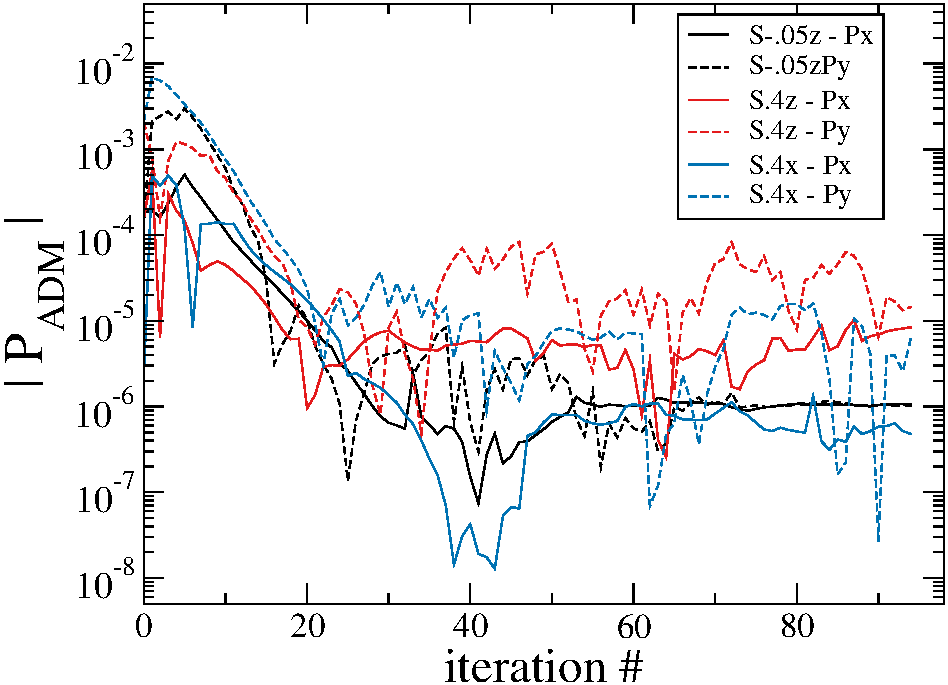
\includegraphics[width=0.95\columnwidth]{PADMConvergence}
%\caption{{\label{fig:PADMConvergence}} Convergence of the absolute
%  values of the x and y components of the ADM linear momentum. This is
%  shown as the lowest resolution iterates for our three cases of
%  interest. Our code tries to re-centre the stars so as to drive this
%  quantity to zero.}
%\end{figure}

%\begin{itemize}
%\item \green{To include: Convergence of $X_{NS}$?}
%\item \green{To include: Convergence of $M_{NS}$?}
%\end{itemize}

\subsection{Convergence of the Solution}

Having established that our iterative procedure converges as intended,
we now turn out attention to the convergence of the solution with
resolution. To demonstrate it, we will look at the Hamiltonian and
momentum constraints, and the differences between measured physical
quantities - the ADM energy and ADM angular momentum, and the surface
fitting coefficients of the stars. As our initial data representation
is fully spectral, we expect that these quantities should converge
exponentially with resolution. Note that when we discuss the value of
a quantity at a certain resolution, we are referring to the value of
that quantity after the final iterative step at that
resolution.  
%\harald{ \red{[Harald thinks the following sentences do no longer apply. Correct?]}\sout{
%\red{[Move next sentence to the first figure that shows this effect.]}
%Finally, the reader will notice
%\roland{as a reader I am not sure what I notice, nor do I see which figure I should notice it in} 
%that one initial data set
%(S.4z) has one more data point that the others. This is because it
%just happened to take one more iteration to reach the termination
%criterion than the other initial data sets did.
%\roland{this is lots of internal details of the solver and code}


Figure~\ref{fig:HamMom} shows the convergence of the Hamiltonian
constraint and the Momentum constraint for our three runs of
interest.  These are computed during the last iterative solve at each
resolution.  The data plotted are computed as
\begin{equation}
H = ||\frac{R_\Psi}{8\Psi^5}||,
\end{equation}
\begin{equation}
M = ||\frac{R_{\beta}}{2\alpha\Psi^4}||.
\end{equation}
Here $R_\Psi$ and $R_\beta$ denote the residuals of Eqs.~(\ref{eq:XCTS-ConformalFactor}) and~(\ref{eq:XCTS-Shift}), respectively
, and $||\,.\,||$ represents the \harald{root-mean-square value over grid-points of} the
 entire computational grid. 
This plot demonstrates that our initial
data solver converges  exponentially with resolution, even for
very high spins, which gives confidence that we are indeed correctly
solving the Einstein Field Equations.

\begin{figure}
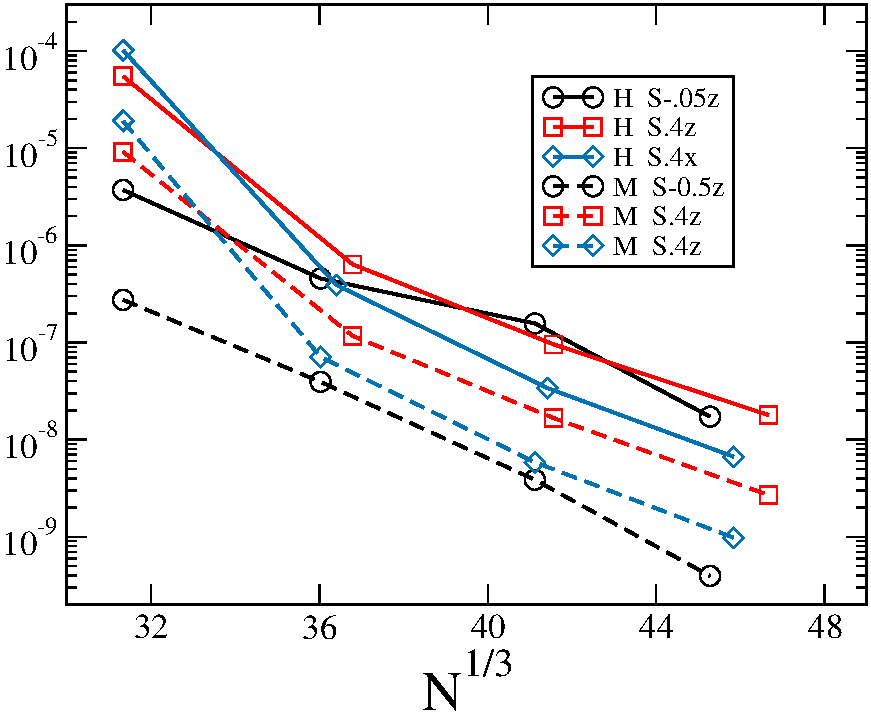
\includegraphics[width=0.95\columnwidth]{HamMom}
\caption{{\label{fig:HamMom}}Hamiltonian and Momentum constraints as a function of resolution $N$. We see exponential
  convergence in all cases.}
\end{figure}

 The surface of the star is represented by a spherical harmonic expansion:
\begin{equation}
R_s(\theta,\phi) = \sum^{l_{\rm max},m_{\rm
    max}}_{l,m}c_{lm}Y_{lm}(\theta,\phi),
\end{equation}
where $l_{\rm max}= m_{\rm max} = 11$, unless stated otherwise.
The stellar surface is located by finding a constant enthalpy surface, cf. Sec.~\ref{sec:IDalgorithm}, and the spherical subdomains that cover the start are deformed to conform to $R_s(\theta,\phi)$.
To establish convergence of the position of the stellar surface we
introduce the quantity
\begin{equation}
\label{eq:Deltac}
\Delta c(i) = \frac{1}{l(l+1)} \sqrt{\sum^{l_{\rm max},m_{\rm
      max}}_{l,m}\left(c_{lm}(i)-c_{lm}(N)\right)^2}.
\end{equation}
Here $i$ refers to the $i^{\rm th}$ resolution in the initial data,
and $N$ refers to the final resolution. Figure~\ref{fig:ClmDif} plots $\Delta c(i)$ vs. resolution.  The surface location converges exponentially to better than $10^{-8}$.

\begin{figure}
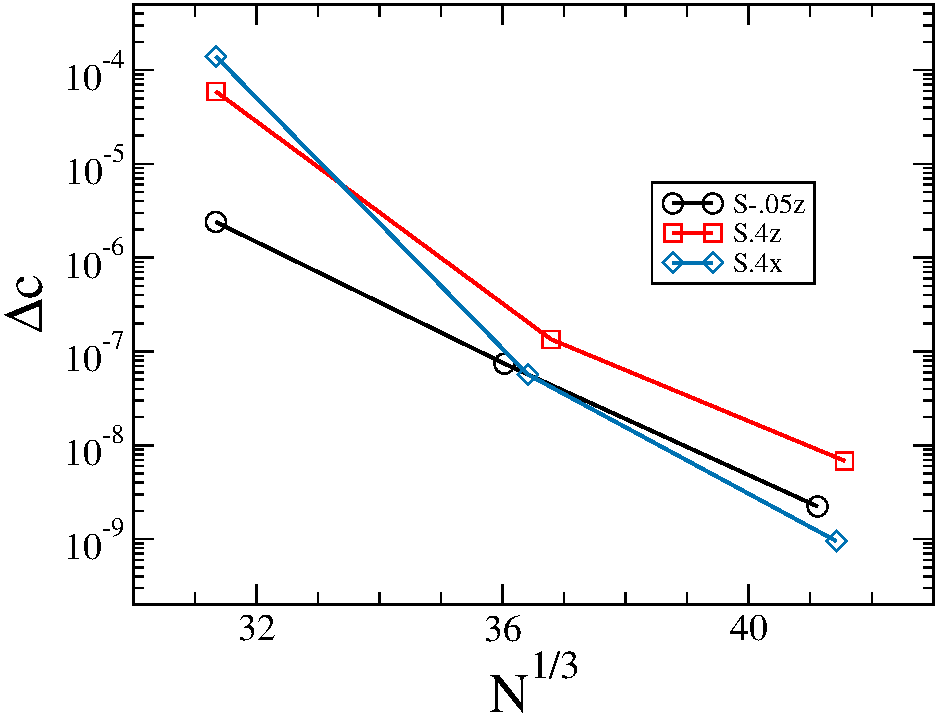
\includegraphics[width=0.95\columnwidth]{ClmDif}
\caption{{\label{fig:ClmDif} Convergence of the location of the stellar surface}.
  Plotted is $\Delta c$ as defined in Eq.(~\ref{eq:Deltac}), for three representative configurations.}
\end{figure}

Finally, we assess the overall convergence of the solution through
the global quantities $E_{\rm ADM}$ and $\left|J^i_{\rm ADM}\right|$.  \harald{
%\sout{These are evaluated as
%integrals over the outer boundary of the domain, $S_{\infty}$:}
%Similar to $P^i_{\rm ADM}$, 
The surface integrals at infinity in these two quantities are recast using Gauss' law (cf.~\cite{FoucartEtAl:2008}):
% \red{[Here and everywhere else: correct $P_{\rm ADM}$ and $J_{\rm
 %    ADM}$ to display them consistently as vectors (i.e. either
  % boldface, or with an index.]}
}
\begin{align}
E_{\rm ADM} &= -\frac{1}{2\pi}\oint_{S_{\infty}}\delta^{ij}\partial_i\Psi\, dS^j\nonumber \\
&= -\frac{1}{2\pi}\oint_{S}\delta^{ij}\partial_i\Psi\, dS_j  +\frac{1}{2\pi}\int_{\mathcal{V}}\delta^{ij}\partial_i\partial_j\Psi\,dV,
\end{align}
and
% \begin{align}
% J^{i}_{\rm ADM} 
% & = \frac{1}{8\pi}\oint_{S_{\infty}}\epsilon^i{}_{jk}x^jK^{kl}dS_l\nonumber\\
% & = \frac{1}{8\pi}\oint_{S}\epsilon^i{}_{jk}x^jK^{kl}dS_l.
% \end{align}
\begin{align}
J^{z}_{\rm ADM} 
& = \frac{1}{8\pi}\oint_{S_{\infty}}\left(xK^{yj}-y K^{xj}\right)dS_j\nonumber\\
& = \frac{1}{8\pi}\oint_{S}\left(xK_{yi}-yK_{xi}\right)\delta^{ij}\Psi^2\,dS_j.
\end{align}
\harald{Here $\mathcal V$ is the volume outside $S$, and the integrals are evaluated in the flat conformal space.  To obtain the other components of $J_{\rm ADM}^i$, cyclically permute the indices x,y,z.}
 We define the quantities $\Delta E$ and $\Delta J$ as the absolute fractional difference in these quantities between the current resolution and the next highest resolution. These are plotted in figure~\ref{fig:EADMConvergence}.  In all cases we find clear
exponential convergence. In general, we find
agreement at the $10^{-7}-10^{-8}$ level by the final
resolution.
%For the S-.05z and S.4x cases we find what looks like exponential
%convergence. However, for the S.4z case we find that the difference
%becomes limited at the $10^{-6}$ level. This could come from the fact
%that we do not specifically control the angular momentum of the stars
%and so any residual uncertainty in the angular momentum could be
%translated into uncertainty in the ADM angular momentum - this will
%be further discussed in section XX.\red{Look into this more!}

\begin{figure}
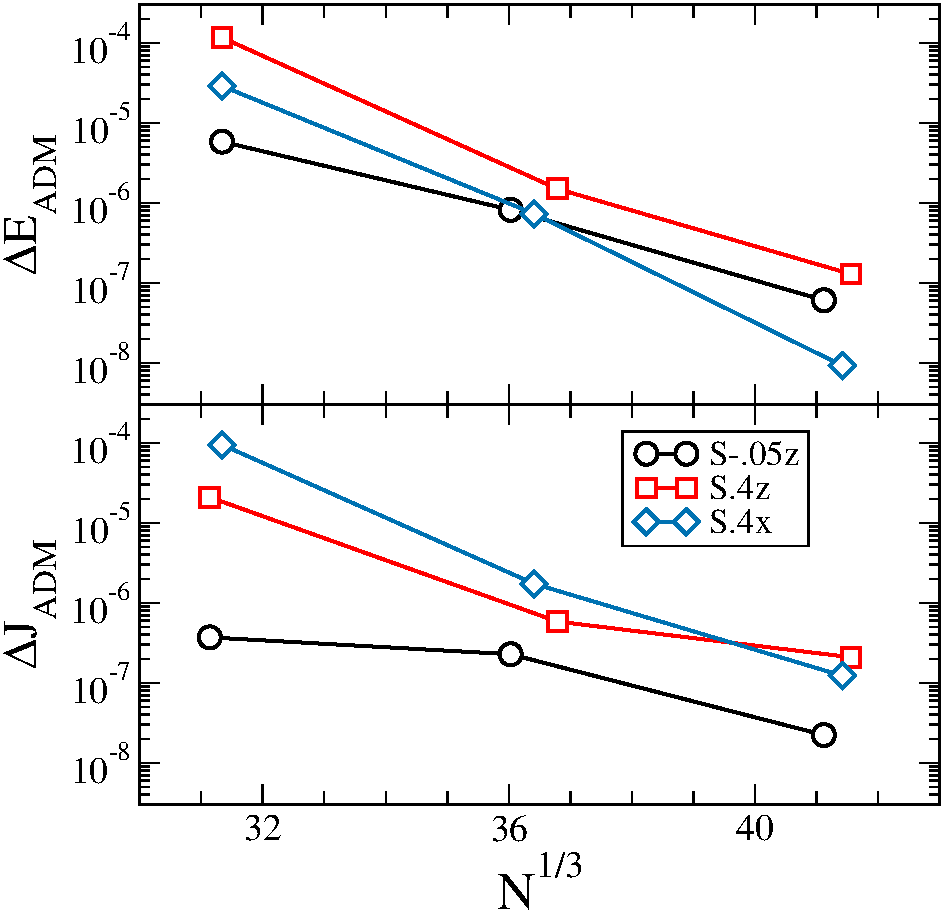
\includegraphics[width=0.95\columnwidth]{EADMConvergence}
\caption{{\label{fig:EADMConvergence}} Convergence of ADM-energy and the magnitude of the ADM-angular momentum.  Shown are the fractional differences between neighboring resolutions, as a function of the lower resolution.
 %\red{[Roland:  Can you explain why S-0.05z crosses the other lines?]} \roland{I cannot give an ad-hock explanation. I am not sure if I would be very concerend about the crossing itself. These are after all different physical systems. All that the crossing means is that the S-0.05z run converges more slowly than the other ones. In order to make me concerned one would have to have a series of runs SZZz where ZZ would go from -0.05 to say 0.05 then to 0.4 to check if there is some monotonic behaviour with resolution of the converegence speed.}}
}
\end{figure}

% \begin{figure}
% 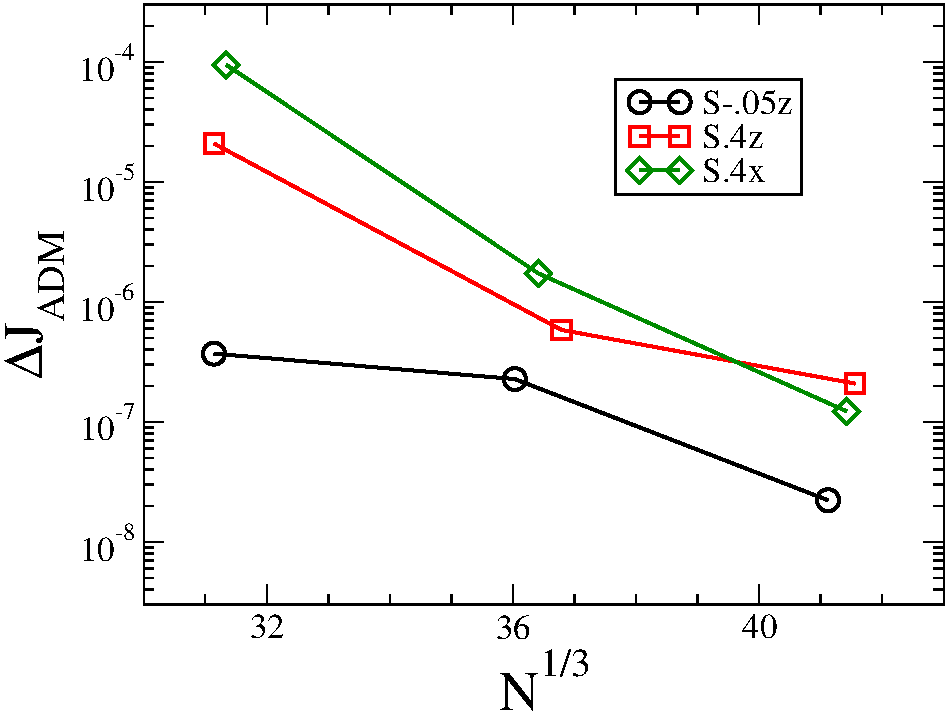
\includegraphics[width=0.95\columnwidth]{JADMConvergence}
% \caption{{\label{fig:JADMConvergence}} Convergence of the absolute
%   fractional difference of the ADM Angular Momentum with the final
%   resolution. This is plotted for our three runs of interest. In all
%   the cases we see nearly exponential convergence. }
% \end{figure}






%\subsection{Convergence Tests} \label{sec:ConvergenceTests} In this
%section we will present tests of our code to show that it
%converges. Convergence in this sense can mean one of two
%things. First, that during the iterative procedure done at fixed
%resolution, quantities which are changed at each iteration converge
%to some fixed value as the iterations go on. Second, that as the
%resolution of domain is increased, quantities like the constraints
%tend to vanish, and physical quantities converge to some fixed
%value. All the results presented in these sections will focus on our
%three runs of interest.

%\subsubsection{Convergence of the Linear Solver}


%\begin{itemize} \item In figure 1 we plot the Euler constant as Lev0
%\red{Need to define what Lev means, or create a better nomenclature}
%iterates. This is shown for al three of our runs of interest. This
%plot shows that in our initial data, successive iterative solves at
%the same resolution lead physical quantities like the Euler constant
%to settle down to a constant vaue before the resolution is eventually
%incrased.  \item In figures 2 and 3 we plot the convergence of the
%Hamiltonian constraint and Momentum constraints respectively for our
%three runs of interest. These are computed during the last iterative
%solve at each resolution. The Hamiltonian constraint is calculated
%as \begin{equation} H = ||\frac{\delta\Psi}{8\Psi^5}|| \end{equation}
%and the Momentum constraint is calculated as \begin{equation} J =
%||\frac{\delta{\beta}}{2\alpha\Psi^4}|| \end{equation} \red{Need a
%better symbol than J? What is typical in the literature?}. Here
%$\delta\Psi$ is the residual conformal factor, $\delta\beta$ is the
%residual shift \red{How are these computed?  Unclear to me}, and $||$
%represents the L2 norm evaluated over the whole computational
%grid. These two plots demonstrate that our initial data solver
%converges (nearly exponentially) with resolution, even for very high
%spins, which gives confidence that we are correctly solving the
%Einstein Field Equations.

%\item As we'll later discuss, we measure the spin of the star on a
%surface $S(\theta,\phi)$. The surface is found by looking for a
%constant enthalpy $h=1$ surface. It is expressed as a sum of
%spherical harmonics \begin{equation} S(\theta,\phi) = \sum^{l_{\rm
%max},m_{\rm max}}_{l,m}c_{lm}Y_{lm}(\theta,\phi) \end{equation} where
%$l_{\rm max} = m_{\rm max} = 11$ unless otherwise stated. To believe
%that the spin measured on this surface is sensible, it is necessary
%to believe that the surface itself is sensible. Therefore this
%surface finder should converge in some meaningful sense. To quantify
%this, we introduce the quantity \begin{equation} \delta c(i) =
%\frac{1}{l(l+1)} \sqrt{\sum^{l_{\rm max},m_{\rm
%max}}_{l,m}\left(c_{lm}(i)-c_{lm}(N)\right)^2} \end{equation} Here
%$i$ refers to the $i^{\rm th}$ resolution in the initial data, and
%$N$ refers to the final resolution. In figure~\ref{fig:ClmDif} we
%plot this quantity for our three cases of interest. Convergence is
%clearly demonstrated.




%\item \green{To include: Convergence plots of Px and Py similar to
%Euler constant?}  \item \green{To include: Convergence plots of
%Surface fitting coeffs?}  \item \green{To include: Convergence plots
%of $E_{ADM}$ and $J_{ADM}$?}  \item \green{To include: Convergence
%plots of the stars' centres?}  \end{itemize}

%\begin{itemize} \item What plots to put? Could go for something
%analogous to Francois' [F08] paper... In that case \item Fig3 of F08
%has convergence of angular velocity, Euler constant, and $M_{BH}$ as
%Lev0 iterates. We don't let angular velocity vary for spinning runs,
%and there is no BH. So just Euler constant as Lev0 iterates?
%\red{This is now shown in figures 1 and 2} \begin{figure}
%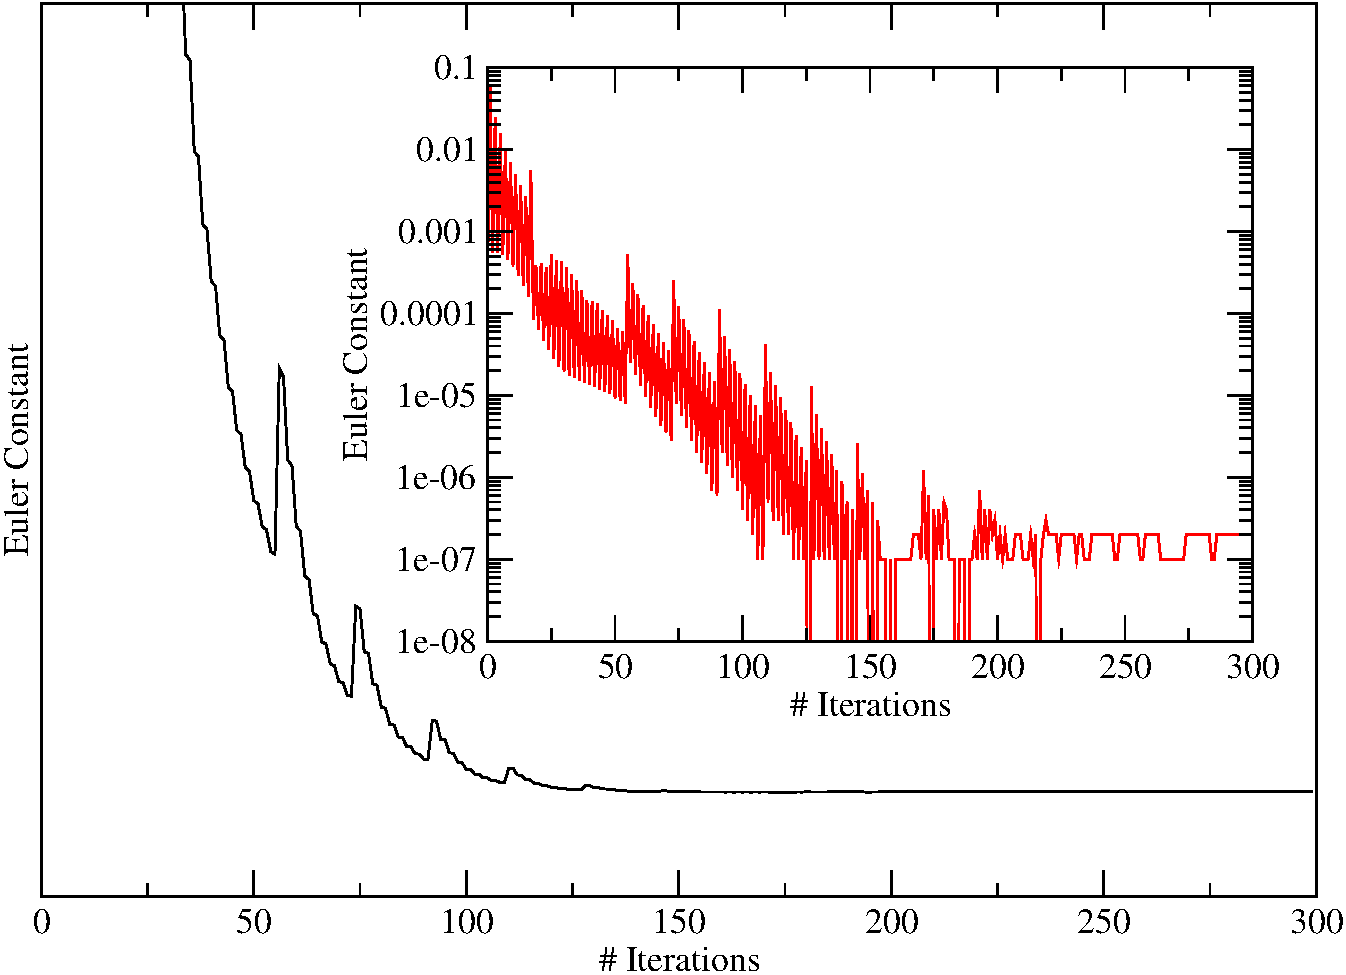
\includegraphics[width=0.95\columnwidth]{Test1} \caption{The
%convergence of the Euler constant as Lev0 iterates.  The inset shows
%the magnitude of the change in Euler constant between neighboring
%iterations.}  \end{figure}









%\item Fig4 of F08 has convergence $J_{BH}$, $P_x$ and $P_y$ as Lev0
%  iterates. We could certainly do the $P_x$ and $P_y$. Probably best
%  to leave out discussion of spin for another part of the
%  paper.\red{This is now shown in figures 3 and 4} \begin{figure}
%  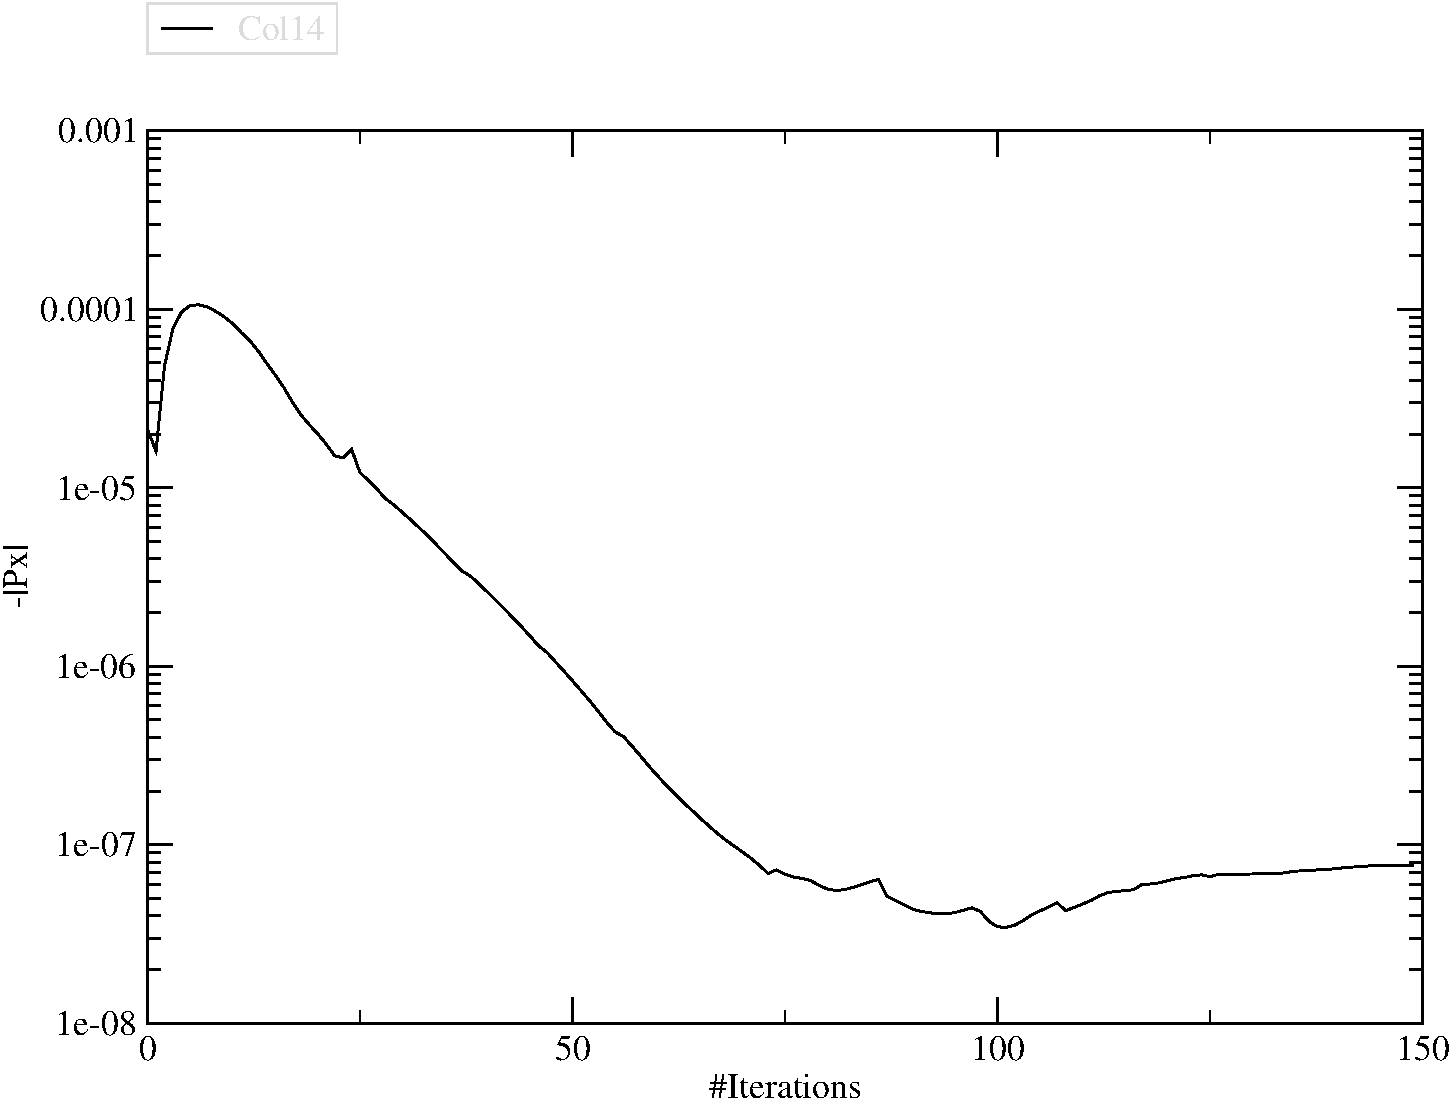
\includegraphics[width=0.95\columnwidth]{Test2_2} \caption{The
%  convergence of the x component of the ADM momentum as Lev0
%  iterates} \end{figure} \begin{figure}
%  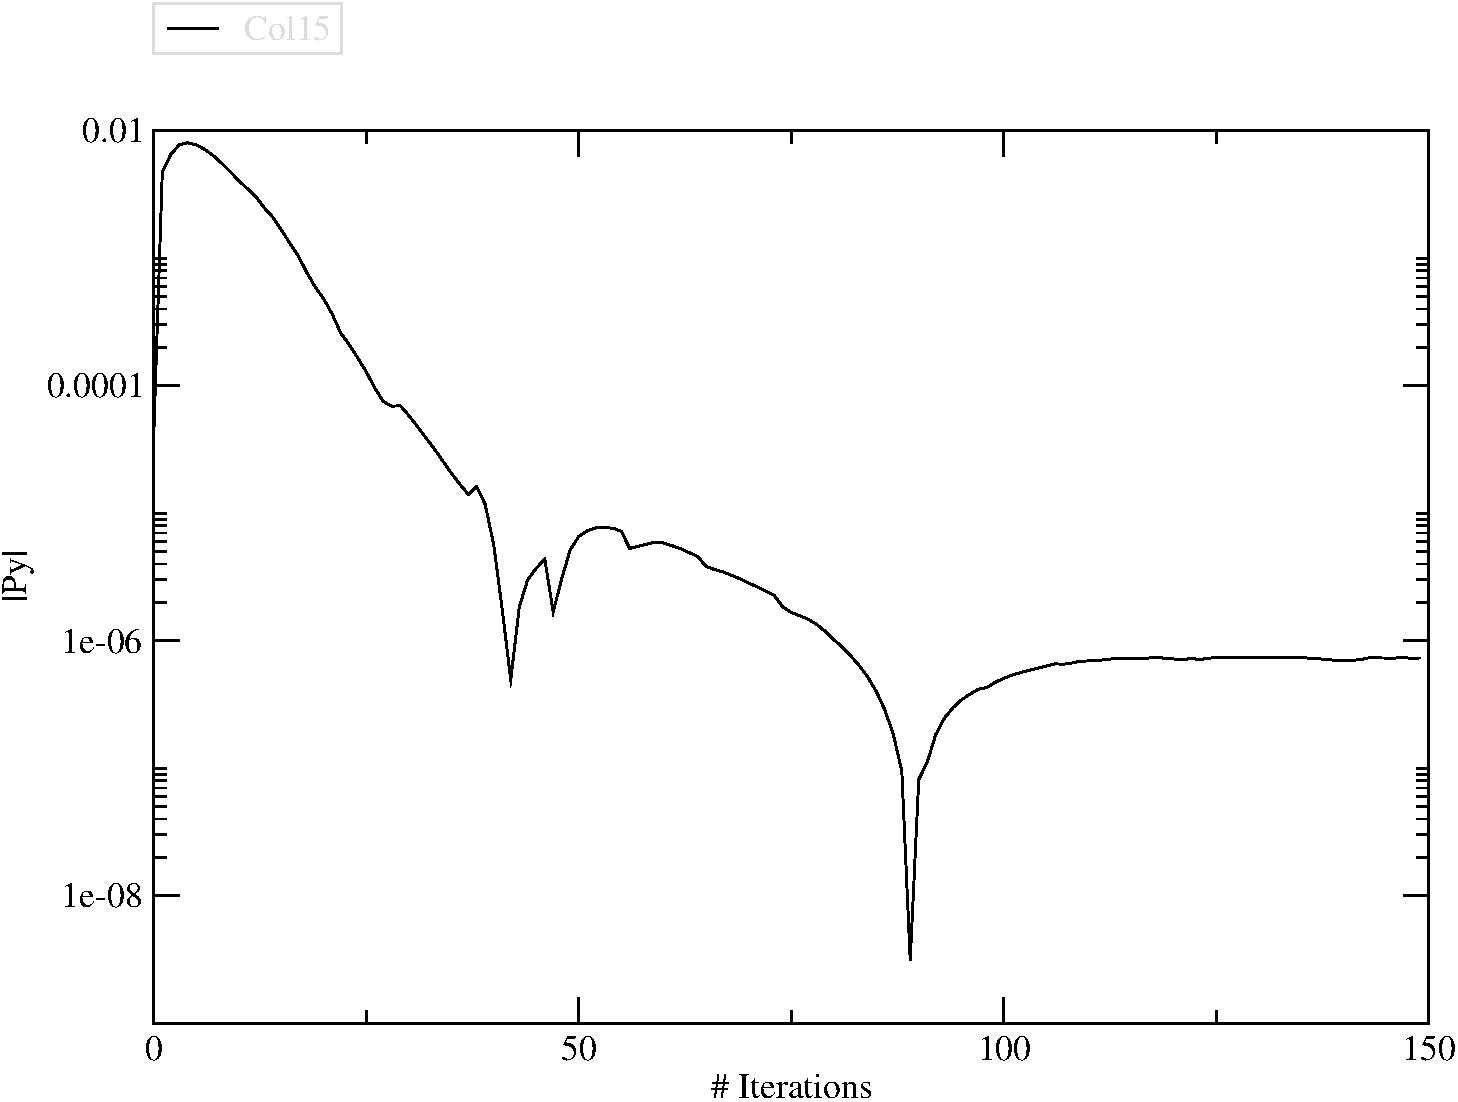
\includegraphics[width=0.95\columnwidth]{Test3} \caption{The
%  convergence of the y component of the ADM momentum as Lev0
%  iterates} \end{figure}


%\item Fig5 of F08 has convergence fo the Ham and Mom constraints
%  versus $N^{1/3}$. This could certainly be done. \red{This is now
%  shown in figures 5 and 6} \begin{figure}
%  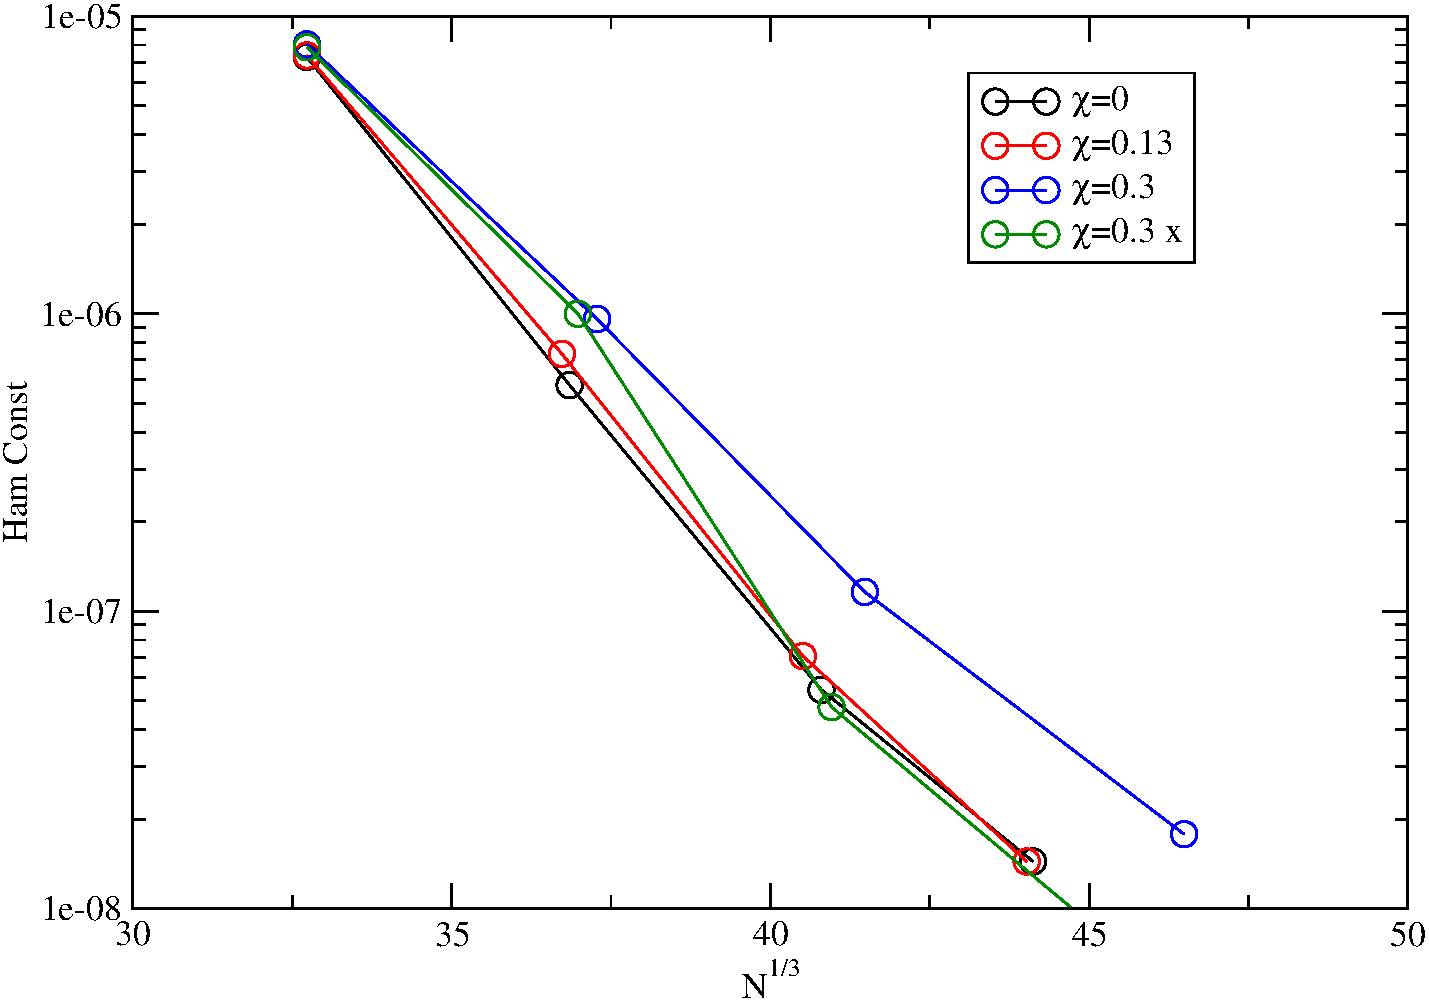
\includegraphics[width=0.95\columnwidth]{Test4} \caption{The
%  convergence of the Hamiltonian
%  constraint} \end{figure} \begin{figure}
%  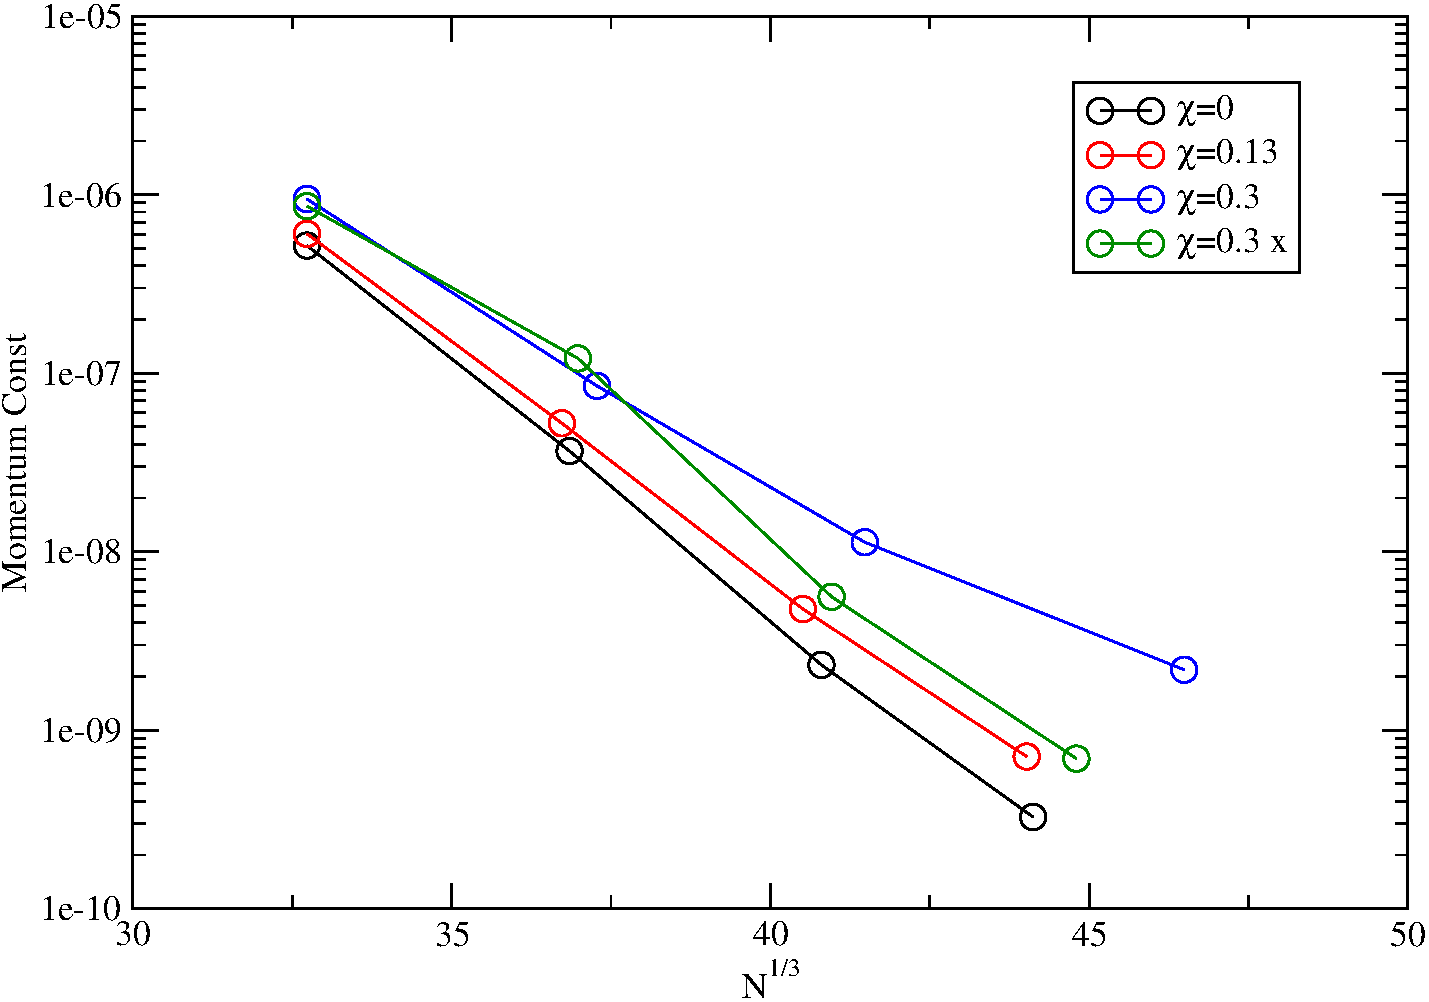
\includegraphics[width=0.95\columnwidth]{Test5} \caption{The
%  convergence of the Momentum constraint} \end{figure}


%\item Fig6 of F08 has ``Convergence of the surface fitting method
%  measured as the evolution of the error in the coefficients of
%  $R_{surf}$ in spherical harmonics, computed here as the difference
%  with our results at our highest resolution''. This seems like it
%  would be useful. Not sure where that data is stored in the ID runs.
%  \red{This is now shown in figure 7} \begin{figure}
%  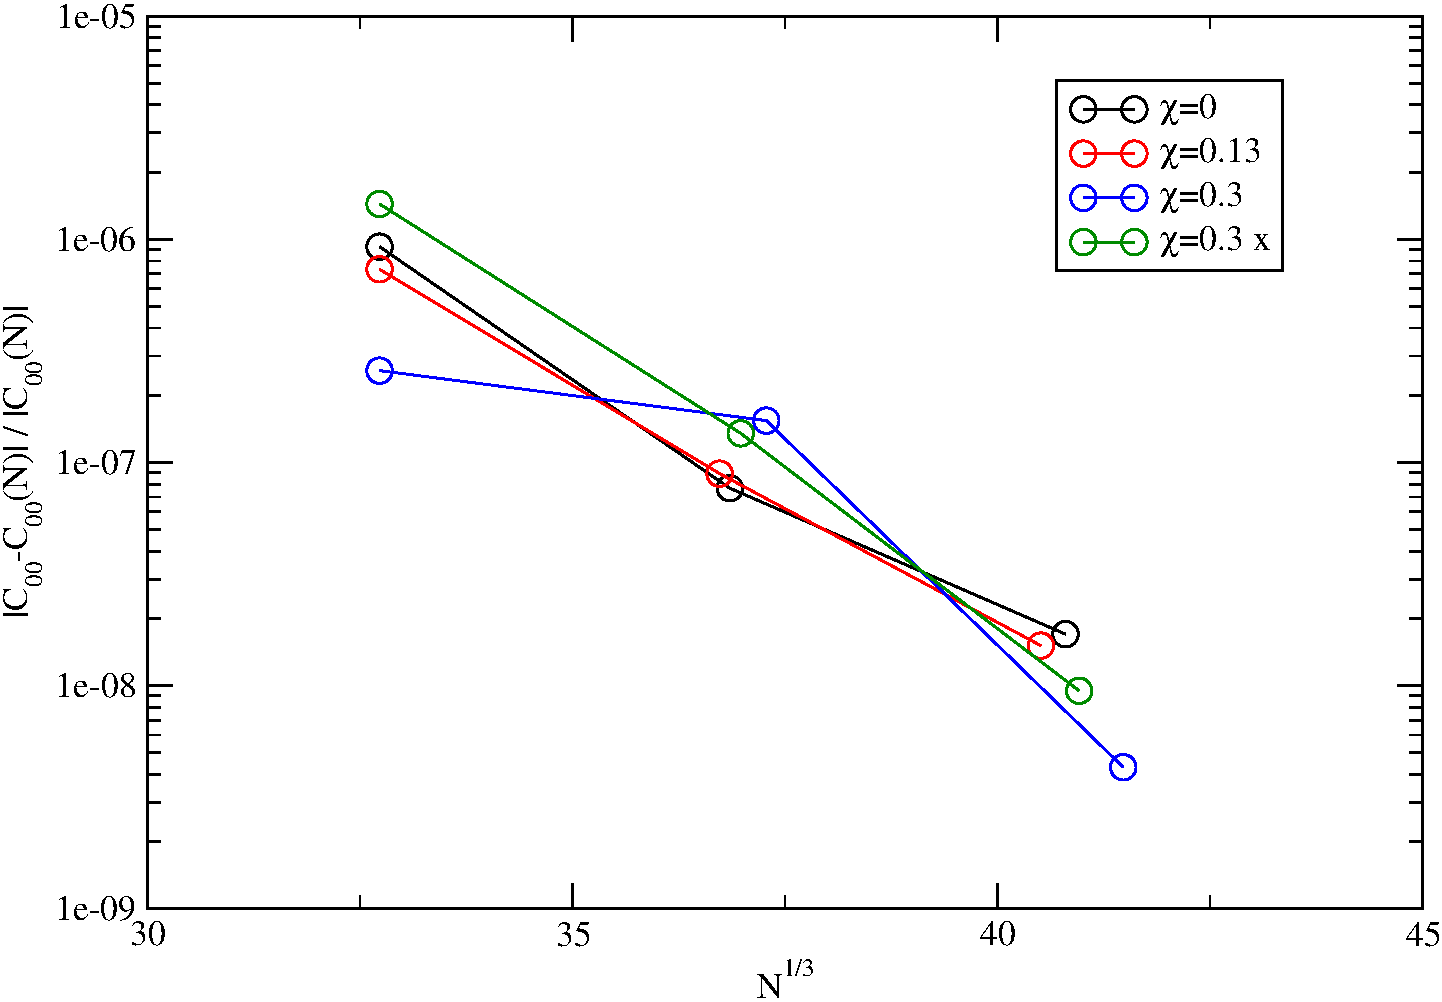
\includegraphics[width=0.95\columnwidth]{Test6} \caption{Convergence
%  of the surface fitting - $\left|1 -
%  \frac{c_{00}}{c_{00}(N)}\right|$, where $N$ refers to the highest
%  resolution, and $c_{00}$ is the l=0, m=0 component of the spherical
%  harmonic decomposition of the surface finder. A more useful
%  quantity will probably involve a sum over the the l,m modes - this
%  needs to be coded in the future} \end{figure}

%\item Fig7 of FO8 has Convergence of ADM energy, ADM angular
%  momentum, difference between Komar and ADM energies and position of
%  the centre of the BH with resolution. These could all be plotted,
%  except for the last. Would convergence of the centre of the NS be a
%  useful quantity to plot? \red{This is now shown in figures 8, 9,
%  10, 11}.

%\begin{figure}
%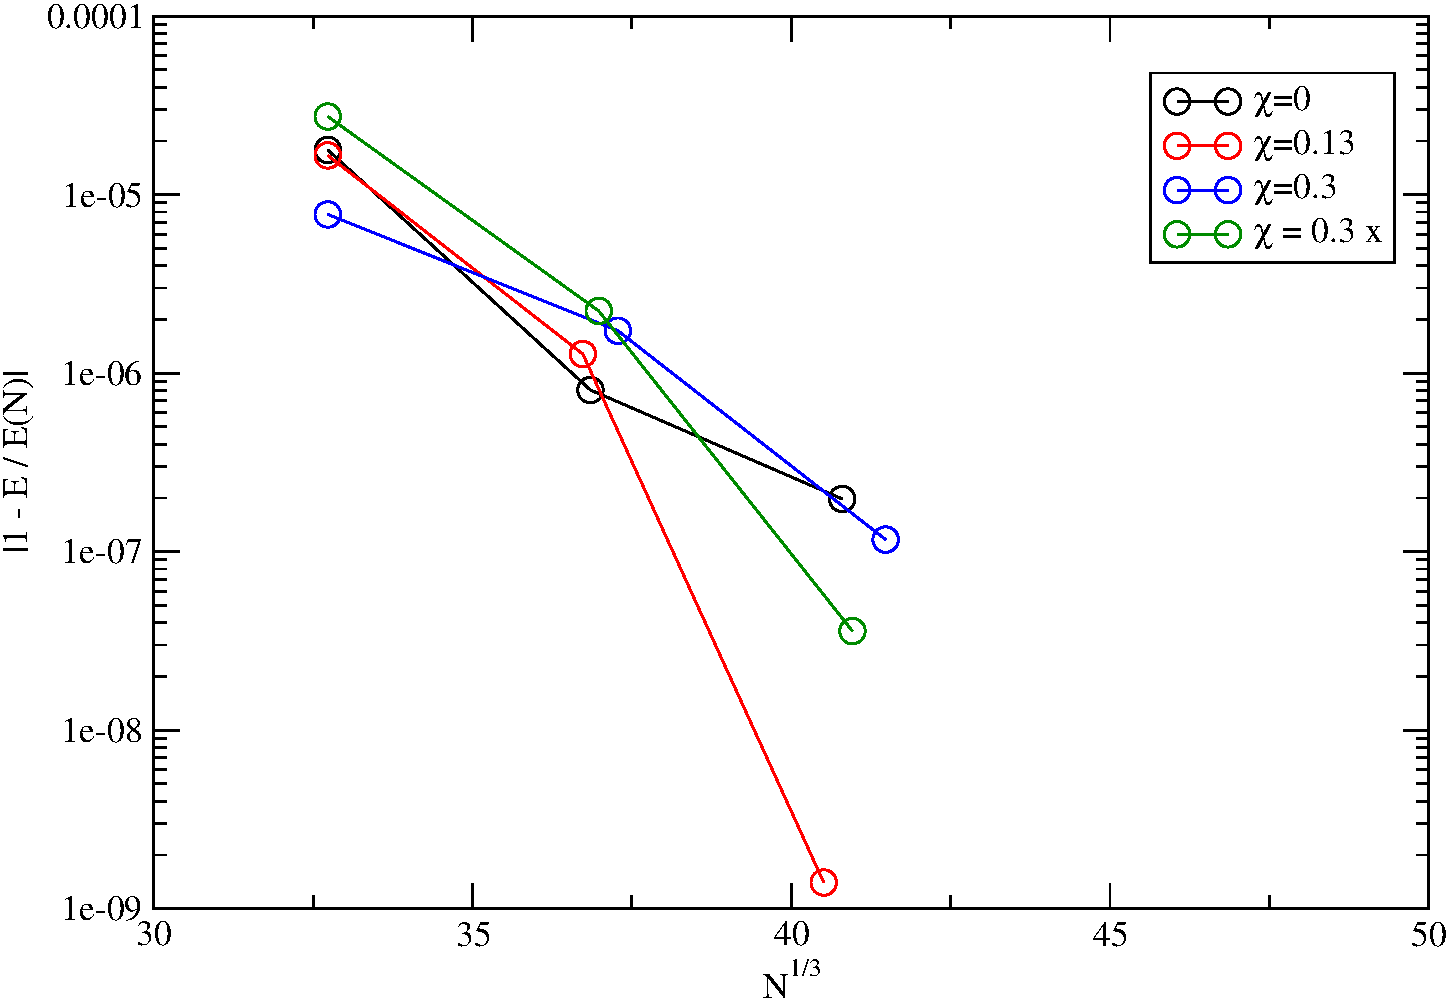
\includegraphics[width=0.95\columnwidth]{Test7} \caption{Convergence
%of the ADM Energy $\left|1 - \frac{E}{E(N)}\right|$ where $N$ refers
%to the highest resolution.}  \end{figure}

%\begin{figure}
%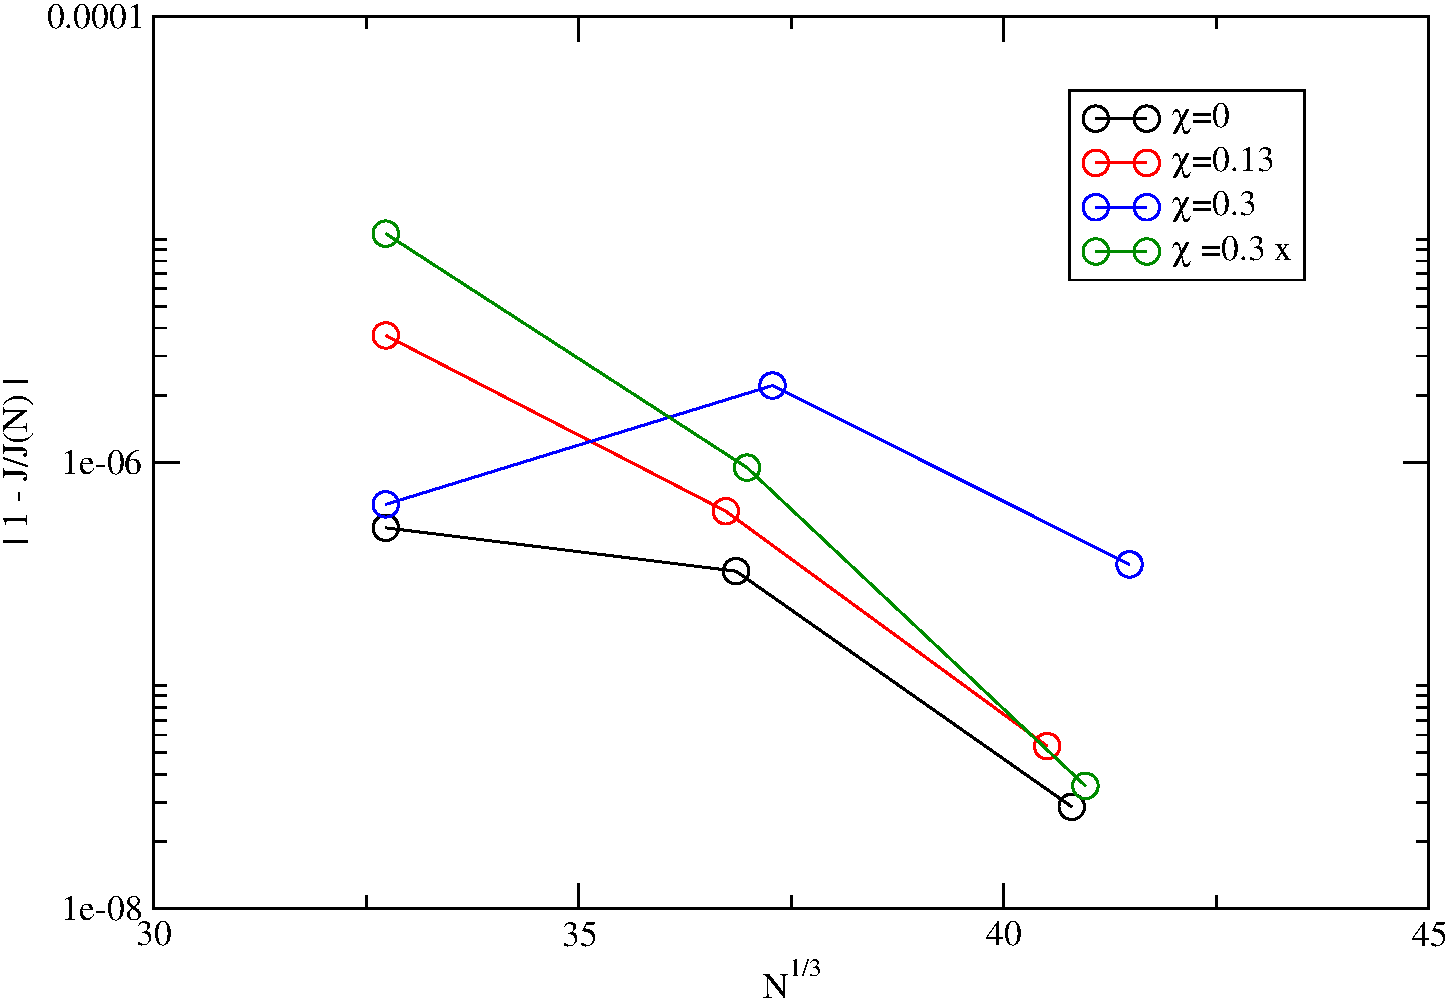
\includegraphics[width=0.95\columnwidth]{Test8} \caption{Convergence
%of the ADM Angular Momentum $\left|1 - \frac{J}{J(N)}\right|$ where
%$N$ refers to the highest resolution.}  \end{figure}

%\begin{figure}
%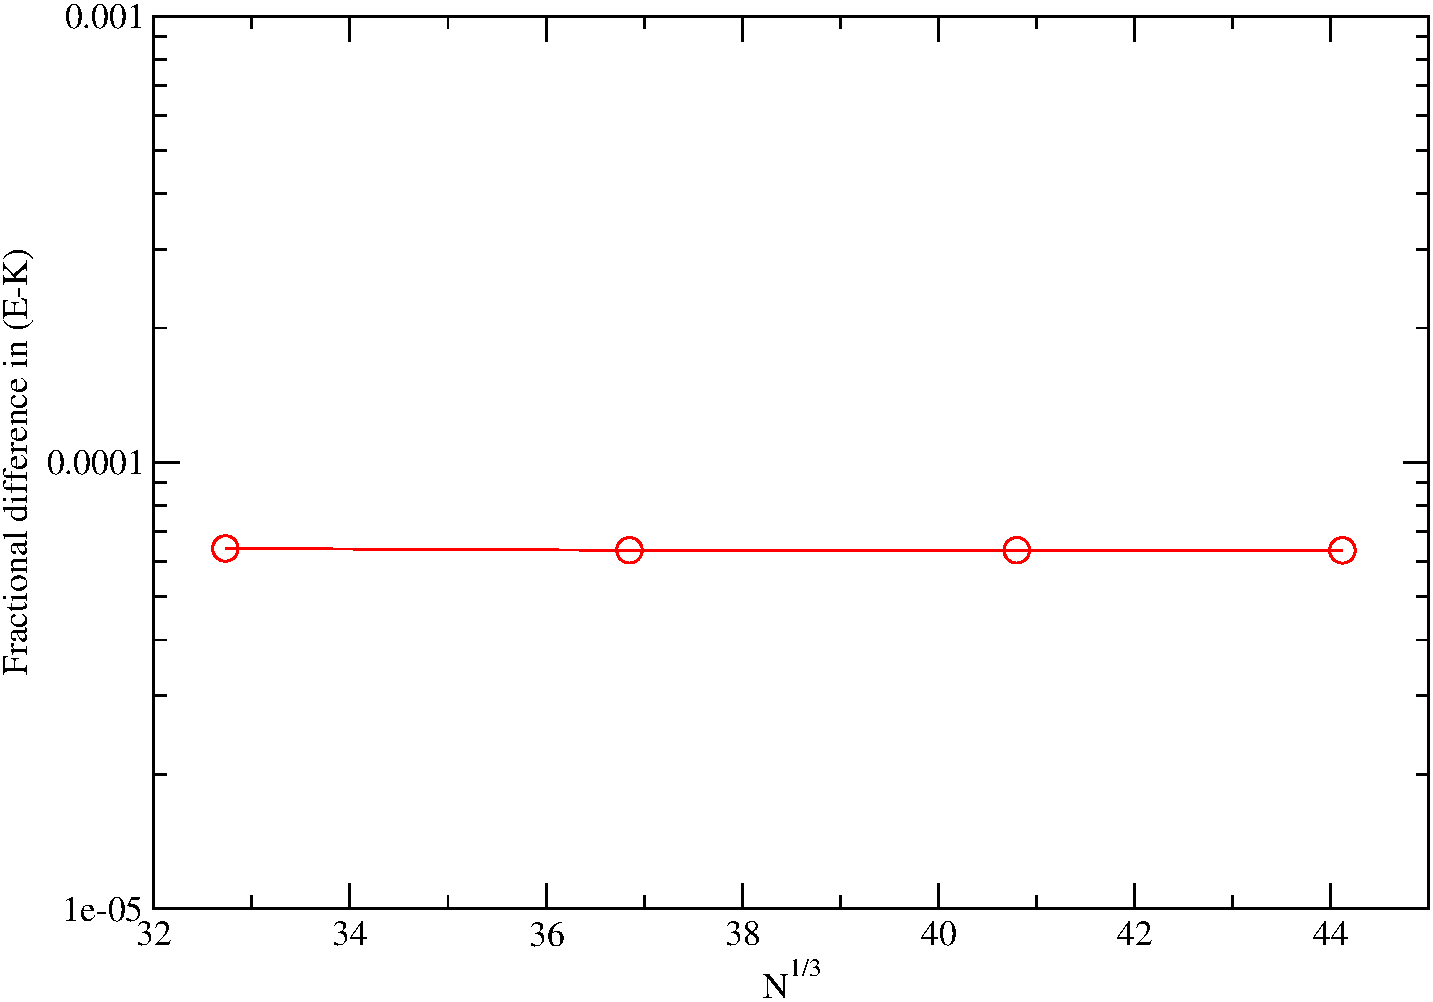
\includegraphics[width=0.95\columnwidth]{Test9} \caption{Convergence
%of the difference between the ADM Energy and the Komar Mass. Not much
%convergence here at all. Is this worth putting in the paper /
%discussing in the paper?}  \end{figure}

%\begin{figure}
%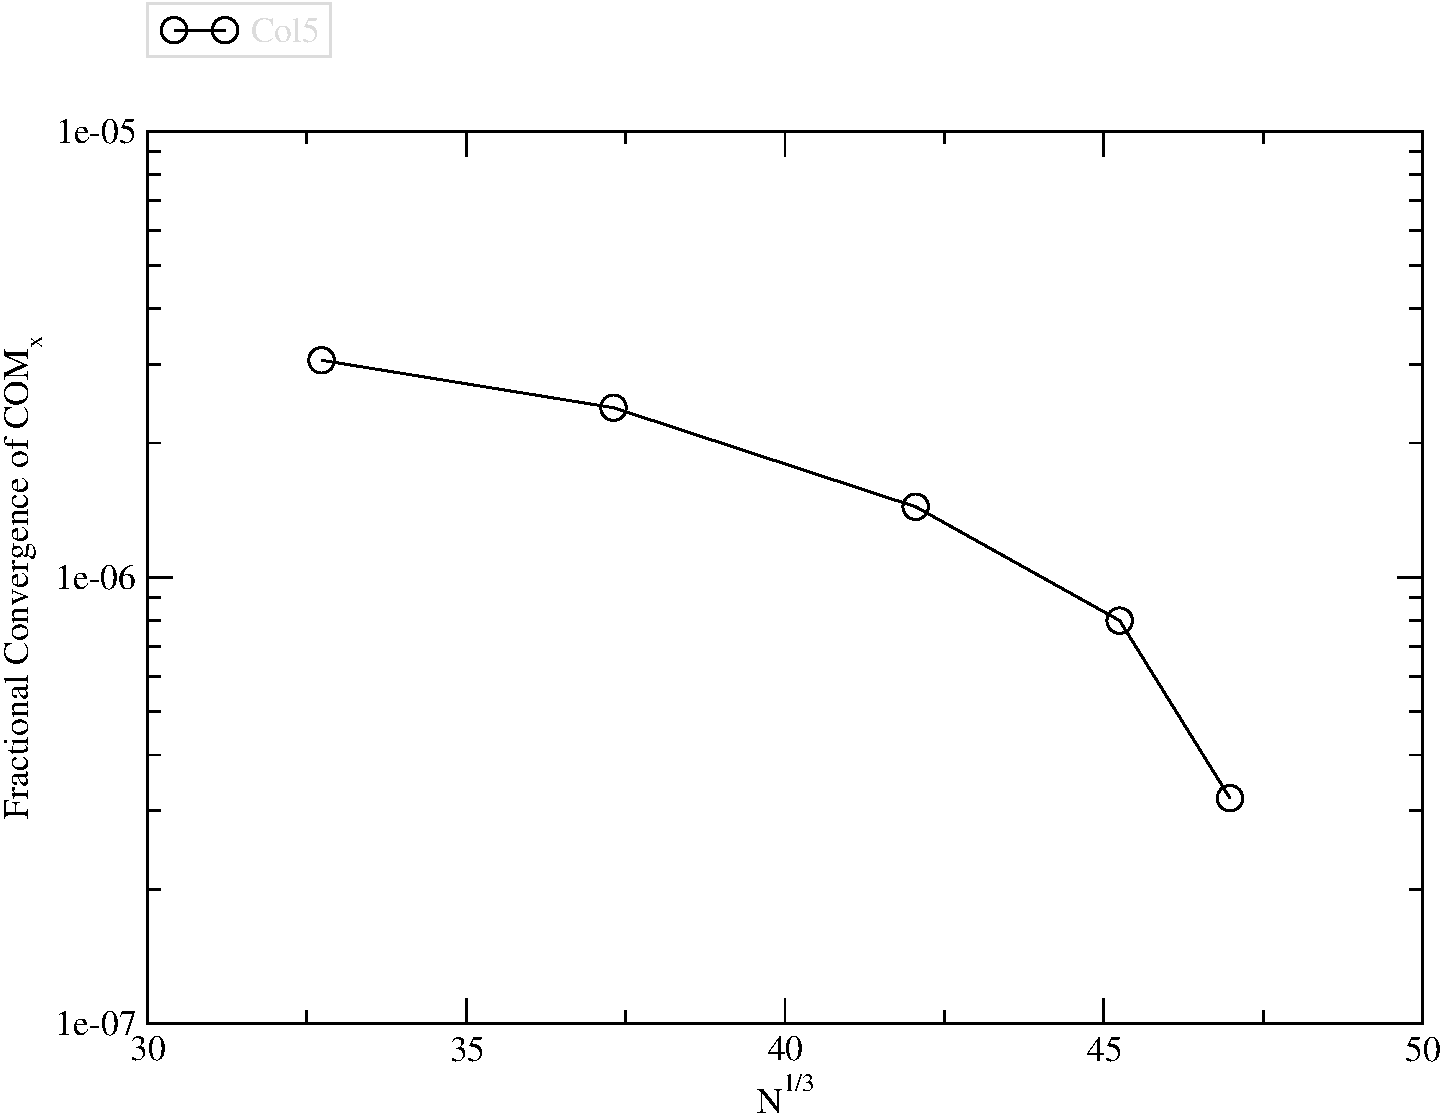
\includegraphics[width=0.95\columnwidth]{Test10} \caption{Convergence
%of the x component of one of the stars' centre of mass. \red{Note:
%This currently shows old data. It needs to be re-run outputting more
%sigfigs to make this plot right!}}  \end{figure}


\subsection{Convergence of the quasi-local spin}

\begin{figure}
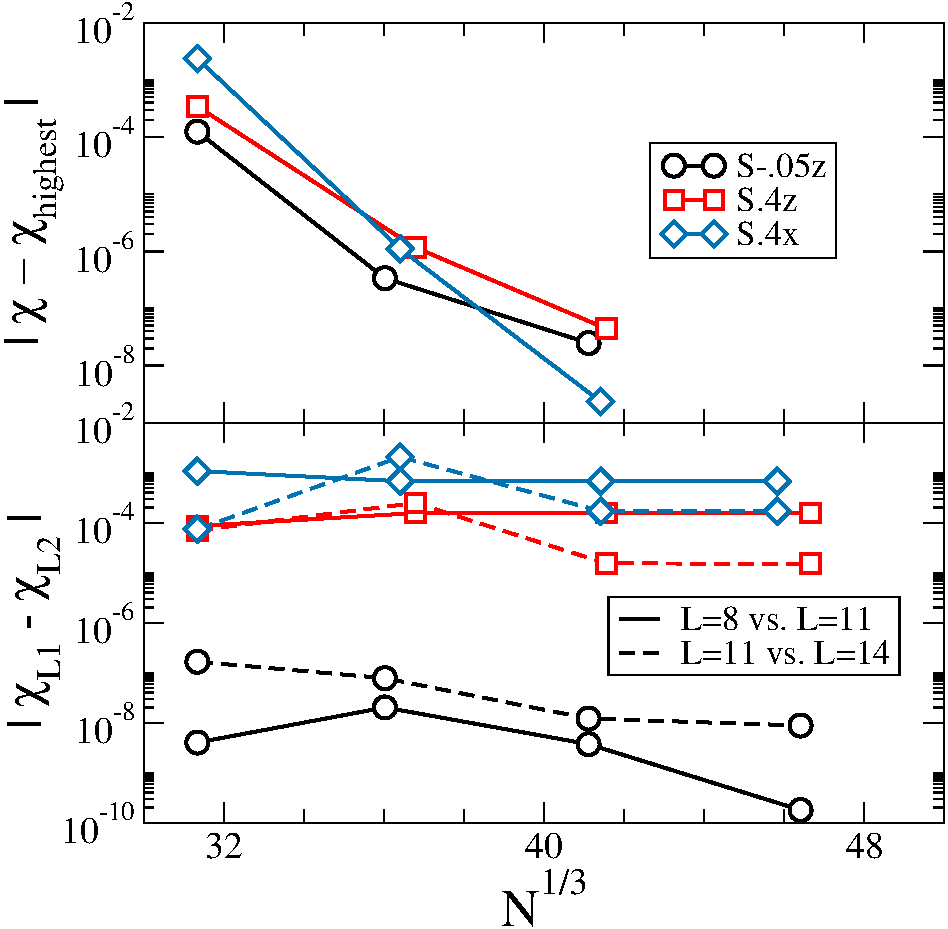
\includegraphics[width=0.95\columnwidth]{SpinConvergence}\\
%\vspace*{-4.5cm}
%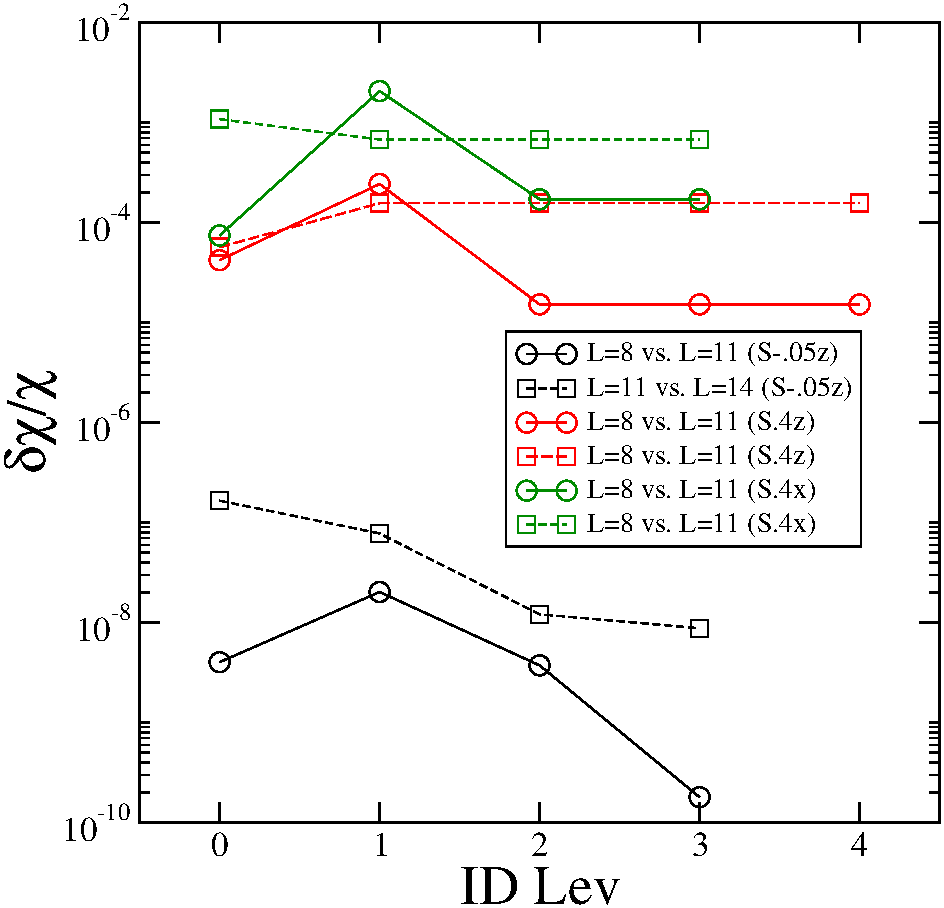
\includegraphics[width=0.4\columnwidth]{LComparison}\vspace{.6cm}

\caption{\label{fig:SpinConvergence} Convergence of the quasi-local
  spin computation.  {\bf Top panel:} difference of spin computed at
  resolution $N$ with the spin computed at the highest resolution.
  {\bf Bottom panel:} Difference between spins computed at different
  resolution $L$ of the spin-computation.  For S-.5z, we achieve an
  accuracy of $\sim 10^{-7}$, whereas for S.4z and S.4x, the
  accuracy is $\sim 10^{-4}$ due to finite $L$.}
\end{figure}

We now turn to the angulr momentum of the Neutron stars, as measured
with quasi-local angular moemntum integrals on the stellar surface.
We will discuss dimensionless spins $\chi$, which depend on two
distinct numerical resolutions: First, the resolution of the
3-dimensional grid used for solving the initial value equations.  This
resulution is specified in terms of $N$, the total number of
grid-points.  Second, the resolution used when solving the eigenvalue
problem for approximate Killing vectors on the 2-dimensional surface,
as given by $L$, the \harald{expansion order in spherical harmonics of the surface-parameterization $r_S(\theta,\phi)=\sum_{l=0}^L\sum_m r_{lm}Y^{lm}(\theta,\phi)$.}
%\roland{you need to tell me in which expansion this coefficient is retained.
%Which ones are the dropped ones?}
Throughout this paper, we use $L=11$.  The top panel of
Fig.~\ref{fig:SpinConvergence} shows convergence of $\chi$ with
grid-resolution $N$, at fixed $L=11$.  We find near exponential
convergence.

The influence of our choice $L=11$ is examined in the lower panel by
computing the quasi-local spin at lower resolution $L=8$ and at higher
resolution $L=11$.  Changing $L$ impacts $\chi$ by $\sim 10^{-9}$ for
the low-spin case S-.05z, and by $\sim 10^{-4}$ for the high-spin
cases S.4z and S.4x.  While it is expected that the more distorted
stellar surfaces of the high-spin stars, the numerical errors of our
spin measurements are still neglible for our purposes.

 % We will now discuss the convergence of the dimensionless spin
 % measured in the initial data. In our initial data solves, the
 % resolution of the grid increases at each ``level'' of the initial
 % data solve. However, the surface finder, which is used to find the
 % surface of each star (by finding an $h=1$ surface), and therefore the
 % surface used to compute the dimensionless spin, uses a fixed
 % resolution. In our runs of interest, this is always $L=11$. We would
 % like to demonstrate that $\chi$ converges as the resolution of the
 % total grid increases, and that $\chi$ converges as the $L$ used in
 % the initial data increases.In figure~\ref{fig:SpinConvergence}, we
 % plot, as a function of initial data resolution, the quantity
 % $\Delta\chi = \frac{|\chi-\chi(N)}{\chi(N)}$, where $\chi(N)$ is the
 % dimensionless spin measured at the highest resolution in the initial
 % data. $\chi$, in this case, means the magnitude of the dimensionless
 % spin vector. There is an overall convergent trend, and this plot
 % shows agreement at the $10^{-6} - 10^{-7} $level for this
 % quantity. Next, we examine what happens when the resolution used for
 % the star's surface finder is changed.

% Next, we will demonstrate the convergence of the QL spin, with the
% resolution, $L$, of the surface finder. In
% figure~\ref{fig:LComparison}, we plot $\frac{\chi_{11} -
%   \chi_{L}}{\chi{11}}$ as a function of initial data level. Here
% $\chi_{11}$ is the dimensionless spin measured in the usual $L=11$
% initial data, and $\chi_{L}$ is both the spin measured for $L=8$
% initial data (dashed curves) and for $L=14$ initial data (solid
% curves). In all cases, this quantity is lower for $L=14$ than for
% $L=8$, showing that the measured spin is indeed converging with
% increased surface finder resolution. For both of the highly spinning
% cases, this quantity is significantly larger than that plotted in
% figure~\ref{fig:SpinConvergence}, showing that the limited surface
% finder resolution is the dominant source of error. However, we still
% find agreement with $L=14$ at the $10^{-4} - 10^{-5}$ level, which we
% consider acceptable for the present work. For the low-spinning run, we
% find that the error due to the choice $L=11$ is significantly lower,
% as expected because of the more spherical shape of the star.  The
% dominant source of uncertainty here comes from the resolution of the
% grid (cf. Fig.~\ref{fig:SpinConvergence}), although that uncertainty
% is still quite small.


\begin{figure}
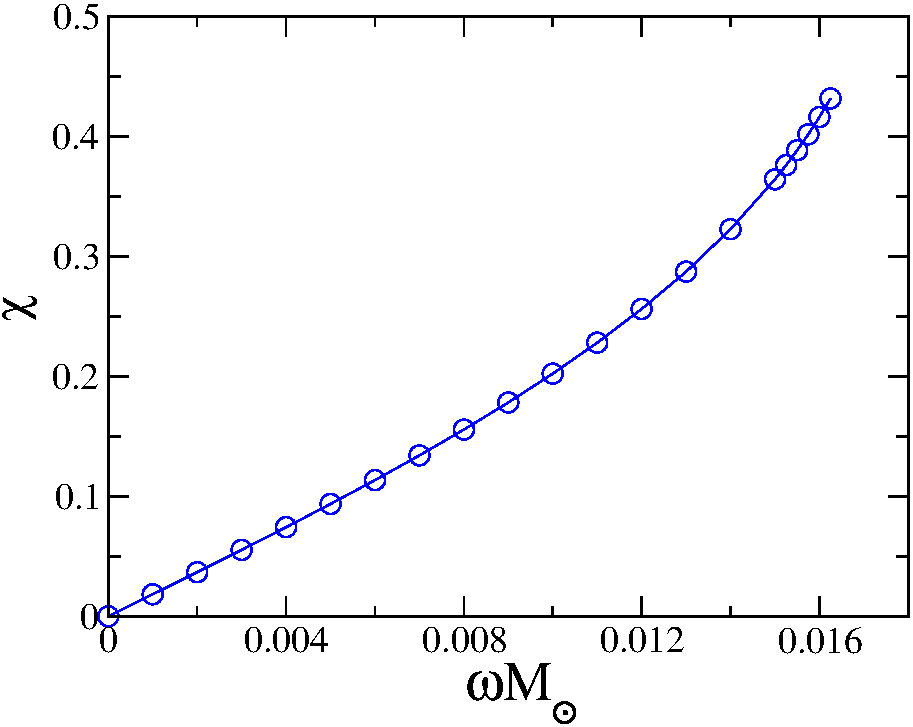
\includegraphics[width=0.95\columnwidth]{ChiVOmega}
\caption{{\label{fig:ChiVOmega}} $\chi$ as a function of $\Omega$ for
  a series of spin-aligned initial data sets with the same physical
  parameters as our runs of interest. We see, as expected, a linear
  relation between $\chi$ and $\Omega$ at low-spins, which eventually
  becomes non-linear at higher spins. }
\end{figure}


%%%%%%%%%%%%%%%%%%%%%%%%%%%%%%%%%%%%%%%%%%%%%%%%%%%%%%%%%%%%%%%%
\subsection{Quasi-local Spin}
\label{sec:QLSpinProperties}
%%%%%%%%%%%%%%%%%%%%%%%%%%%%%%%%%%%%%%%%%%%%%%%%%%%%%%%%%%%%%%%%

As discussed in section~\ref{sec:QLSpinExplanation}, we use a
quasi-local spin to define the angular momentum carried by each
Neutron star.  To our knowledge, this is the first application of this
method to neutron stars in binaries. 
% We will use the symbol
%$\chi=J_{\rm NS} / M_{\rm ADM}^2$ \red{[Refer to definition of
%  $M_{\rm ADM}$]} to represent the dimensionless spin of the neutron
%star - analogous to the quantity more commonly used to discuss the
%spins of black holes. In this section, we aim to convince the reader
%that this quantity is both reasonable and robust, by showing that it
In this section, we explore properties of the rotating NS-NS initial datasets and the employed quasi-local spin diagnostic.
%acts in a physiccally reasonable way, and that it converges in a
%meaningful sense.

To explore the spin-dependence of NS-NS initial data sets, we
construct a sequence of equal-mass, equal-spin NS-NS binaries, with
spins parallel to the orbital angular momentum.  We fix the initial
data parameters $M^b_{\rm NS}$, $D_0$, $\Omega_0$ and $\dot{a}_0$ to
their values for S.4z - Ecc1 (cf. Tab.~\ref{tab:ecc_removal}), and vary the
magnitude of $\bm\omega$.  Figure~\ref{fig:ChiVOmega} presents the
dimensionless spin of either Neutron star as a function of $\omega$.
$\chi$ increases monotonically with the rotation parameter $\omega$.
For $\omega=0$, the quasi-local spin of the Neutron stars is
$\chi=2\times 10^{-4}$.  The spin $\chi$ increases linearly with
$\omega$ for small $\omega$.  For larger $\omega$, the dependence
steepens, as the increasing equatorial radius of the stars increase
the moment of inertia~\cite{Worley:2008cb}.  For $\omega=0.01625$, we
achieve $\chi=0.438$, the largest spin we are able to construct.  This
is reasonably close to the theoretical maximum value for $\Gamma=2$
polytropes, $\chi\sim 0.57$~\cite{Ansorg:2003br}.  Above
$\omega=0.01625/M_\odot$, the initial data code fails to converge.  The
steepening of the $\chi$ vs. $\omega$ curve is reminiscent of features
related to non-uniqueness of solutions of the extended conformal thin
sandwich equations~\cite{Lovelace2008,Pfeiffer-York:2005,Baumgarte2007,Walsh2007},
and it is possible that the failure to find solutions originates in a
break-down of the uniqueness of solutions of the constraint equations.
Henriksson et al~\cite{Henriksson:2014tba} encountered significant
obstacles when constructing NS initial data for neutron stars with
high compactness.  It is possible that high spin causes shifts
difficuties of the convergence of the iterative procedure to the lower
compactness considered here, causing the failure of our iterative procedure for $\omega>0.01625$.

To continue our examination of the initial data sets, we show in
Fig.~\ref{fig:Bulging} cross-sections through one of the Neutron stars
in the xz-plane, i.e. a plane orthogonal to the orbital plane which is
intersecting the centers of both stars.  With increasing $\chi$, the
stars develop an increading equatorial budge.  Both
Figs.~\ref{fig:ChiVOmega} and~\ref{fig:Bulging} indicate that the
initial-data formalism indeed does construct rotating Neutron stars.

%   As a first
% simple check that our stars are acting in a physically reasonable way,
% using the same sets of initial data, we examine cross-sections of the
% stars' surfaces in the X-Z plane. As is well known, spinning bodies
% will bulge at the equator, and bulge more the faster they rotate. As
% the spin axes of these stars is the $+\hat{z}$ direction, we expect
% them to elongate in the $x$ direction and shorten in the $z$
% direction, the faster they rotate. In figure~\ref{fig:Bulging} we plot
% these cross-sections for stars with spins ranging from $\chi=0$ to
% $\chi\sim 0.44$. We indeed see the expected effect. This helps further
% show that our stars are indeed acting like spinning objects.

\begin{figure}
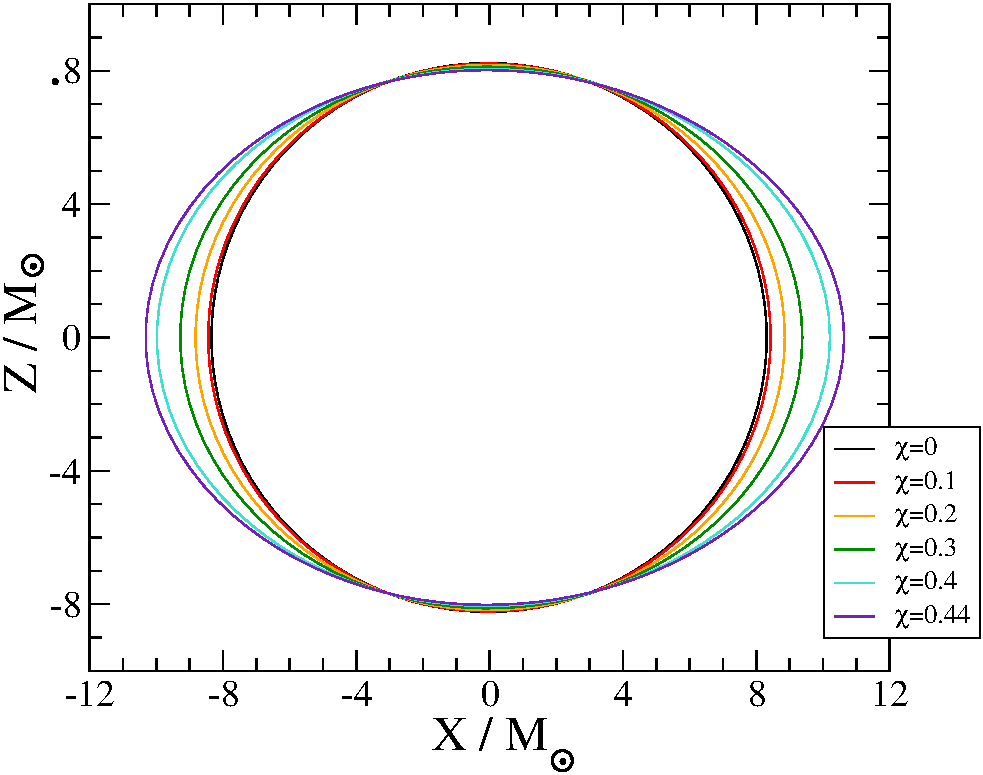
\includegraphics[width=0.98\columnwidth]{Bulging}
\caption{{\label{fig:Bulging}}Stars' surfaces in the X-Z plane for a
  series of different spins, aligned with the $\hat{z}$ axis,
  demonstrating that they bulge at the equator in the expected way
  with increasing spin.}
\end{figure}

% As another check that our spinning NS are acting in a reasonable way,
% we compute a series of spin-aligned initial data with $\omega$ (the
% star's angular velocity parameter) ranging from $0$ to $0.01575 M_{\odot}^{-1}$. We use the same parameters, otherwise, that we use for
% our runs of interest, discussed in
% section~\ref{sec:DescriptionOfRuns}. In figure~\ref{fig:ChiVOmega} we
% plot the measured QL spin, $\chi$, as a function of $\omega$ for these
% initial data. This figure demonstrates several important facts. First,
% it shows that we are able to construct BNS initial data for stars with
% spins as high as $\chi\sim 0.45$. This is reasonably close to the
% theoretical maximum value for $\Gamma=2$ polytropes, $\chi\sim
% 0.55$. Above this value, however, we are unable to find convergent
% solutions. This figures also shows the result that we would expect on
% physical grounds - namely that $\chi$ is linear in $\omega$ at low
% enough spins, and starts to become non-linear in $\omega$ at high
% spins, as additional couplings between the moment of inertia and
% $\omega$ are introduced due to the increased equatorial radius \cite{Worley:2008cb}.  The
% behavior in Fig.~\ref{fig:ChiVOmega} is also reminiscent of the
% results of~\cite{Lovelace2008}, where solutions for spinning black
% holes were found only for angular velocities of the horizon below some
% critical value.

% Finally, this plot serves as a sort of calibration tool - given any
% $\Omega$, it can be translated into the correct $\chi$. This should
% also give close to the correct values for NSs of different masses and
% equations of state, provided the right scaling relations are used.

%In figure 4 we show the stars' surfaces in the X-Z plane for a series
%  of different spins, aligned with the $\hat{z}$ axis. These NSs have
%  the same masses, equations of state, and initial separations as our
%  runs of interest. It is well known that spinning bodies will bulge
%  at the equator more and more the faster they rotate. This is what
%  is seen in figure 4, which demonstrates that, qualitatively, our
%  spinning neutron stars are acting in a physicallly reasonable way.


% \begin{figure}
% 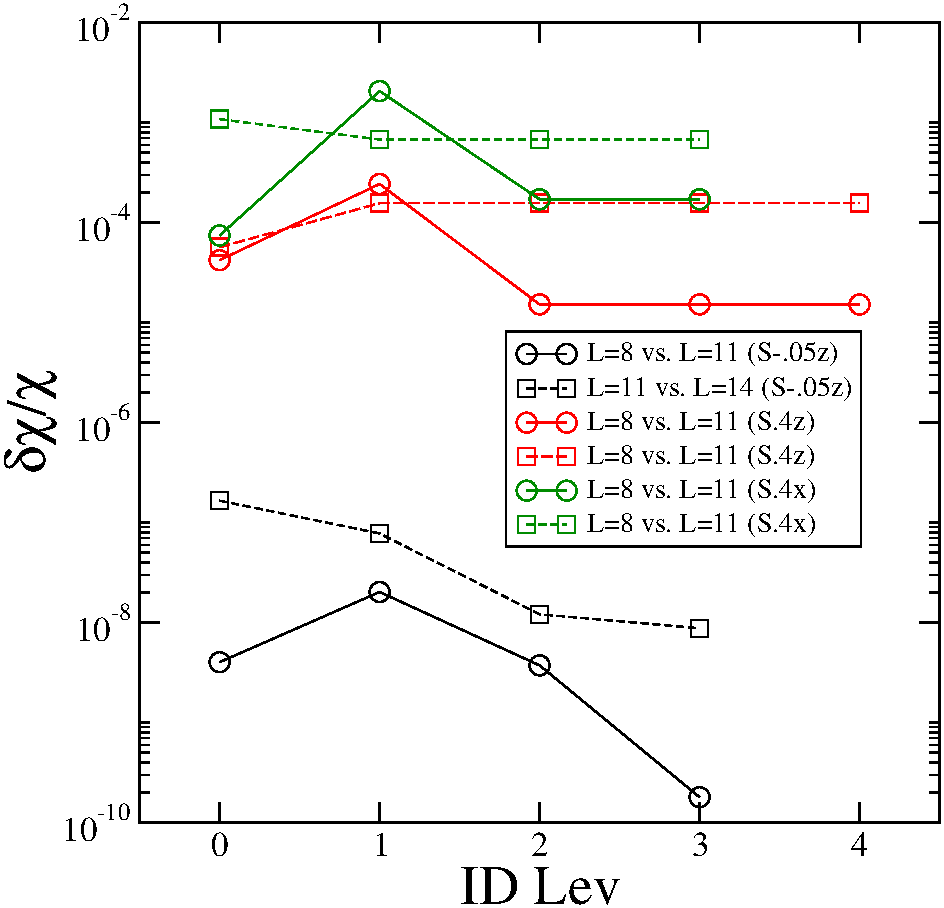
\includegraphics[width=0.5\columnwidth]{LComparison}
% \caption{{\label{fig:LComparison}}Convergence of the dimensionless
%   spin in the initial data, for our three cases of interest, as the
%   resolution of the surface finder goes from $L=8$ to $L=11$ (our
%   usual resolution) to $L=14$. \red{[Incorporate into Fig.~\ref{fig:SpinConvergence}, then remove]} }
% \end{figure}

Finally, we demonstrate that the surface, on which we compute the
quasi-local spin, does not significantly impact the spin we measure:
We choose coordinate spheres centered on the neutron star with radius
$R$, and compute the quasi-local spin using these surfaces,
%  case of measuring the spin on
%spherical shells with radius $R$ 
rather than on the stellar surface.

% For $R<R_{\rm{STAR}}$ we should measure a smaller spin, but
%for $R \geq R_{\rm{STAR}}$ we should measure a comparable spin. 
In Fig.~\ref{fig:ChiVR}, we plot the spin measured $R=\rm{const}$ surfaces, for three
different values of $\omega$, from the sequence shown in Fig.~\ref{fig:ChiVOmega}. 

%In figure 8, we plot $\chi$ as measured on
%spherical shells of radius $R$ for these three cases. 
The circles denote spins extracted on coordinate spheres.  The asterisks
indicate the spins computed on the stellar surface. The asterisk is
plotted at $R=R_{\rm eq}$, the equatorial radius of the neutron star
under consideration.  
%point included on each curve represents $\chi$ as measured using the
%surface finder, and with $R$ equal to the star's equatorial radius. 
We find good agreement between spins extracted on coordinate spheres and
the spin extracted on the stellar surface, as long as $R\ge R_{\rm eq}$. 
 The maximum disagreement is seen in the high spin curve, where
the two spins differ by $\sim 10^{-2}$.  

For $R<R_{\rm eq}$, the coordinate extraction sphere intersects the
outer layers of the neutron star and  does no longer
encompass the entire matter and angular momentum of the star.
Therefore, $\chi(R)$ shows a pronounced decline for $R<R_{\rm eq}$ for
each of the three initial-data sets considered in Fig.~\ref{fig:ChiVR}.
For $R>R_{\rm eq}$, $\chi(R)$ continues to increase slightly, for
instance, for the middle curve, $\chi(R=9)=0.202$ whereas
$\chi(R=11)=0.204$.

In summary, Fig.~\ref{fig:ChiVR} shows that the quasi-local spin
extracted on coordinate spheres can serve as a good approximation of
the quasi-local spin extracted on the stellar surface (as long as the
coordiate sphere is outside the star, of course).
% shows a couple of important
%things. First, it shows that that $\chi$ behaves as a function of $r$
%in the way that we would expect, up to some minor
%differences. Secondly, it shows that measuring the spin on
%$r={\rm const}$ surfaces gives sensible results, as long as
%$r>R_{\rm{star}}$. 
This is important because during evolutions of the
binary, we do not track the surface of the star.
%, as it is too
%computationally inefficient and it is difficult to resolve the
%low-density regions. 
Instead, we will compute the spin on coordinate spheres, similarly to Fig.~\ref{fig:ChiVR}.

\begin{figure}
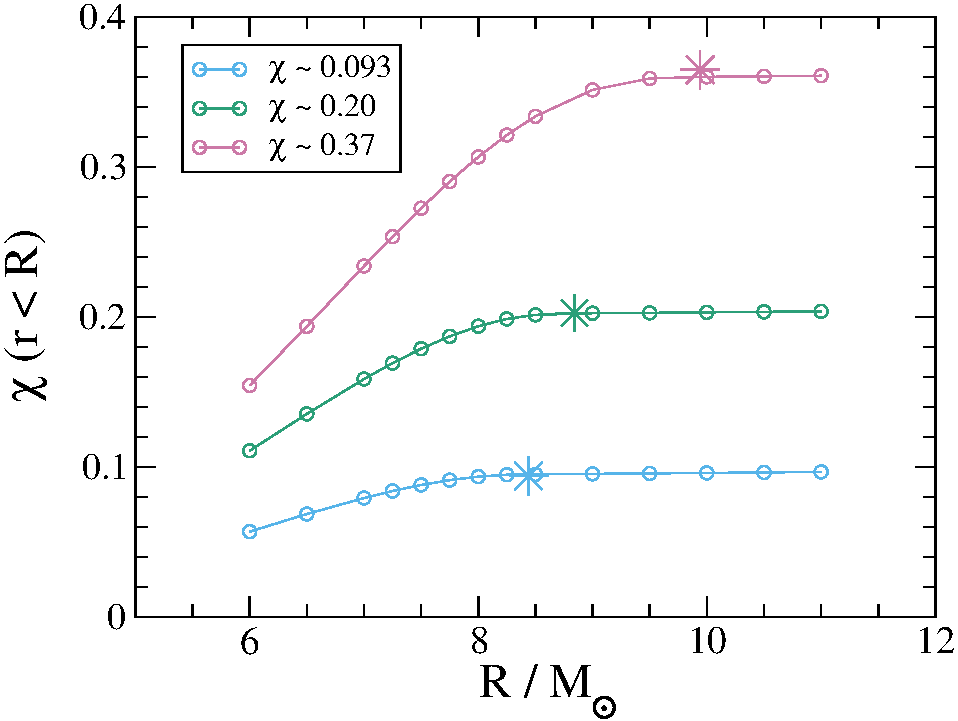
\includegraphics[width=0.95\columnwidth]{ChiVR}
\caption{{\label{fig:ChiVR}}Dimensionless spin $\chi$ measured on
  coordinate spheres with radius $R$ for three different aligned spin
  BNS systems.  The asterik denotes the spin measured on the
  (non-spherical) stellar surface.  Circles to the right of the
  asterik represent coordinate spheres entirely outside the Neutron
  star, and circles on the left of the asterik indicate spin
  measurement surfaces that intersect the star or are entirely located
  inside the star.}
\end{figure}

%\begin{comment}

%\begin{itemize}

% \item \red{Discuss the minor disagreement between the two methods in more detail}
% %\item \green{To include:{Reference describing non-linear behavior of
% %$\chi$ vs. $\Omega$ plot \red{[HP: Lovelace et al.  Perhaps
% %Pfeiffer+York, Baumgarte+OMurchada+Pfeiffer]}}}
% \item \green{To include?: A plot of the stars' velocity fields -
%   showing they look like a uniform rotation}
% \item \green{To include: Discussion of agreement between $\Omega$
%   direction and QL spin direction.}
% %\item \green{To include: A plot showing QL spins converge independent of surface}
% %\item \green{To include: A plot showing QL spin behaves vs. compactness in a reasonable way}
% \item \green{To include?: A plot showing agreement between QL spin and
%   $J_{ADM}$ in the expected way}
% \item \green{To include?: A comparison between corotating star and
%   spinning star.  \red{sounds interesting, but there's already enough
%     material, so optional}}
% \end{itemize}






%A plot of $\chi$ vs. $\Omega$ could be useful, as it can show that
%the QL spin responds in an intuitive way to Orbital frequency (linear
%at low spin, non-linear at high-spin \red{Is there a good reference
%with which to compare the non-linear behaviour?}) and it also
%demonstrates the highest spins we can achieve in the initial
%data. This is now shown in figure 12.

%\begin{figure}
%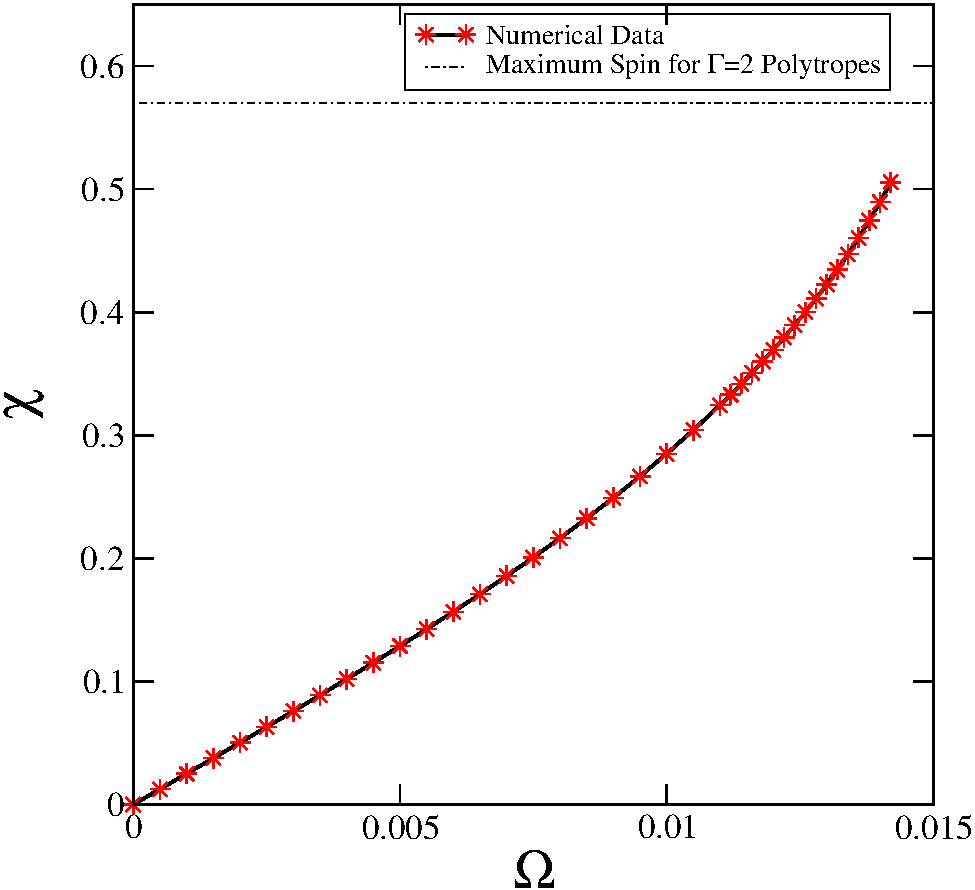
\includegraphics[width=0.95\columnwidth]{JvsOmega} \caption{Neutron
%star dimensionless spin vs. $\Omega$} \end{figure}

%\item A plot of the stars' surface (in the x-z plane) for different
%spins would be useful, as it will show the star bulging as the spin
%increases. This is now shown in figure 13.

%\begin{figure}
%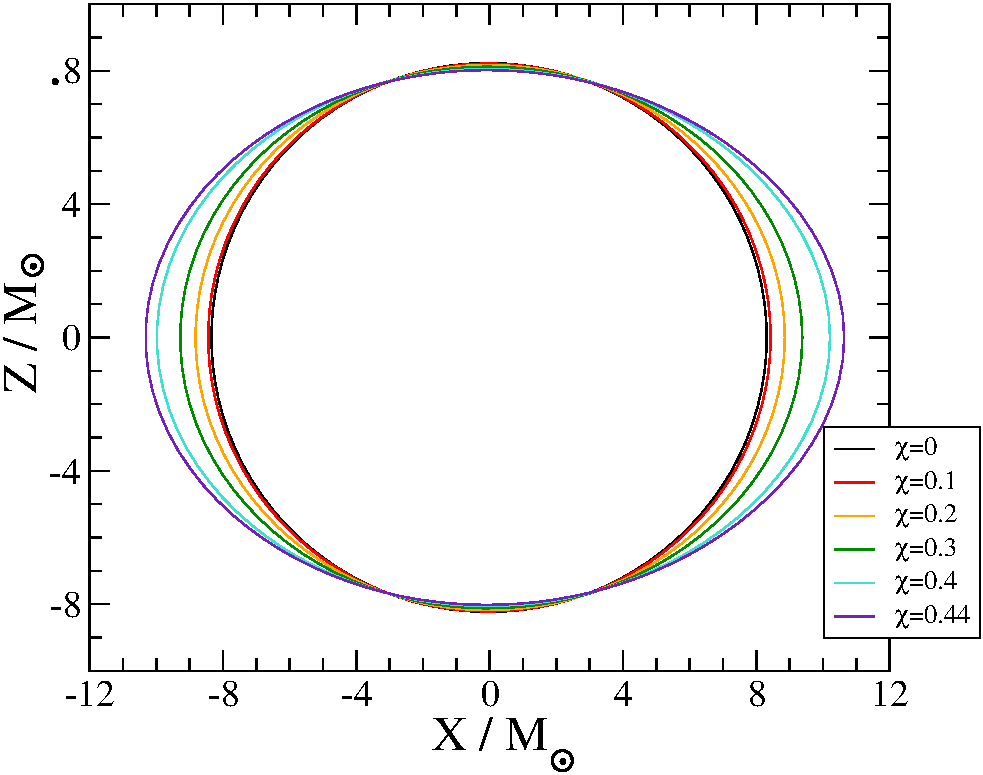
\includegraphics[width=0.95\columnwidth]{Bulging} \caption{Neutron
%stars cross-sections in the x-z plane for 6 different
%spins.}  \end{figure} \red{Other things to show?
%Ideas: \begin{itemize} \item Plot of velocity fields (i.e. does it
%look like a uniform rotation?)  \item Perhaps something like a plot
%of $\theta_{CODE}$ vs. $\theta_{QLSPIN}$ for a number of different
%configurations. Essentially we want to show they agree \item Show QL
%spin converges with resolution in ID solve \item Show QL spin can
%also be measured on spheres (rather than $h$=1 surface) and converges
%to the same value \item Show QL spin behaves in the way you would
%expect for different compactness at constant mass \item Show QL spin
%is equal to the ADM $J$ in the head-on, spin in the x-direction
%case \item Compare star to corotating solution with same/similar
%spin \end{itemize}}

\section{Evolution Results}
\label{sec:EvolutionResults}

%\begin{itemize}
%\item \sout{Description of evolution code}
%\item \sout{More description of runs}
%\item \sout{Orbital hangup in aligned runs}
%\item \sout{Gravitational waves}
%\item \sout{Demonstate ecc removal}
%\item \sout{NS spins during evolution are what we claim}
%\item Demonstrate precession
%\item \red{Precessing GW, Comparison with PN}
%\item \sout{Central density variations} 
%\item \red{Constraints during
%  evolution? Different Resolutions?}
%\end{itemize}

%\subsection{Description of Runs}
%\label{sec:DescriptionOfRuns}

We now evolve the three configurations discussed in Sec.~\ref{sec:ID}.
As indicated in Table~\ref{tab:InitialData}, all three configurations
are equal-mass binaries, with individual ADM masses $M_\star$ (in
isolation) 
%\roland{this definition of ADM mass conflicts with the one used in
%the ID section} 
of $1.64M_{\odot}$ or $1.648M_{\odot}$ at initial
separation of $D=47.2M_\odot$, and using a polytropic equation of
state with $\Gamma=2.0$ and $\kappa=123.6$.  Both stars have equal
spins, and the three configurations differ in spin magnitude and spin
direction.  Configuration S-0.05z has spin-magnitudes $\sim 0.05$
anti-aligned with the orbital angular momentum, and the confiurations
S.4z and S.4x have spin magnitudes near 0.4, along the z-axis and
x-axis, respectively.

% \subsection{Summary of Evolutions}
% In this subection we will briefly describe the parameters and results of our evolutions. These will all be explained in greater detail in the subsequent sections.

%We perform evolutions of three configurations: A highly-spinning
%aligned configuration, S0.4z, a highly-spinning precessing
%configuration, S0.4x, and a slowly-spinning anti-aligned
%configuration, S-0.05z. Each case is equal-mass, equal-spin. For all
%three cases, we perform two iterations of eccentriccity removal (as
%described in section~\ref{sec:EccRemoval}), achieving eccentriccities
%of at least $\lesssim 0.002$ in all cases. The S0.4z and S-0.05z cases
%are run at three resolutions, which we call ``Lev 0/1/2''. The S0.4x
%case is run at Lev0/1 only, as it required greater computational
%resources due to the lost symmetry. The details of these resolutions
%are further explained in section~\ref{sec:EvolutionCode}.  Each case
%is run for $\gtrsim 10$ orbits, into the late-inspiral. We do not,
%however, put any of the cases through merger, although this will be
%the focus of future research. All of these details are summarized in
%table~\ref{tab:RunInfo}.


Each configuration is evolved through $\gtrsim 10$ orbits, into the
late-inspiral.  In this paper we focus on the inspiral of the neutron
stars.  Table~\ref{tab:RunInfo} summarizes parameters for these runs.

\begin{table}
%\begin{center}
\begin{tabular} {c | c | c | c | c | c | c}
Name & $k$ & $e$ & $\vec{\chi}$ & $f_{0}(Hz)$ & $N_{\rm orb}$ & $t_{f}({\rm ms})$ \\ \hline
S.4z & 0,1,2 & $\lesssim 0.001$ & $0.381\hat{z}$ & $167.7$ & $11.8$ & $56.0$ \\ \hline
S-.05z & 0,1,2 & $0.0006$ & $-0.050\hat{z}$ & $165.4$ & $12.5$ & $56.3$ \\ \hline
S.4x & 0,1 & $\lesssim 0.002$ & $0.375\hat{x}$ & $164.8$ & $9.1$ & $45.7$ \\ \hline
\end{tabular}
%\end{center}
\caption{ {\label{tab:RunInfo}} Information about our three evolutions.  $k$ indicates the numerical resolutions on which a simulation is performed, $e$ indicates the smallest achieved orbital eccentricity.  $\vec\chi$ and $f_0$ are the dimensionless spins at $t=0$ and the initial orbital frequency.  Finally, $N_{\rm orb}$ and $t_f$ represent the number of orbits the configuration was evolved for, and the evolution time.}
\end{table}


\subsection{Evolution Code}
\label{sec:EvolutionCode}
%\todo[inline]{Include lots of citations in this section!} 
%\red{Can we cite Roland's paper inprep here?}
%Roland says: you could though, it may be better to cite some of Francois' and
%Matt's papers.
%\red{Make this seem less copy-pasted}

In our evolution code, SpEC~\cite{Buchman:2012dw,Lovelace:2011nu,
Scheel2009,Kidder2000a,Lindblom2006,Scheel2006,Szilagyi:2009qz,Lovelace:2010ne,
Hemberger:2012jz,Ossokine:2013zga}, we used a mixed spectral --
finite-difference approach to solving the
Einstein Field Equations coupled to hydrodynamcis. The equations for the
space-time metric,
$g_{\mu\nu}$ are solved on a spectral grid, while the fluid equations
are solved on a finite difference grid, using a high-resolution
shock-capturing scheme. We use a WENO~\cite{Jiang1996202,Muhlberger2014}
reconstruction method to
reconstruct primitive variables, and an HLL\cite{HLL} Riemann solver to
compute
numerical fluxes at interfaces. Integration is done using a 3rd order
Runge-Kutta method with an adaptive stepsize. We interpolate between
the hydro and spectral grids at the end of each full time step, interpolating
in time to provide data during the Runge-Kutta substeps
(see~\cite{Duez:2008rb,FoucartEtAl:2011,Foucart:2013a} for a more detailed
description of the method).

Each star is contained in a separate cubical finite volume grid that does not
overlap with that of the other star. The sides of the grids
are initially $1.25$ times the stars' diameters. We use
grids that contain $97^3$, $123^3$ and $155^3$ points for resolutions
$k=0,1,2$,
respectively\footnote{For aligned-spin configurations S-.05z and
  S.4z, we take advantage of, and enforce, z-symmetry, which halves
  the number of grid-points along the z-axis.}.  These resolutions
correspond to linear grid-spacing of $340\,\text{m}$, $268\,\text{m}$ and
$213\,\text{m}$
respectively for the S.4z case.  The precessing evolution S.4x uses
similar grid-spacing, whereas the anti-aligned run S-.05z has a
slightly smaller grid-spacing because the stars themselves are
smaller. The region outside the NS but inside the finite volume grid
is filled with a low density atmosphere with
$\rho=10^{-13}M_{\odot}^{-2}$.  The motion of the NSs is monitored by
computing the centroids of the NS mass distributions
%\red{[Give formula]} 
\begin{equation}
\label{eq:centroid}
X^i_{\rm CM} = \int{x^iu^0\rho_0\sqrt{-g^{(4)}}d^3x}
\end{equation}
in each for the grid patches containing a NS.

The grids are rotated and their separation rescaled to keep the centers of
the NS at constant grid-coordinates.  As the physical separation
between the stars decreases, the rescaling of grid-coordinates
therefore causes the size of the stars to increases in
grid-coordinates.  In order to avoid the stellar surfaces to expand
beyond the size of the hydro grids, we monitor the matter flux leaving
the hydro-grid along the x, y, and z-direction.  If this flux is too large
along a certain axis, we expand the grid in that direction. Likewise,
if the matter outflow is very small along a certain axis, we contract
the grid.  This procedure allows us to dynamically choose the optimal
grid-size that limits matter loss to a small, user-specified level.
When changing the size of the hydro grid, the number of grid-points is
kept constant, so this process changes the effective resolution during
the evolution.

%\red{[Explain more clearly how many shells cover the stars themselves,
%  rather than the surrounding vacuum.  I owuld expect that the filled
%  sphere covers only the very innermost part of the star (up to which
%  radius?), and a few of the shells cover the rest of the star (how
%  many of the eight?)]}  
The Einstein field equations are solved on a spectral grid. We typically use
scalar spherical harmonic $Y_{\ell m}$, sine and cosine functions and
Chebyshev as well as Jacobi polynomials to decompose the solution on spheres,
circles and linear directions. In this
spectral grid, the central region of each star is covered by a filled sphere
located at
the center of the star. These have spherical harmonic modes up to
$L = 12+2k$.  The radial basis-functions are one-sided Jacobi
polynomials with $7+k$ collocation points. The filled spheres are
surrounded by eight other spherical shells with the same radial and
angular resolutions. At the start of the evolution,
  the stellar surface is generally located inside the third shell.
The far field region is covered by 20 spherical shells starting at 1.5
times the inital binary separation and going out to 40 times that
separation. These shells have angular resolution $L=9+2k$ and radial
resolution $6+k$.  The region between the innermost shell and the
stars is covered by a set of cylindrical shells and fileld cylinders.

We use generalized harmonic coordinates $x^{\mu}$ such that they satisfy a
wave equation
\begin{equation}
\nabla^{\nu}\nabla_{\nu}x^{\mu} = H^{\mu}
\end{equation}
for some freely-specifiable source function $H^{\mu}$. The initial source function $H^\mu_{\rm initial}$ is determined by the intial data. We then transition to a pure harmonic gauge, $H^{\mu}=0$ by using a transition function, i.e.
\begin{equation}
H^\mu = e^{-\left(t/\tau\right)^4}\; H^\mu_{\rm initial}.
\end{equation}
The timescale $\tau$ is determined by $\tau=2\sqrt{d^3/(2M_\star)}$.
This is slow enough to avoid numerical gauge artifacts in the simulations.

%%%%%%%%%%%%%%%%%%%%%%%%%%%%%%%%%%%%%%%%%%%%%%%%%%%%%%%%%%%%%%%%
\subsection{Eccentricity Removal}
\label{sec:EccRemoval}
%%%%%%%%%%%%%%%%%%%%%%%%%%%%%%%%%%%%%%%%%%%%%%%%%%%%%%%%%%%%%%%%

Gravitatonal wave emission reduces orbital eccentricity rapidly during
a GW-driven inspiral~\cite{PetersMathews1963,Peters1964}.  Therefore
inspiraling binary neutron stars are expected to have essentially
vanishing orbital eccentricity in their late inspiral, unless they
underwent recently dynamical interactions.  Our goal is to model the
non-eccentric inspiral.  In this subsection we demonstrate that we can
indeed control and reduce orbital eccentricty, using the techniques
developed for BH-BH
binaries~\cite{,Pfeiffer-Brown-etal:2007,Boyle2007,Buonanno:2010yk}
and also applied to BH-NS binaries~\cite{FoucartEtAl:2008}.


\begin{figure}
  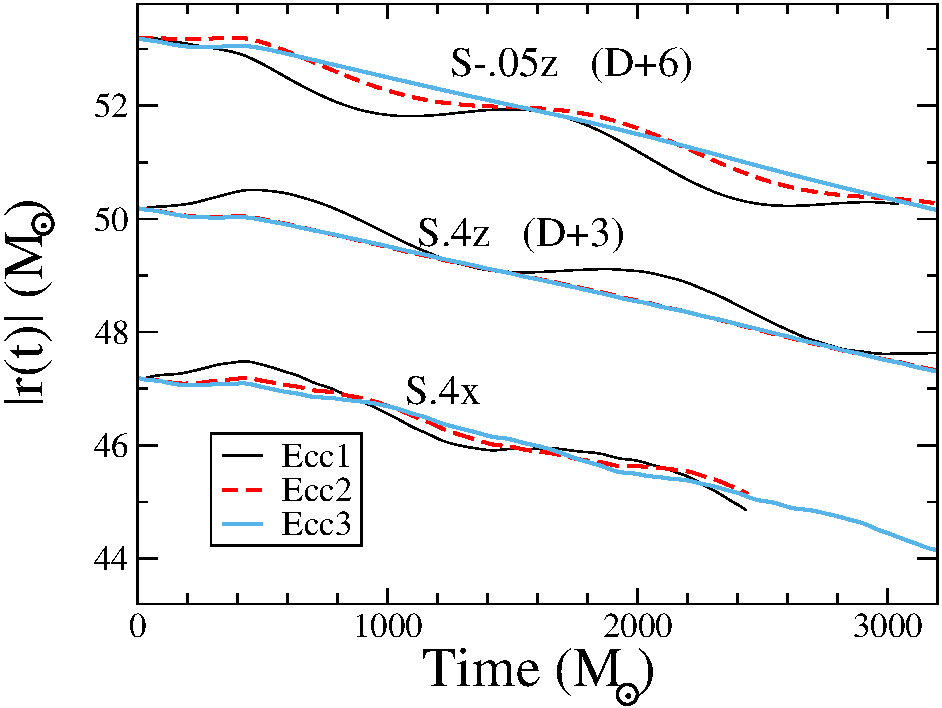
\includegraphics[width=0.95\columnwidth]{DvT2}\caption{{\label{fig:DvT}}The
    binary separation as a function of time.  Shown are three
    eccentricity removal iterations (Ecc1,Ecc2,Ecc3) for each of the
    three configurations studied.  The data for S-.05z and S.4z is
    offset vertically by 6 and 3, respectively, for clarity of
    plotting.}
\end{figure}

% It is well
% known that the orbits of binary compact objects will be nearly
% circular when they are close to merging, and therefore it is important
% to simulate BNS with as low eccentriccity as possible. Here we will
% first describe our algorithm for eccentriccity removal, and then we
% will demonstrate its efficacy for our three runs of interest.

For fixed binary parameters (masses, spins), and fixed initial
separation $D_0$, the initial orbit of the binary is determined by two
remaining parameters: The initial orbital frequency $\Omega_0$, and
the initial radial velocity, which we describe through a expansion
parameter $\dot{a}_0 = \dot{r}/r$.  These two parameters will encode
orbital eccentricty and phase of periastron, and our goal is to
determine these parameters to reduce orbital eccentricity.  We
accomplish this using an iterative procedure \harald{first
introduced for binary black holes~\cite{Boyle2007,Buonanno:2010yk}. An} initial data set
is evolved for a few orbits, the resulting orbital dynamics is
analyzed, and then the initial data parameters $\Omega_0$ and
$\dot a_0$ are adjusted.


\begin{table}
%\begin{center}
\begin{tabular} {l | l | c | c}
Name & $\Omega\times10^{3}$ & $\dot{a}\times10^{5}$ & $e$
\\ \hline S.4z - Ecc1 & $5.10538$ & $0$ & $0.006$ \\ S.4z - Ecc2 &
$5.09591$ & $-1.60$ & $\lesssim 0.001$ \\ S.4z - Ecc3 & $5.09594$ &
$-1.75$ & $\lesssim 0.001$ \\ \hline S-.05z - Ecc1 & $5.10538$ & $0$ &
$0.008$ \\ S-.05z - Ecc2 & $5.11561$ & $0$ & $0.004$ \\ S-.05z - Ecc3
& $5.11769$ & $-1.71$ & $0.0006$ \\\hline S.4x - Ecc1 & $5.10538$ &
$0$ & $0.007$ \\ S.4x - Ecc2 & $5.10429$ & $-2.27$ & $0.004$ \\ S.4x -
Ecc3 & $5.10064$ & $-2.36$ & $\lesssim 0.002$ \\
\end{tabular}
%\end{center}
\caption{\label{tab:ecc_removal} Eccentricity removal for the three
  main runs discussed in this paper.  Only initial orbital frequency
  $\Omega_0$ and initial radial expansion factor $\dot a_0$ are
  changed between different EccN iterations. Recall that these
  quantities have units of $M_{\odot}^{-1}$.}
\end{table}

%%%%%%%%%%%%%%%%%%%%%%%%%%%%%%%%%%%%%%%%%%%%%%%%%%%%%%%%%%%%%%%%
\begin{figure}
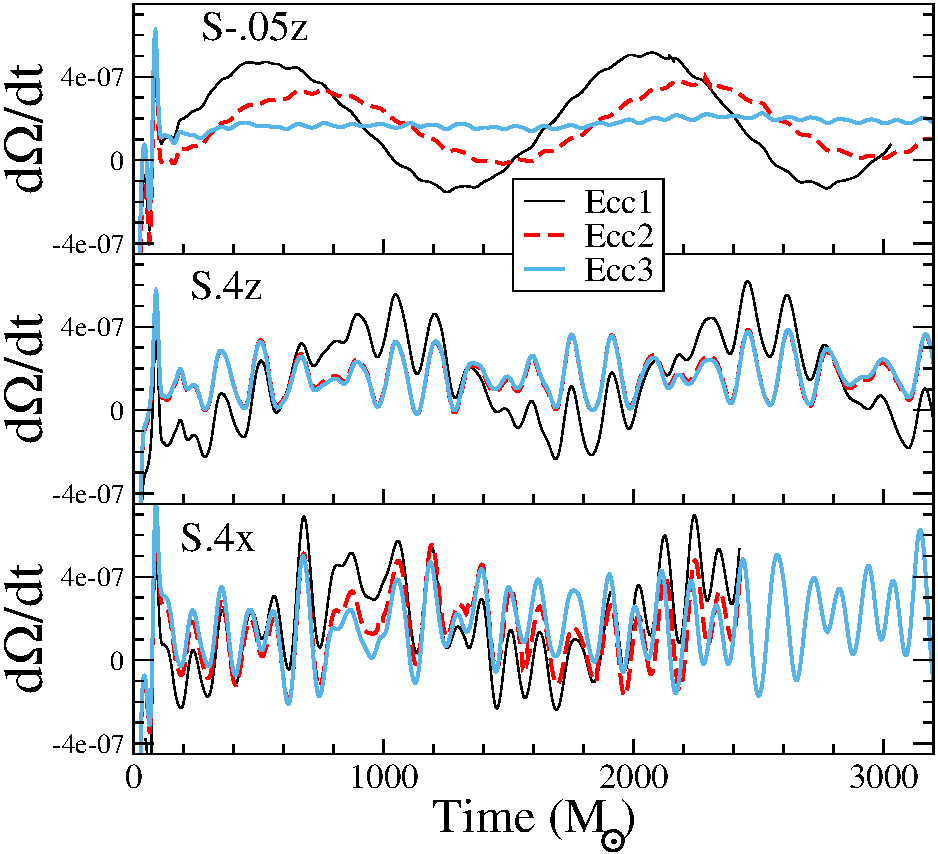
\includegraphics[width=0.95\columnwidth]{DOmegaVT}
\caption{{\label{fig:DOmegaVT}} The derivative of the binary orbital
  frequency as a function of time for different levels of
  eccentriccity reduction for our three runs of interest. }
\end{figure}
%%%%%%%%%%%%%%%%%%%%%%%%%%%%%%%%%%%%%%%%%%%%%%%%%%%%%%%%%%%%%%%%

%For each set of initial data, we must choose an orbital frequency
%($\Omega$) and a radial velocity ($\dot{a}$).  
\harald{For binary neutron stars, we} initialize the first iteration of
  eccentricity removal, \harald{with} $\dot{a}_0=0$ and use $\Omega_0$
  determined from irrotational NS-NS initial data, based on the equilibrium condition in Eq.~\ref{eq:OmegaEq}.  Evolutions
  with these choices are labeled with the suffix ``Ecc1'', and show
  noticable variations in the separation between the two NS, cf. the
  solid black lines in Fig.~\ref{fig:DvT}.
% As we'll show, this still leads to relatively
%low-eccentriccity data, and is therefore perfectly adequate to
%use. After the first run as run sufficiently far (2-3 orbits), we can
%then begin determining the parameters to use for our next level of
%eccentriccity removal. 
We
compute the trajectories of the densest points of each star,
$\vec c_1(t)$ and $\vec c_2(t)$, and using the relative separation
$\vec r=\vec c_2(t) - \vec c_1(t)$, compute the orbital frequency
\begin{equation}
\label{eq:Omega}
\Omega(t) = \frac{|\vec r(t)\times\dot{\vec{r}}(t)|}{r(t)^2},
\end{equation}
where an over-dot indicates a numerical time-derivative.
Finally, we compute $\dot{\Omega}(t)$ and fit it to a function of the form
\begin{align}
\dot{\Omega}(t) = & A_1(t_c-t)^{-11/8} + A_2(t_c-t)^{-13/8}\nonumber \\
&+ B_0\cos{(B_1t
  + B_2t^2 + B_3)}.
\end{align}
The power law parts of this fit represent the orbital decay due to the
emission of gravitational waves, while the oscillatory part represents
the eccentric part of the orbit. We then update $\Omega_0$ and $\dot{a}_0$ 
with the formulae (see
\cite{Buonanno:2010yk} for a detailed overview)
\begin{align}
  \Omega_0 \leftarrow \Omega_0 - \frac{B_0B_1}{4\Omega_0^2}\sin B_3, \\
  \dot{a}_0\leftarrow \dot{a}_0 +\frac{B_0}{2\Omega_0}\cos B_3.
\end{align}
% to determine what
%should be the next ${\Omega}$ and $\dot{a}$. These are chosen such
%that they drive the eccentriccity of an equivalent Newtonian binary to
%0. This process is repeated until the orbital eccentriccity is
%sufficiently low. 
We repeat this procedure twice, resulting in simulations with suffix
Ecc2 and Ecc3.  Table~\ref{tab:ecc_removal} summarizes the orbital
parameters for the individual simulations, and Figs.~\ref{fig:DvT}
and~\ref{fig:DOmegaVT} illustrate the efficiacy of the procedure
through plots of separation and time-derivative of orbital frequency.
The eccentricity is successfully reducued from $e\sim 1\%$ to
$\sim 0.1\%$.  After two eccentricity reduction iterations, variations
in $\dot\Omega(t)$ are so small that they are no longer discernible
within higher-frequency oscillations in $\dot\Omega(t)$,
cf. Fig.~\ref{fig:DOmegaVT}.

%%%%%%%%%%%%%%%%%%%%%%%%%%%%%%%%%%%%%%%%%%%%%%%%%%%%%%%%%%%%%%%%
\begin{figure}
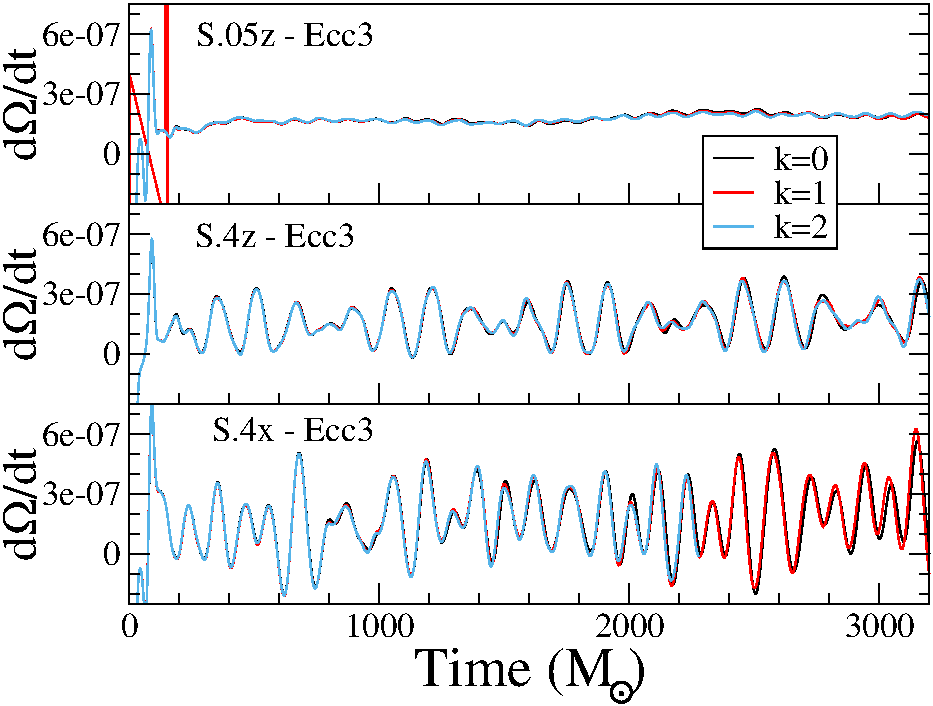
\includegraphics[width=0.92\columnwidth]{OmegaDotComparison}
\caption{ {\label{fig:OmegaDotComparison}Convergence of $\dot\Omega(t)$.  
Shown are $\dot\Omega(t)$  at three different numerical resolutions ($k=0,1,2$) for the
final, lowest-eccentricity initial data.  The oscillations in $\dot\Omega(t)$ are 
evidently not caused by numerical truncation error.}}
\end{figure}
%%%%%%%%%%%%%%%%%%%%%%%%%%%%%%%%%%%%%%%%%%%%%%%%%%%%%%%%%%%%%%%%

The high freuqency oscillations in $\dot\Omega(t)$ are caused by the
quasi-normal ringing of the neutron stars, as discussed in detail
below in Sec.~\ref{sec:QNModes}.  Here, we only note that these
oscillations are convergently resolved,
cf. Fig.~\ref{fig:OmegaDotComparison}, and are therefore a genuine
feature of our initial data.  Figure~\ref{fig:OmegaDotComparison} also
confirms that the lowest resolution ($k=0$) gives adequate resolution
for eccentricity removal.

The eccentriccity removal algorithm attempts to isolate variations on
the orbital time-scale as the signature of eccentriccity. For
S.4z-Ecc2, it reports $e=0.0005$ and for S.4z-Ecc3, $e=0.0002$.
However, given the large amplitude of the QN mode ringing, we consider
these estimates unreliable, and therefore quote an upper bound of
0.001 in Table~\ref{tab:ecc_removal}. Similarly, for S.4x-Ecc3, the fitting
reports $e=0.001$, and we quote a conservative upper bound of 0.002.

%Figures~\ref{fig:DvT} and~\ref{fig:DOmegaVT} illustrate
%the eccentriccity removal process. Figure~\ref{fig:DvT}
%shows the binary separation as a function of time for our three runs
%of interest, at all three levels of eccentriccity removal. It is
%immediately apparent from inspection of these curves that the
%eccentriccity is indeed decreasing with iteration (i.e., the
%oscillations are becoming smaller), except for the case of Ecc2 and
%Ecc3 for the S0.4z run, where those two curves lie nearly on top of
%each other. To measure eccentricity, however, the quantity we fit is
%$\dot{\Omega}$ - this is plotted in figure~\ref{fig:DOmegaVT}. What
%becomes apparent is that for both of the high spin runs, this quantity
%is dominated by noise rather than the signal due to
%eccentriccity. 
%This is particularly true for Ecc2 and Ecc3 for S0.4z
%and for Ecc3 for S0.4x. We believe this is due to excited Quasi-Normal
%(QN) modes in the stars. This effect will be discussed in greater
%detail in section~\ref{sec:QNModes}. The eccentriccity removal algorithm attempts to
%isolate the eccentriccity signal, and for S0.4z, it reports an
%eccentriccity of 0.0005 for Ecc2 and 0.0002 for Ecc3. However, given
%the large amplitude of the QN mode ringing, we consider these
%estimates unreliable, and therefore quote only an upper bound of 0.001
%for those eccentriccities. Similarly, for S0.4x, it reports an
%eccentriccity of 0.001 for Ecc3, but we find stating an upper bound of
%0.002 to be more reliable.



%%%%%%%%%%%%%%%%%%%%%%%%%%%%%%%%%%%%%%%%%%%%%%%%%%%%%%%%%%%%%%%%
\subsection{Aligned spin NS-NS evolutions: NS Spin}
\label{sec:EvolutionSpin}
%%%%%%%%%%%%%%%%%%%%%%%%%%%%%%%%%%%%%%%%%%%%%%%%%%%%%%%%%%%%%%%%

In this section, we will discuss the measurement of spins during our
evolutions for the non-precessing cases, S.4z and S-.05z.  Aligned
spin binaries do not precess.  Combined with the low viscosity we
expect the NS spins to stay approximately constant during the
evolutions.  These systems therefore serve as a test on our spin
diagnostics during the evolutions.
In this section, and through the rest of this paper, we always use the
final eccentricity reduction, ``Ecc3''.  For brevity, we will omit the
suffix ``-Ecc3'', and refer to the runs simply as S-.05z, etc.

%%%%%%%%%%%%%%%%%%%%%%%%%%%%%%%%%%%%%%%%%%%%%%%%%%%%%%%%%%%%%%%%
\begin{figure}
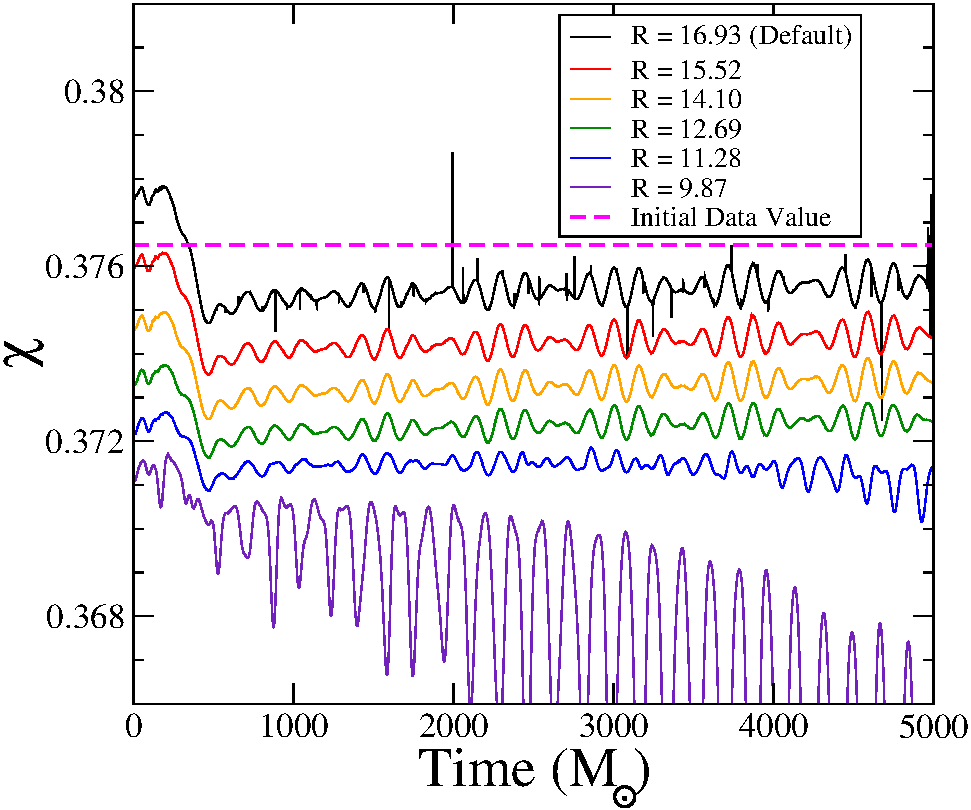
\includegraphics[width=0.95\columnwidth]{ChiVTZoomed}
\caption{{\label{fig:ChiVTZoomed}} The spin measured on multiple
  coordinate spheres for the S.4z run.}
\end{figure}
%%%%%%%%%%%%%%%%%%%%%%%%%%%%%%%%%%%%%%%%%%%%%%%%%%%%%%%%%%%%%%%%

We do not track the surface of the star during the evolution.
%, as the outflow of low-density material at the surface of the star would
%make it too computationally costly \red{[Check - NT]}.
Instead we simply evaluate the quasi-local spin of the stars on
coordinate spheres in the frame comoving with the binary.  We must
therefore verify that the spin measured is largely independent of the
radius of the sphere, and that it is maintained during the evolutions
at the value consistent with that in the initial data.
Figure~\ref{fig:ChiVR} established that coordinate spheres can be used
to extract the quasi-local spin in the initial data.
Figure~\ref{fig:ChiVTZoomed} shows the results for the high-spin
simulation S.4x during the inspiral.

%%%%%%%%%%%%%%%%%%%%%%%%%%%%%%%%%%%%%%%%%%%%%%%%%%%%%%%%%%%%%%%%
\begin{figure}
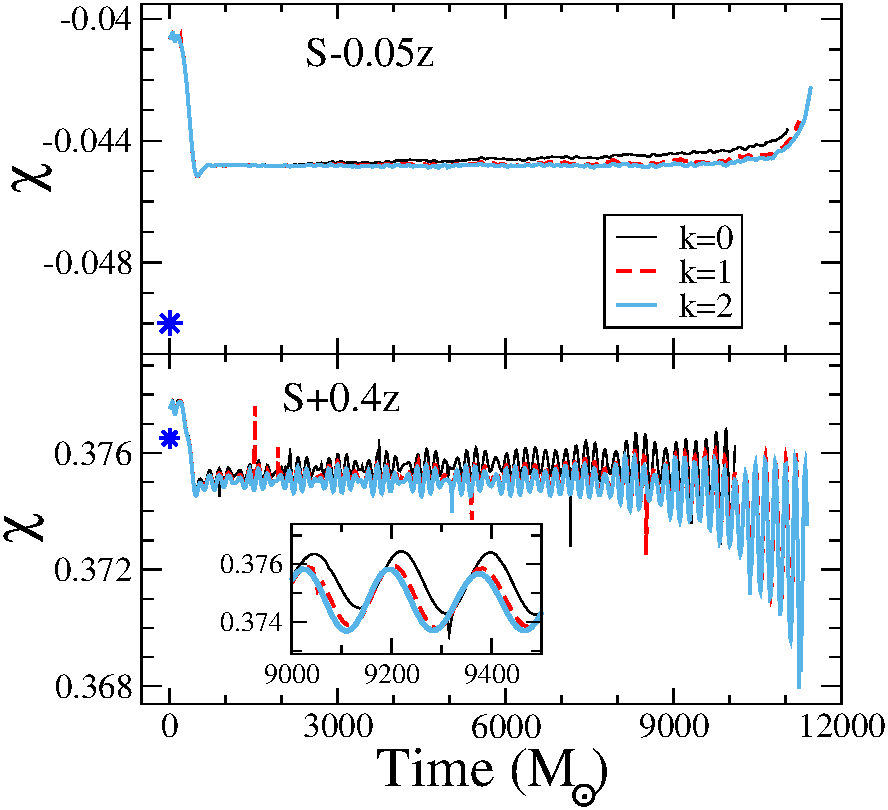
\includegraphics[width=0.99\columnwidth]{ChiVTDifferentRes2}
\caption{{\label{fig:ChiVTDifferentRes2}} Neutron star spin during the
two aligned-spin evolutions.  Shown are three different numerical resolutions, $k=0$ (lowest), $k=1$, and $k=2$ (highest). The asterisk indicates the spin measured on the stellar surface in the initial data.}
\end{figure}
%%%%%%%%%%%%%%%%%%%%%%%%%%%%%%%%%%%%%%%%%%%%%%%%%%%%%%%%%%%%%%%%

For coordinate spheres with radii $R=11.28M_\odot$ to $R=16.93M_\odot$ in grid coordinates, the spins remain roughly
constant in time.  The different extraction spheres yield spins that
agree to about 1\%, with a consistent trend that larger extraction
spheres result in slightly larger spins (as already observed in the
initial data).  The horizontal dashed line in
Fig.~\ref{fig:ChiVTZoomed} indicates the spin measured on the stellar
surface (i.e. not on a coordinate sphere) in the
initial data.  We thus find very good agreement between all spin measurements, and conclude that the quasi-local spin is reliable to about 1\%. 

The extraction sphere $R=9.87M_\odot$ in Fig.~\ref{fig:ChiVTZoomed}
intersects the outer layers of the Neutron star.  Because the
quasi-local spin captures only the angular momentum within the
extraction sphere, the value measured on $R=9.87M_\odot$ falls as our
comoving grid-coordinates cause this coordinate sphere to slowly move
deeper into the interior of the star.  This behavior, again, is
consistent with Fig.~\ref{fig:ChiVR}.

These tests of using multiple coordinate spheres were only run for
about half of the inspiral -- enough to establish that the method is
robust.  Subsequently, we report spins measured on the largest
coordinate sphere, $R=16.93M_\odot$.

The full behavior of the spin during the inspiral is shown in
figure~\ref{fig:ChiVTDifferentRes2} for both the S.4z and S-.05z runs.
Comparing the spin at different resolutions, we note that the data for
$k\!=\!1$ and $k\!=\!2$ are much closer to each other than compared to
$k\!=\!0$, indicating numerical convergence.  We note that the impact
of numerical resolution (as shown in
Fig.~\ref{fig:ChiVTDifferentRes2}) is small compared to the
uncertainty inherent from the choice of extraction sphere,
cf. Fig.~\ref{fig:ChiVTZoomed}.  We also note that for the first
$10000M_{\odot}$ of the run, the measured spin behaves as a constant,
as expected, albeit with some small oscillations. However, toward the
end of the data, we notice the absolute value of the spin start to
decrease in both cases.  

%\harald{\sout{This could be a sign that the extraction
%sphere is becoming too small towards the end of the
%evolution. Whatever the cause, the data after $\sim 10000M_{\odot}$
%seems unreliable.}} \red{[The spin-decrease might also be physical.  In BBH binaries, spin drops due to tidal heating (aka tidal friction).  Compare to aligned spin BBH from the catalog.  Unless we know better what's going on, let's be quiet]}
 
Finally, we note that in both cases, the spin measured in the inital
data on the stellar surface is smaller by about $0.008$ compared to
the evolution.  This difference might indicate the amount of orbital angular momentum stored within the spin extraction sphere.

%Finally, we notice in the S-0.05z case, the
%agreement with the initial data value of the spin magnitude is only
%about 10\%. When the spin is this small, compared to the other two
%cases, a constant error will be magnified in significance.


%\begin{itemize} \item Before discussing the spins we measure during
%our evolutions, we must demonstrate that they are sensible. During
%the evolution we no longer track the surface of the star, so instead
%we measure them on coordinate spheres in the comoving frame. We must
%verify that the spin measured is largely independent of radius, that
%it is maintained as expected for aligned runs during the evolution,
%and that it is agreement with the spin expected from the initial
%data. In figure~\ref{fig:ChiVT} we plot the spin during the evolution
%for our S04z run, at the Ecc3 level. The spin is measured on several
%coordinate sphere of radius $R$. We see that the spins at large
%enough $R$ agree well, while the spins measured at smaller $R$ do not
%incorporate the full star and thus disagree. In
%figure~\ref{fig:ChiVTZoomed} we plot a zoomed-in version of
%figure~\ref{fig:ChiVT}. We can see that the spins agree at the
%fractional level of $\sim \times 10^{-2}$. This is congruent with the
%limitations we claimed in the initial data. We also see that
%agreement with the value measured in the inital data is reasonably
%good.

%\begin{figure}
%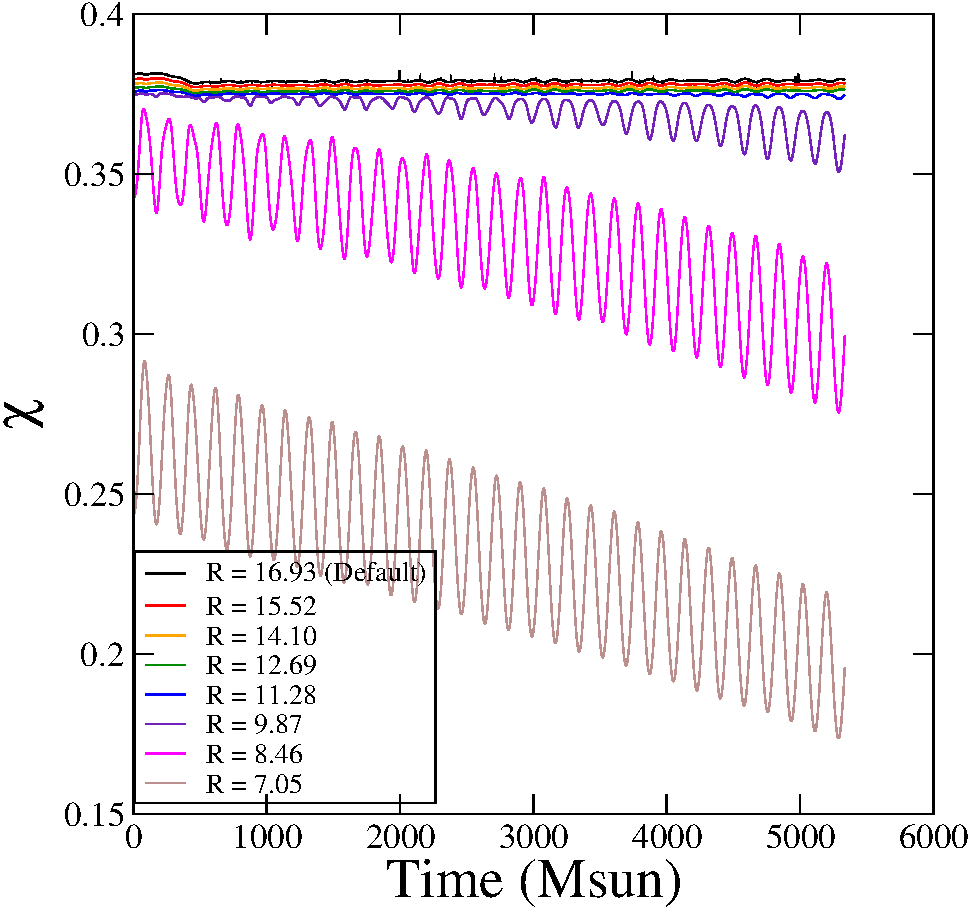
\includegraphics[width=0.95\columnwidth]{ChiVT} \caption{{\label{fig:ChiVT}}
%The spin measured on multiple coordinate spheres for the run
%S04z-Ecc3 \red{REMOVE}} \end{figure}

%%%%%%%%%%%%%%%%%%%%%%%%%%%%%%%%%%%%%%%%%%%%%%%%%%%%%%%%%%%%%%%%
\begin{figure}
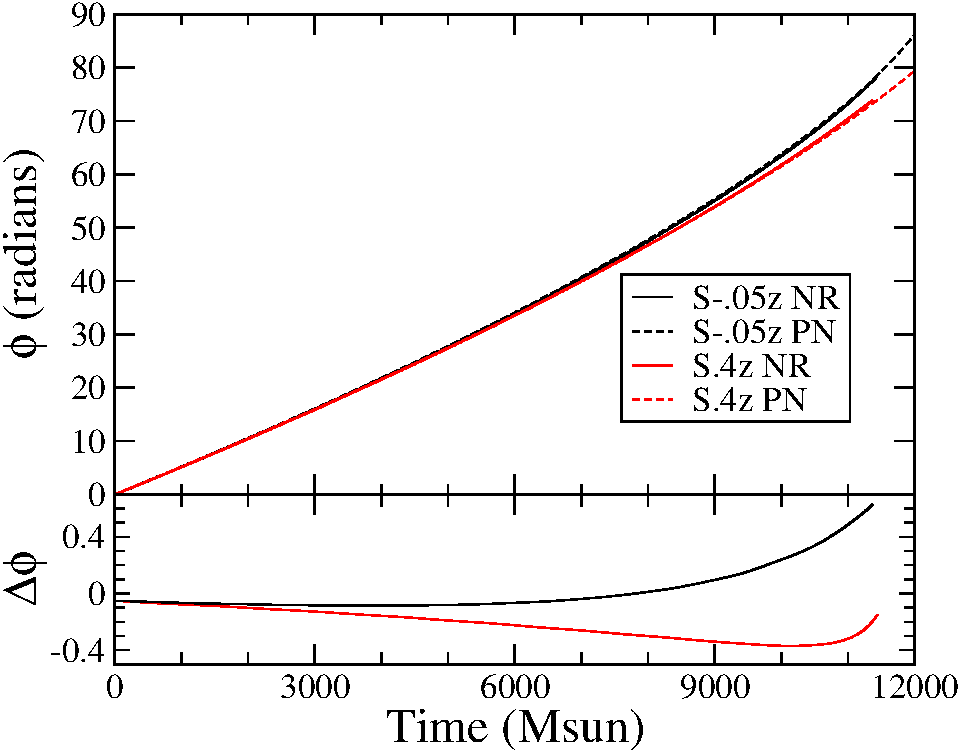
\includegraphics[width=0.95\columnwidth]{Hangup}
\caption{ {\label{fig:Hangup}} Accumulated orbital phase as a funciton
  of time for our anti-aligned, S-.05z, and aligned, S.4z,
  runs. The dashed lines are PN simulations using the same
  binary parameters. Qualitatively, there is excellent agreement with
  the numerical data. The lower panel shows the difference
    $\Delta\phi(t)=\phi_{rm NR}(t)-\phi_{\rm PN}(t)$. \red{Re-do analysis with proper matching procedure.}}
\end{figure}
%%%%%%%%%%%%%%%%%%%%%%%%%%%%%%%%%%%%%%%%%%%%%%%%%%%%%%%%%%%%%%%%


% Finally, it is well-known that the inspiral of aligned-spin binaries
% will proceed slower than anti-aligned-spin binaries, due to the
% orbital hang-up effect. We find clear evidence of this effect in
% comparing these two simulations. 

Finally, we compute the orbital phase 
\begin{equation}
\phi(t) = \int_0^t \Omega(t')\, dt',
\end{equation}
%and compare it to the post-Newtonian TaylorT4 model. 
%In figure~\ref{fig:Hangup} we plot
%the number of orbits as a function of time for both of these
%runs. The number of orbits is simply computed as
%\begin{equation}
%N(t) = \frac{1}{2\pi}\int_0^{t}\Omega(t)dt,
%\end{equation}
where the orbital frequency $\Omega(t)$ is given by
Eq.~(\ref{eq:Omega}).
The result is plotted in Fig.~\ref{fig:Hangup}, along with the
% is computed from the binary
% trajectory. We see that by the end of our simulations, the
% anti-aligned run is ahead by about half an orbit. In
% figure~\ref{fig:Hangup} we have also plotted the 
Post-Newtonian prediction for the same binary parameters (spins,
masses and initial orbital frequencies). We use the Taylor T4 model
\red{[REF]} at 3.5PN order expansion, with no tidal terms added, and
we have not used any additional matching methods. \red{[SERGEI, add
  details about PN model]} We find excellent qualitative agreement in
both cases, thereby giving additional evidence that our numerical
simulations are working as expected.

Figure~\ref{fig:AlignedGW} shows the gravitational waveforms for our
two aligned-spin simulations. We extract the waves on a sphere of
radius $R=627M_{\odot}$. 
%In practice, we directly extract the
%Newman-Penrose scalar $\Psi_4$ and compute $h$ by taking derivatives
%of $\Psi_4$ \red{[ERROR.  $\Psi_4$ is the time-derivative of $h$, so
%  you would have to integrate.  Check!]}. 
%By counting wave cycles, the
%orbital hangup effect can be seen here as well.

%%%%%%%%%%%%%%%%%%%%%%%%%%%%%%%%%%%%%%%%%%%%%%%%%%%%%%%%%%%%%%%%
\begin{figure}
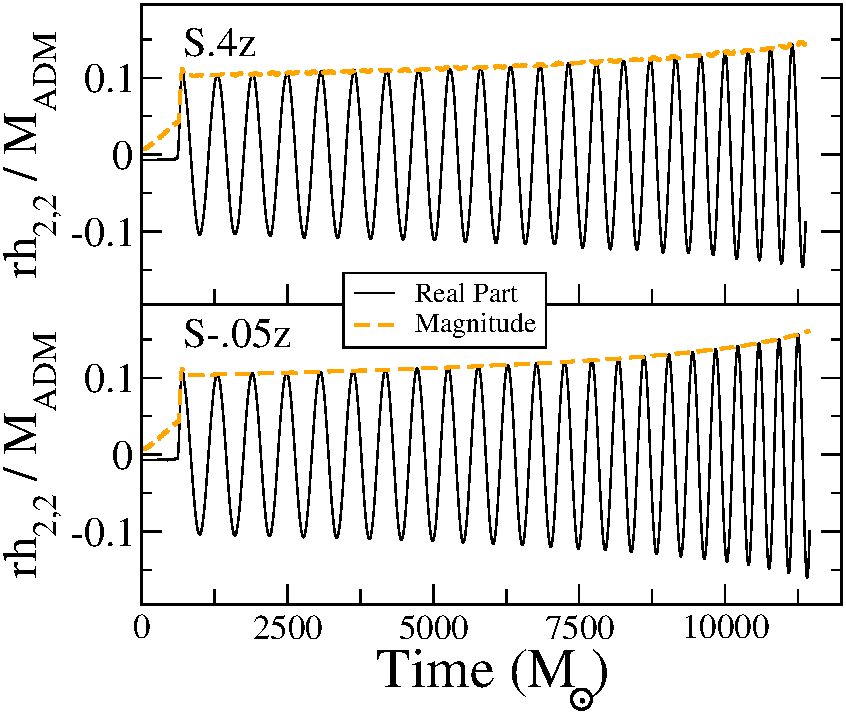
\includegraphics[width=0.95\columnwidth]{AlignedGW}
\caption { {\label{fig:AlignedGW}} The gravitational waveforms for our anti-aligned, S-.05z, and aligned, S.4z runs. The black curve represents the real part of the waveform, $\Re(h_{2,2})$ while the orange curve represents the magnitude of the waveform.}
\end{figure}
%%%%%%%%%%%%%%%%%%%%%%%%%%%%%%%%%%%%%%%%%%%%%%%%%%%%%%%%%%%%%%%%

%\item It is also important to show that the spins we measure during
%our evolutions converge in some sense with resolution. In
%figure~\ref{fig:ChiVTDifferentRes} we plot the spin measured during
%the evolution for three different resolutions. This is done for the
%S0.4z run, for the Ecc3 level of eccentriccity reduction. It is clear
%that all three resolutions seem to agree well, in the sense that the
%differences between resolutions are smaller than other sources of
%error. We also see that Lev2 is very close to Lev1. \red{It is
%unclear at this time what all the spikes in the spin are. They also
%don't seem to be present for other sized spheres. Very strange.}

%\begin{figure}
%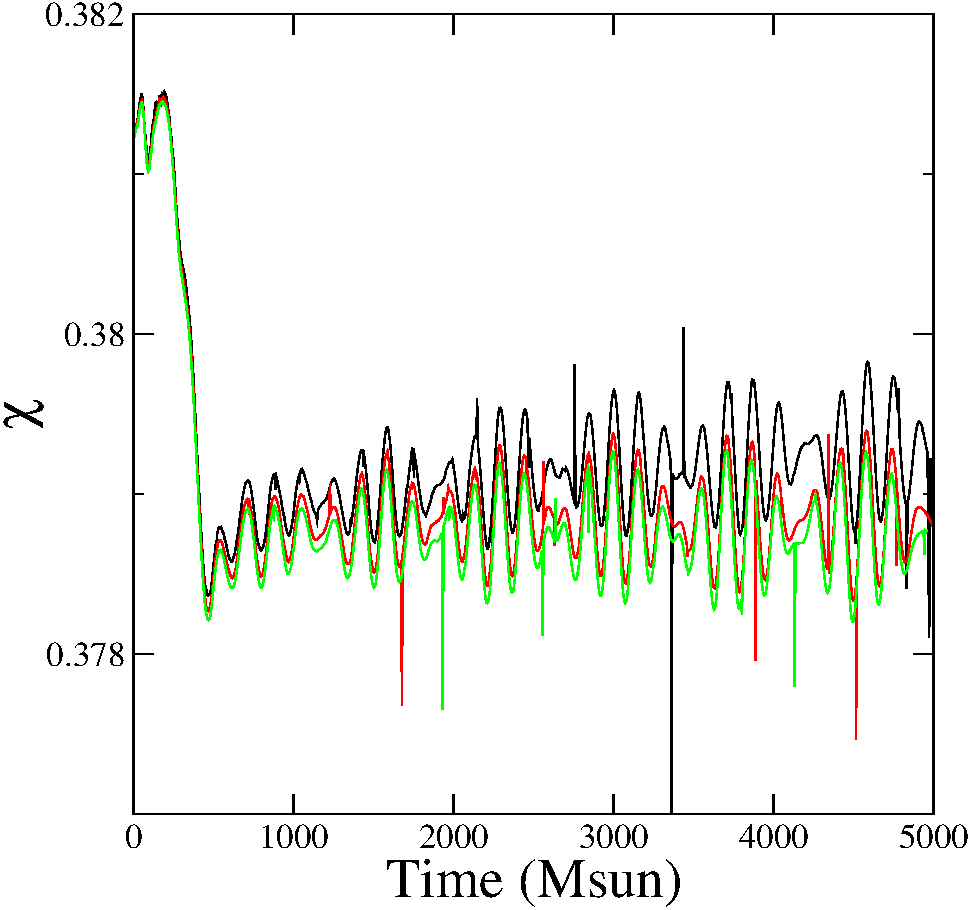
\includegraphics[width=0.95\columnwidth]{ChiVTDifferentRes} \caption{{\label{fig:ChiVTDifferentRes}}
%The spin measured during the evolution for three different
%resolutions.  \red{Downsample, include in Fig.~\ref{fig:ChiVTZoomed}}
%} \end{figure} \end{itemize} \begin{itemize} \item How do we compute
%NS spin during evolution \item Perhaps a plot showing the convergence
%of spin during evolution with the size of the spheres around the
%NS \item A plot like figure 14, showing both the difference between
%ID spin and evolution spin (typically $<1\%$) and how well the spin
%is maintained during the evolution. Perhaps a better case to show
%would be one with spins components in all three
%directions?  \end{itemize}

%\begin{figure}
%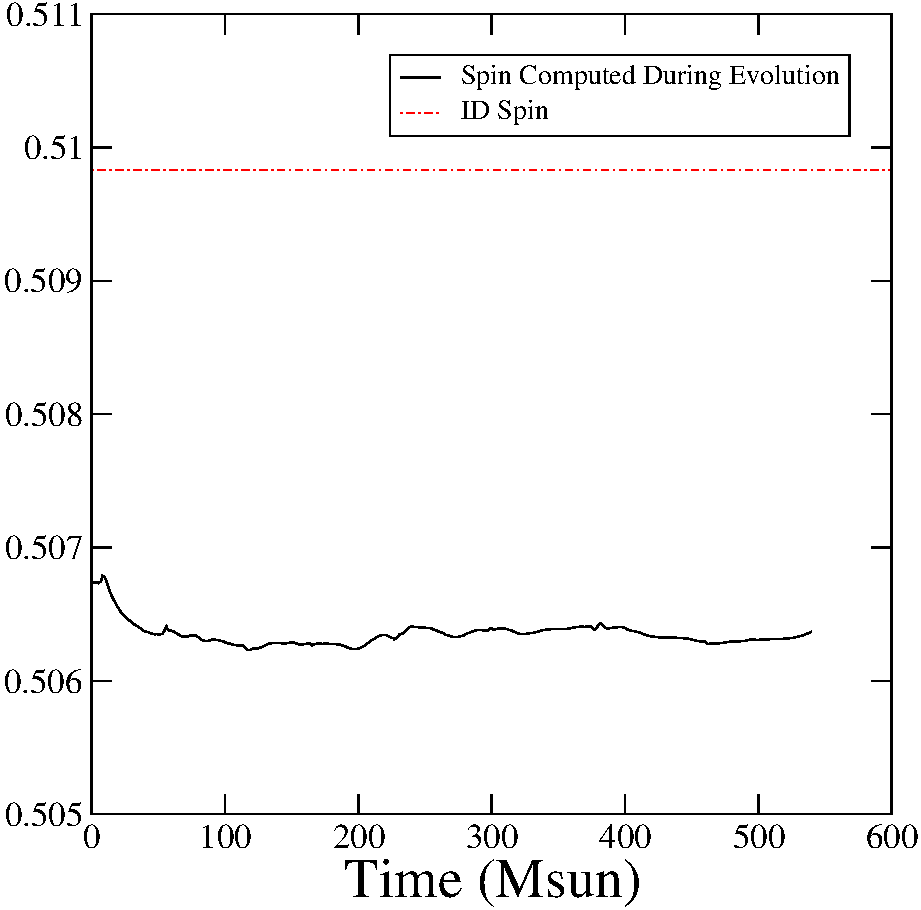
\includegraphics[width=0.95\columnwidth]{SpinDuringRun} \caption{The
%spin of a run with $\vec{\chi}\sim0.5\hat{z}$ as measured during the
%star's evolution} \end{figure}


%%%%%%%%%%%%%%%%%%%%%%%%%%%%%%%%%%%%%%%%%%%%%%%%%%%%%%%%%%%%%%%%
\begin{figure}
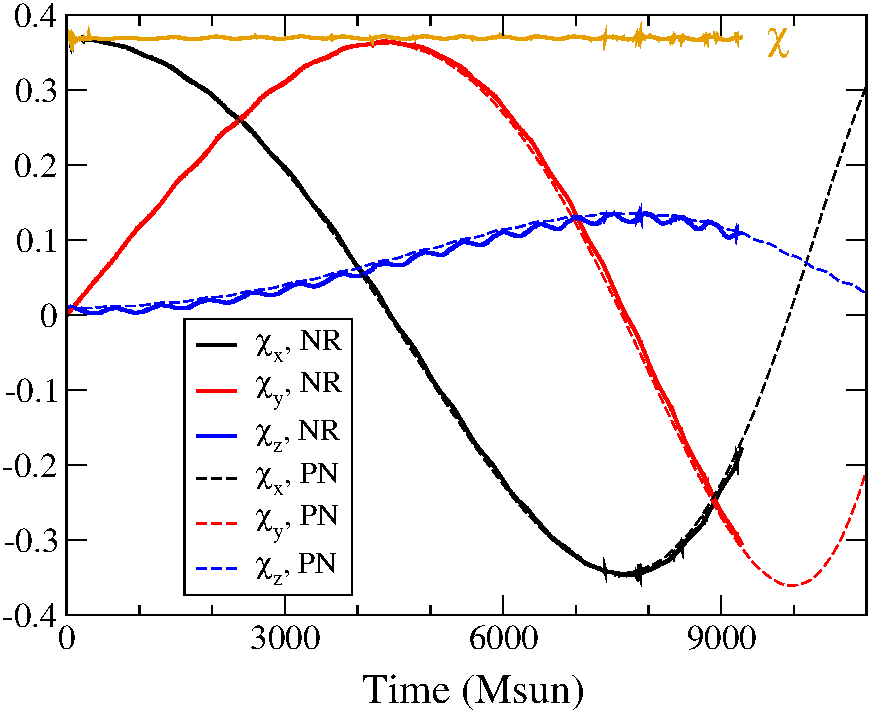
\includegraphics[width=0.95\columnwidth]{SpinComparison}
  \caption{\label{fig:FullPrec} Spin-components of one of the Neutron stars during the precessing simulation (thick, solid lines).  The thin dashed lines are a comparison to post-Newtonian theory.  The orange line denotes the spin magnitude $|\vec\chi(t)|$. \red{[Redo PN-NR comparison with changed normalization of $\chi$]} }
\end{figure}
%%%%%%%%%%%%%%%%%%%%%%%%%%%%%%%%%%%%%%%%%%%%%%%%%%%%%%%%%%%%%%%%

\subsection{Precession}


We now turn to the precessing simulation, S.4x.
Figure~\ref{fig:FullPrec} shows the components of the spin-vector
$\vec\chi$ of one of the Neutron stars, as a function of time.  The
quasi-local spin diagnostic returns a spin with nearly constant
magnitude, varying only by $\pm 0.002$ around its average value
$0.370$.  The spin components clearly precess, with the dominant
motion in the xy-plane (the initial orbital plane), with the
simulation completing about 2/3 of a precession cycle.  A z-component
of the NS spin also appears, indicating precession of the neutron star
spin out of the initial orbital plane.

%%%%%%%%%%%%%%%%%%%%%%%%%%%%%%%%%%%%%%%%%%%%%%%%%%%%%%%%%%%%%%%%
\begin{figure}
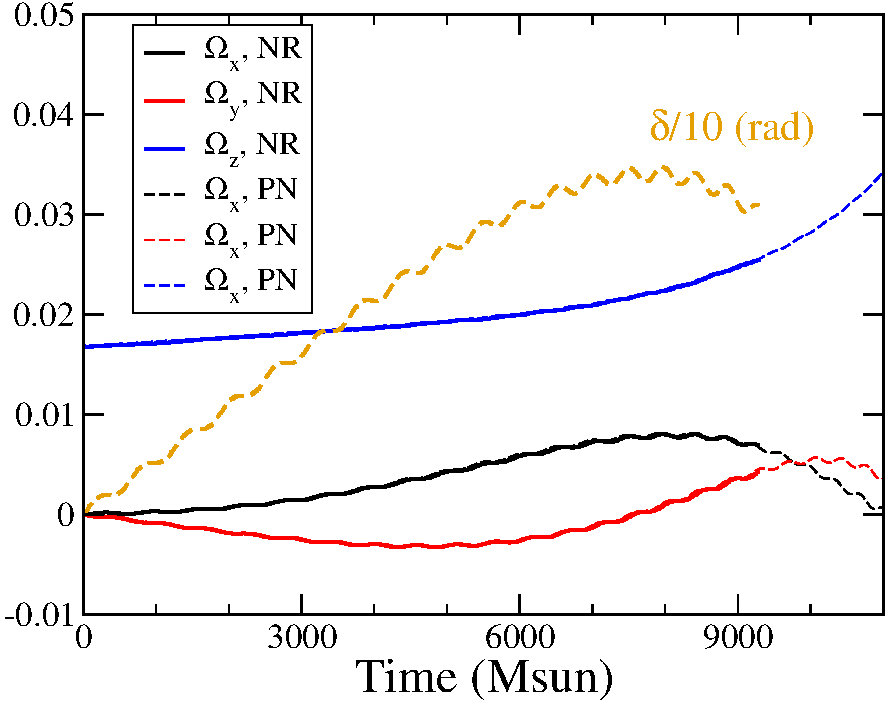
\includegraphics[width=0.95\columnwidth]{OmegaVectorComparison}
  \caption{\label{fig:OmegaVectorComparison} Components of the orbital frequency vector $\vec\Omega$.  Thick solid lines represent the precessing BNS simulation, and thin dashed lines a post-Newtonian comparison.  The inclination reaches $\delta=0.34\mbox{rad}\approx 20^\circ$ at $t=7600 M_\odot$.
  }
\end{figure}
%%%%%%%%%%%%%%%%%%%%%%%%%%%%%%%%%%%%%%%%%%%%%%%%%%%%%%%%%%%%%%%%


The dashed lines in Fig.~\ref{fig:FullPrec} represent a comparison to
the post-Newtonian precession equations. 

\red{[SERGEI:  give details]}

In this comparison, we simply initialize the PN equation with
spin-vectors and orbital frequency from the NS-NS initial data set,
and evolve independently.  \red{[SERGEI: correct as needed]} Even this
rather simple comparison yields astonishing agreement between the
solid (NR) and dashed (PN) curves in Fig.~\ref{fig:FullPrec}.  The NS
spins indeed precess as expected, thus confirming both the quality of
quasi-local spin measures, as well as the performance of the PN
equations.

The precession of the orbital angular frequency is shown in
Fig.~\ref{fig:OmegaVectorComparison}.  We find substantial precession
away from the initial direction of the orbital frequency
$\vec\Omega_0\propto \hat z$, with the angle $\delta$ between
$\vec\Omega(t)$ and the z-axis reaching $20^\circ$.  Once again, the
simple post-Newtonian model reproduces all features successfully.  
\red{[SERGEI:  more description here?]}

\begin{figure}
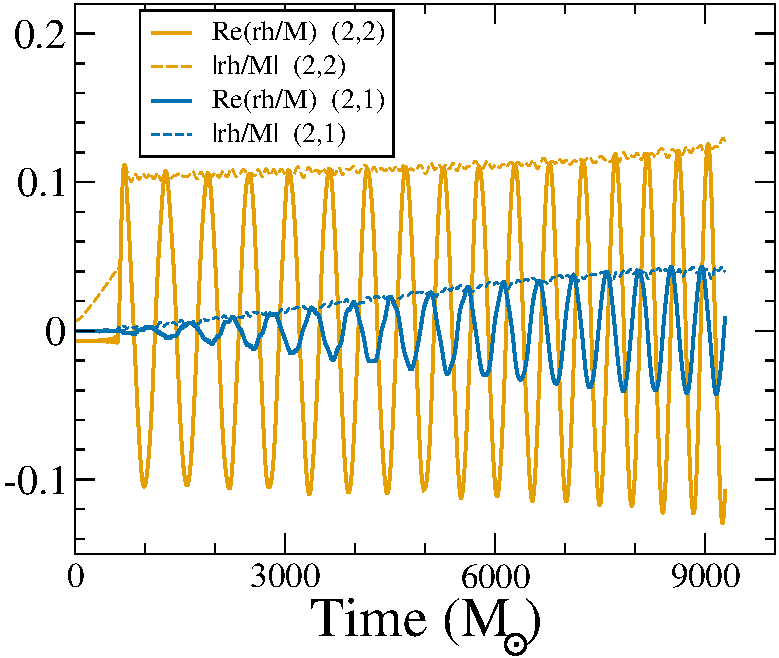
\includegraphics[width=0.9\columnwidth]{PrecGW}
\caption{\label{fig:PrecGW} Gravitational waveforms of our precessing
  run.  Shown are the $(l,m)=(2,2)$ and $(2,1)$ modes, as extracted in
  a spherical harmonic decomposition aligned with the z-axis.  The
  emergence of the (2,1) mode indicates precession of the orbital
  plane away from the xy-plane.}
\end{figure}


Finally, Fig.~\ref{fig:PrecGW} shows the (2,2) and the (2,1) spherical
harmonic modes of the gravitational wave-strain extracted at an
extraction surface of radius $R=647M_\odot$.  The
(l,m)=(2,1) mode would be identically zero for an equal-mass aligned
spin binary with orbital frequency parallel to the z-axis, so the
emergence of this mode once again indicates precession in this binary.

%\red{Obviously everything in this section is preliminary!}. \red{It
%  should eventually have a longer run, another spin configuration and
%  perhaps some comparison between NR results and PN predictions.}
%\begin{itemize}
%\item Our precessing run of interest begins with equal-mass NS with
%  equal spins, $\vec{\chi} = 0.37505\hat{x}$. From Kidder (1995), the
%  spin of the first star will evolve according to
%\begin{equation}
%\dot{\vec{S}}_1 =
%\frac{1}{r^3}\left(\left(\vec{L}_N\times\vec{S}_1\right)\left(2+\frac{3m_2}{2m_1}\right)-\vec{S}_2\times\vec{S}_1+3\left(\hat{n}\cdot\vec{S}_2\right)\hat{n}\times\vec{S}_1\right)
%\end{equation}
%Assuming that we can well approximate that the mass of the stars are
%constant, their orbital separation is constant, the orientation of the
%orbital plane is constant, and that $\vec{\chi}=0.37505\hat{x}$ can be
%taken as constant up to a small perturbation in the y direction, we
%find that the y component of the dimensionless spin of the first star
%will evolve according to
%\begin{equation}
%\dot{\vec{\chi}}_y = \frac{7M\omega\chi}{8r}
%\end{equation}
%In our code units we have $M=3.28$, $\omega=0.00510429$, $r=47.2$,
%$\chi=0.37505$, and so
%\begin{equation}
%\dot{\vec{\chi}}_y = 1.16 \times 10^{-4}
%\end{equation}
%In figure ~\ref{fig:ChiYVT} we plot $\vec{\chi}_y$ for this run (Ecc2)
%and the best fit line to the data. The best fit line forced through 0
%has a slope of $1.13\times 10^{-4}$, which is very close to the
%predicted value, and a good fit to the data, even though we clearly
%get into a regime where our assumptions start to break down.

%\begin{figure}
%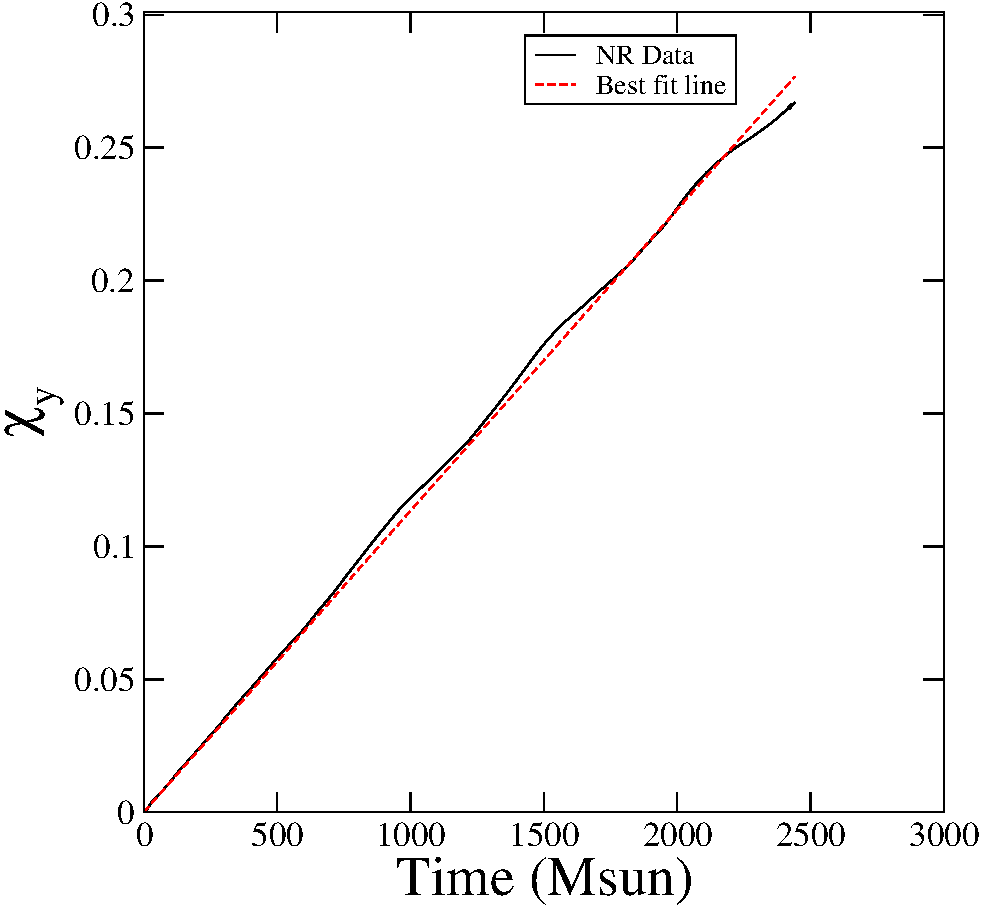
\includegraphics[width=0.95\columnwidth]{ChiYVT}
%\caption{{\label{fig:ChiYVT}} The time-evolution of the y-component of
%  the dimensionless spin for our precessing run. The red line is the
%  best fit line forced through 0 to the data, and its slope of
%  $1.13\times10^{-4}$ is in good agreement with the PN prediction
%  \red{[Great that precession works so well.  Work with Sergei toward
%      more accessible/intutive plots]}}
%\end{figure}

%\item A similar argument can be used to show that the x-component of
%  the spin will evolve according to:

%\begin{equation}
%\dot{\vec{\chi}}_x = \frac{7M\omega\chi_y}{8r}
%\end{equation}

%Using our approximation for $\chi_y$ from above, and integrating this,
%we arrive at the expression

%\begin{equation}
%\vec{\chi_x} = \chi_x(0) - 1.80\times10^{-8}t^2
%\end{equation}

%In figure~\ref{fig:ChiXVT} we plot the x-component of the
%dimensionless spin, and the best fit curve of the form $\chi = \chi_0
%- At^2$. The best fit value for $A$ is $1.89\times 10^{-8}$ - quite
%close to our predicted value.

%\begin{figure}
%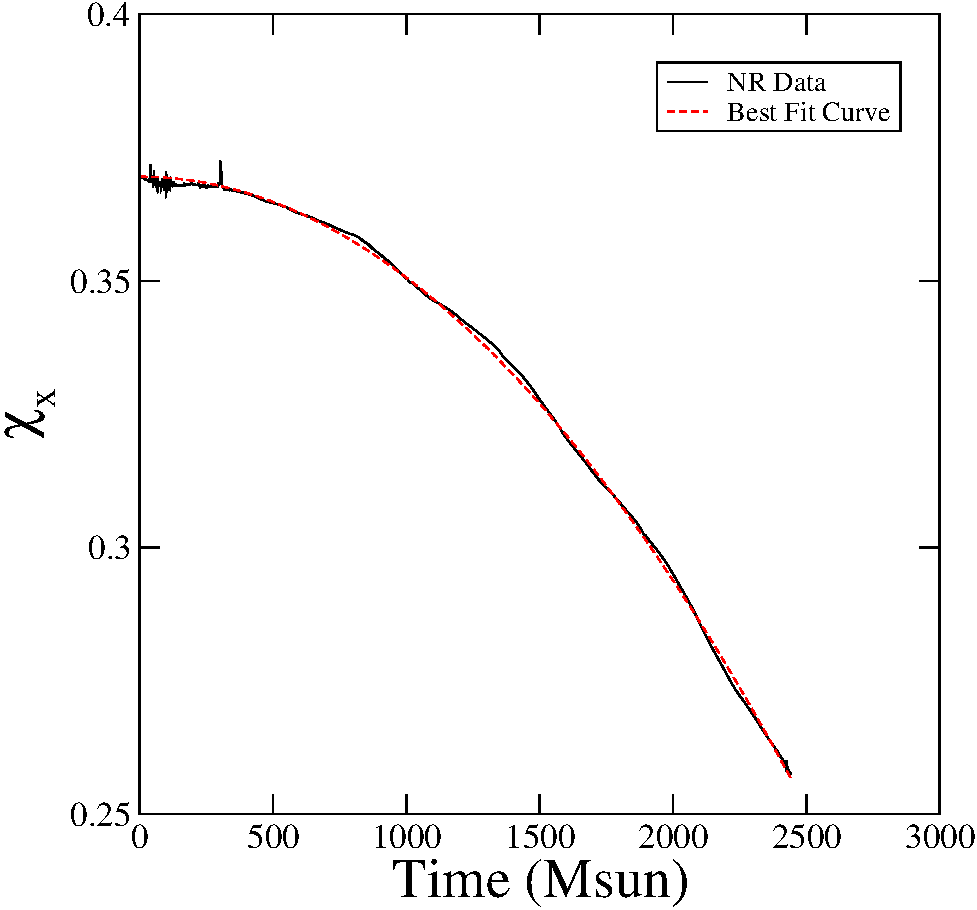
\includegraphics[width=0.95\columnwidth]{ChiXVT}
%\caption{{\label{fig:ChiXVT}} The time-evolution of the x-component of
%  the dimensionless spin for our precessing run. The red line is the
%  best fit line of the form $\chi = \chi_0 - At^2$, which agrees well
%  with the data, as well as the value predicted from PN.}
%\end{figure}

%\item \green{Really $\chi_x$ and $\chi_y$ should be a cosine and
%  sine. Could re-write them as such!}

%\item \green{Can we analyze the z-component of the spin?}

%\item We can also use this equation to predict the evolution of the
%z-spin for this binary. In this case, the evolution equation is

%\begin{equation} \dot{\chi}_z = \frac{7M}{8r}\left(-\omega_y\chi_x +
%\omega_x\chi_y\right) + \frac{3}{8r^3}\chi_x\chi_y \end{equation}
%Using our approximations above, this works out to \begin{equation}
%\dot{\chi}_z = -2.52\omega_y + 1.21\times10^{-9}\omega_yt^2 +
%7.78\omega_xt + \\1.55\times10^{-10}t^2 -
%7.45\times10^{-18}t^3 \end{equation}


%\item \green{To do: Some kind of more sophisticated PN/NR matching!
%  For the orbit as well!}




%\end{itemize}



%In figure 15 we plot $\vec{\chi}_y$ and the best fit line to the
%data. The slope of that line is $2.43 \times 10^{-5}$ - very close to
%the predicted value.  \begin{figure}
%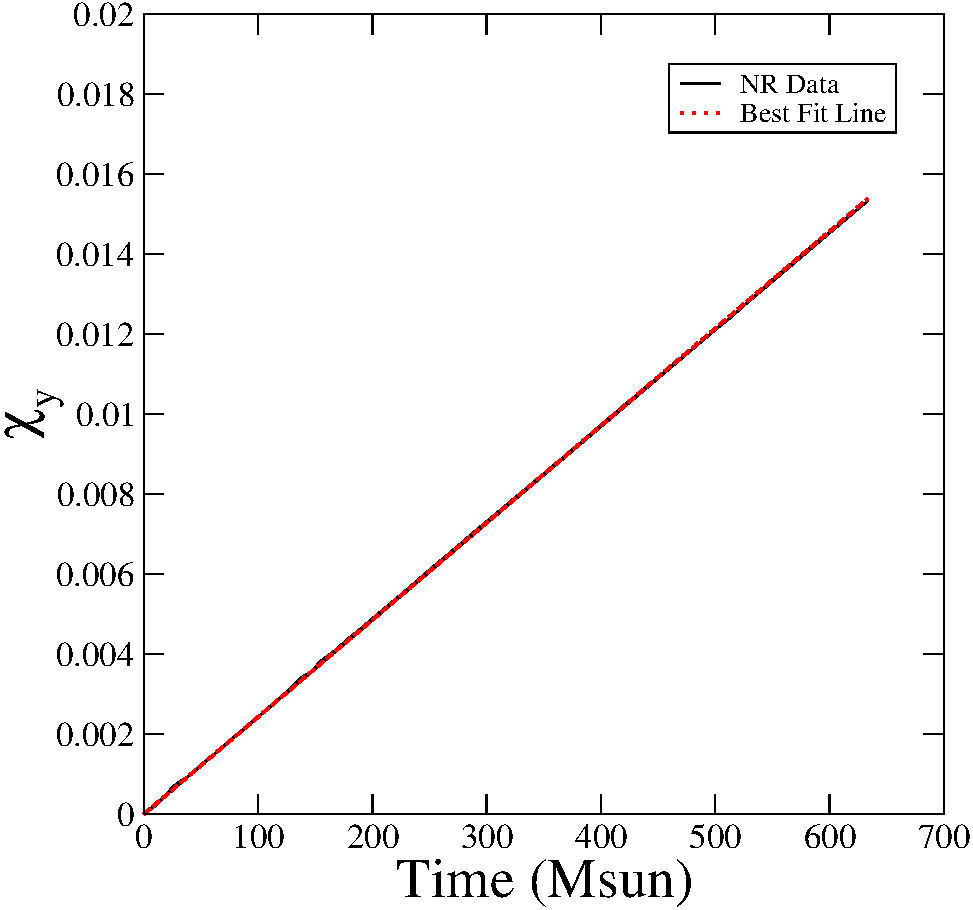
\includegraphics[width=0.95\columnwidth]{Precession} \caption{The y
%component of NS dimensionless spin for a precessing run starting wtih
%$\vec{\chi}=0.3\hat{x}$} \end{figure}


%%%%%%%%%%%%%%%%%%%%%%%%%%%%%%%%%%%%%%%%%%%%%%%%%%%%%%%%%%%%%%%%
\subsection{Stellar Oscillations}
\label{sec:QNModes}
%%%%%%%%%%%%%%%%%%%%%%%%%%%%%%%%%%%%%%%%%%%%%%%%%%%%%%%%%%%%%%%%

\begin{figure}
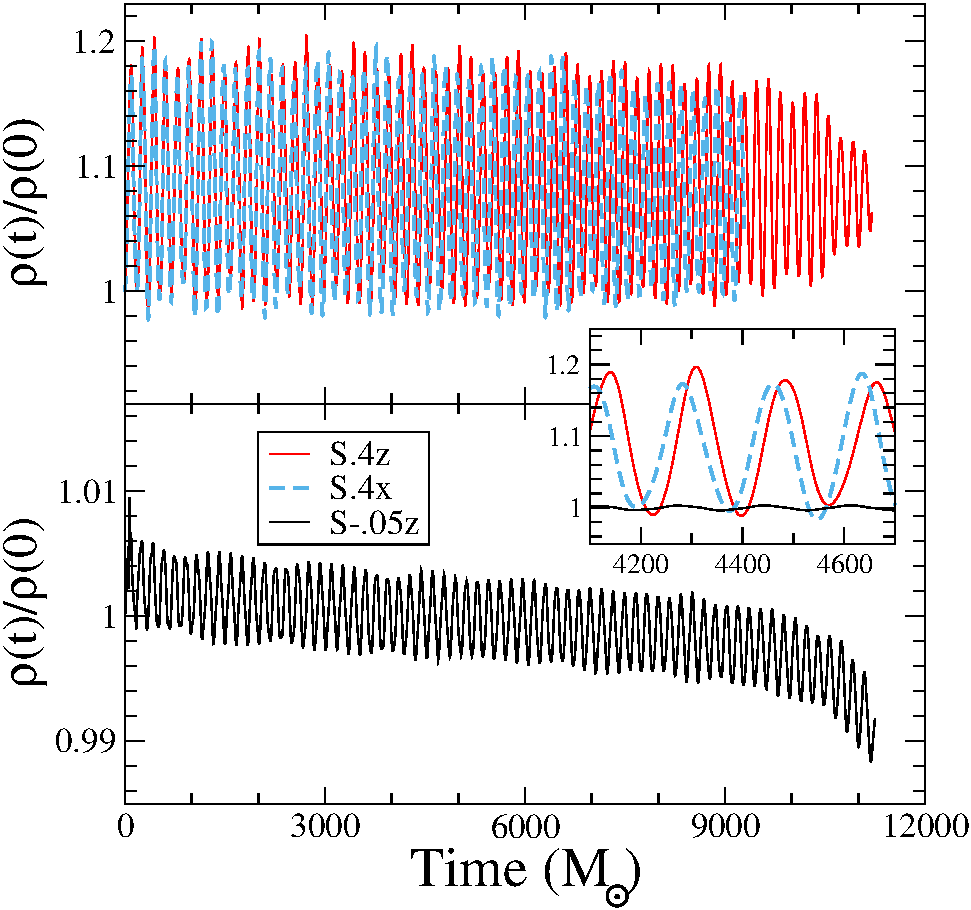
\includegraphics[width=0.95\columnwidth]{RhoMax}
\caption{\label{fig:RhoMax} The maximum density $\rho(t)$ in each of
  our runs, normalized by the initial maximum density $\rho(0)$.  The
  inset shows an enlargement of all three runs, illustrating that the
  oscillations are more pronounced in the high-spin simulations. }
\end{figure}

The rotating neutron stars constructed here show oscillations in the
central density, as plotted in Fig.~\ref{fig:RhoMax}.  In the low spin
run, the density oscillations have a peak-to-peak amplitude of about
0.6\%, whereas in the high-spin runs (S.4z and S.4x), the density
oscillations reach a peak-to-peak amplitude of 20\%.  The two
high-spin simulations show oscillations of nearly the same amplitude
and frequency, therefore oscillating nearly in phase throughout the
entire inspiral.  The the oscillation-period is about
$177 M_{\odot} \sim 0.87\rm{ms}$, i.e. giving a frequency of
$1.15kHz$.  It remains constant throughout the inspiral.  The low-spin
run S-0.5z exhibits a slightly smaller oscillation period of about
$P\approx 170M_{\odot}\approx 0.84\rm{ms}$, i.e. a frequency of
$\approx 1.19{\rm kHz}$.  

% \red{[Nick, please check conversion into SI  units]}
% \nick{
% \begin{eqnarray}
% \frac{P~G}{c^3} &=& \frac{170M_{\odot}~G}{c^3} \nonumber \\
% &=& \frac{\left(170\right)\left(2\times10^{30}\right)\left(6.7\times10^{-11}\right)}{\left(3\times10^{8}\right)^3} \nonumber \\
% &=& 0.0008437 \sim 0.84{\rm ms} \nonumber
% \end{eqnarray}
% }

%%%%%%%%%%%%%%%%%%%%%%%%%%%%%%%%%%%%%%%%%%%%%%%%%%%%%%%%%%%%%%%%
\begin{figure}
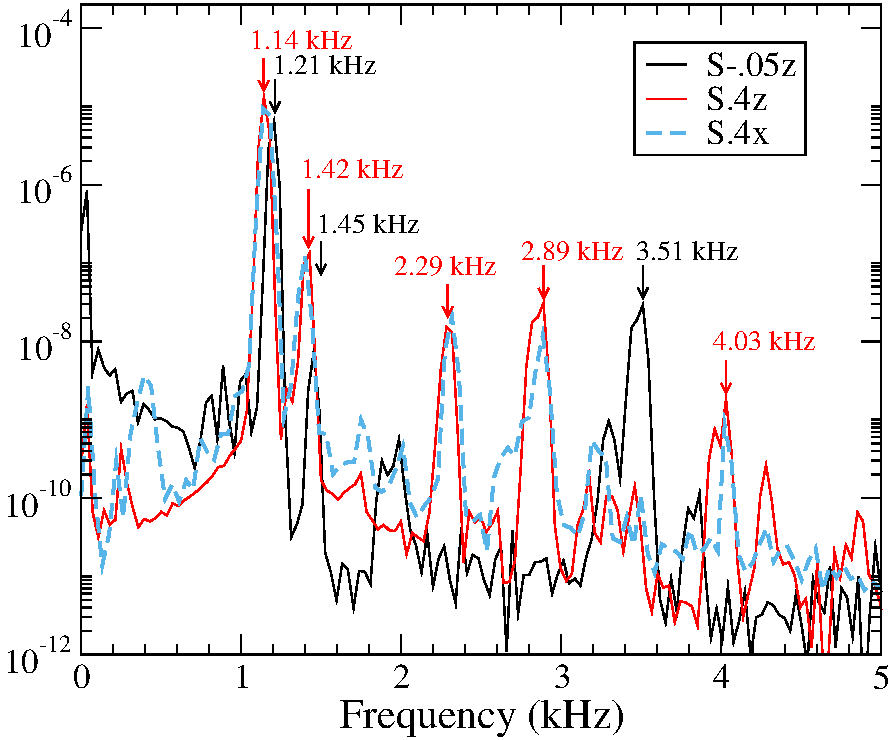
\includegraphics[width=0.95\columnwidth]{Density_FFT}
\caption{\label{fig:Density_FFT} The Fourier transforms of the central
  density in all three of our runs. Labelled are the peak frequencies
  for the quasi-radial F mode and the $l=2$, $^2f$ mode.}
\end{figure}
%%%%%%%%%%%%%%%%%%%%%%%%%%%%%%%%%%%%%%%%%%%%%%%%%%%%%%%%%%%%%%%%

To investigate the spectrum of the density oscillations, we perform a
Fourier-transform on $\rho(t)$.  The result is shown in
Fig.~\ref{fig:Density_FFT}.  The Fourier-transform confirms the
dominant frequencies just stated, and reveals several more frequency
components ranging up to 4kHz.  The high spin evolutions S.4z and
S.4x exhibit identical freqencies for all five discernible peaks.  In
contrast, the low-spin evolution S-.05z shows different frequencies.  

We interpret these features as a collection of excited quasi-normal
modes in each Neutron star.  The modes are excited because the initial
data is not precisely in equilibrium.  For the two high-spin cases the
Neutron stars have similar spin, and therefore the same quasi-normal
modes, whereas in the low-spin model, the quasi-normal mode
frequencies differ due to the different magnitude of the spin.

To strengthen our interpretation, we consider the series of rotating,
relativistic, $\Gamma=2$ polytropes computed by Dimmelmeier et
al~\cite{Dimmelmeier:2005zk}. 
%
%For a
%they computed the frequencies of the $l=0$ F mode, the $l=2$
%axisymmetric quadrupolar $^2f$ mode, and their overtones.  
%
Ref.~\cite{Dimmelmeier:2005zk}'s model ``AU3'' has a central density of
$1.074 \times 10^{-3} M_{\odot}^{-2}$ and its rotation is
quantified through the ratio of polar to equatorial radius,
$r_p/r_e = 0.780$.
%rough analogy with their results, we compare our highly-spinning
%models to their ``AU3'' model. As per their table 1, this run has a
%central energy density of $1.074 \times 10^{-3}$, and as a measure of
%rotational speed, they have $r_p/r_e = 0.780$.  
Meanwhile, our high-spin runs have a central density of
$1.02 \times 10^{-3} M_{\odot}^{-2}$ (measured as time-average of the data shown in
Fig.~\ref{fig:RhoMax}) and from our initial data, we find
$r_p/r_e \sim 0.8$. Given the similarity in these
values, we expect Ref.~\cite{Dimmelmeier:2005zk}'s ``AU3'' to approximate our high-spin
stars S.4x, S.4z.
Ref.~\cite{Dimmelmeier:2005zk} reports a frequency of
$f_F=1.283\rm{kHz}$ for the spherically symmetric ($\ell=0$) F-mode,
and a frequency $f_{2f}=1.537\rm{kHz}$ for the axisymmetric $\ell=2$
mode $^2f$.  These frequencies compare favourably with the two dominant
frequencies in Fig.~\ref{fig:Density_FFT}, $1.14\rm{kHz}$ and
$1.42\rm{kHz}$.
%
%Their model predicts
%$F=1.283\rm{kHz}$ and $^2f=1.537\rm{kHz}$. Meanwhile, the
%corresponding frequencies we identify are $F=1.14\rm{kHz}$ and
%$^2f=1.4\rm{kHz}$. 
Presumably, the small differences in these frequencies can be
accounted for by the slight differences in stellar mass, radius, and
rotation.  Moreover, tidal interactions and orbital motion could
factor in, as well. In our figure~\ref{fig:Density_FFT} we also see
several other peaks at higher frequencies, which are reminiscent of
the overtones and mode couplings in figure 10 of
\cite{Dimmelmeier:2005zk}. If we identify our peak at
  $f_{H1}=4.03\rm{kHz}$ with the $H_1$ mode, then (in analogy to
  \cite{Dimmelmeier:2005zk} Fig.~10), 
  $f_{H1}-f_{F}=(4.03-1.14)\rm{kHz}=2.89\rm{kHz}$, and
  $2f_{F}=2.28\rm{kHz}$, two frequencies that are indeed present in
  our simulations.
Although we find clear indications of axisymmetric $\ell=2$-modes,
we note that their power in smaller by two orders of magnitude,
compared to the spherically symmetric, dominant $F$ mode. 

Turning to the low-spin run S.05z, we note that if, to first order,
these frequencies scale like $f\sim\sqrt{\rho}$ (on dimensional grounds), then we expect to see
$F=1.22\rm{kHz}$ and $^2f=1.49\rm{kHz}$. This is very close to what is
seen.


The density oscillations discussed in this section are reflected in
analogous oscillations in various other diagnostic quantities, for
instance, the orbital frequency, Fig.~\ref{fig:OmegaDotComparison} and
the quasi-local spin as shown in Fig.~\ref{fig:ChiVTDifferentRes2}.
The domiant frequencies $1.14\rm{kHz}$ and $1.42\rm{kHz}$ can be
robustly identified throughout our data analysis. In
figure~\ref{fig:ManyQuantities} we plot the Fourier transform of the
density, the $(2,0)$ and $(2,2)$ gravitational wave strains, the
orbital angular velocity time derivative $d\Omega/dt$ and the
measured spin $\chi$ for the S.4z run. All show peaks in power at
these two frequencies, $F\sim1.14\rm{kHz}$ and $^2f\sim1.4\rm{kHz}$.


\begin{figure}
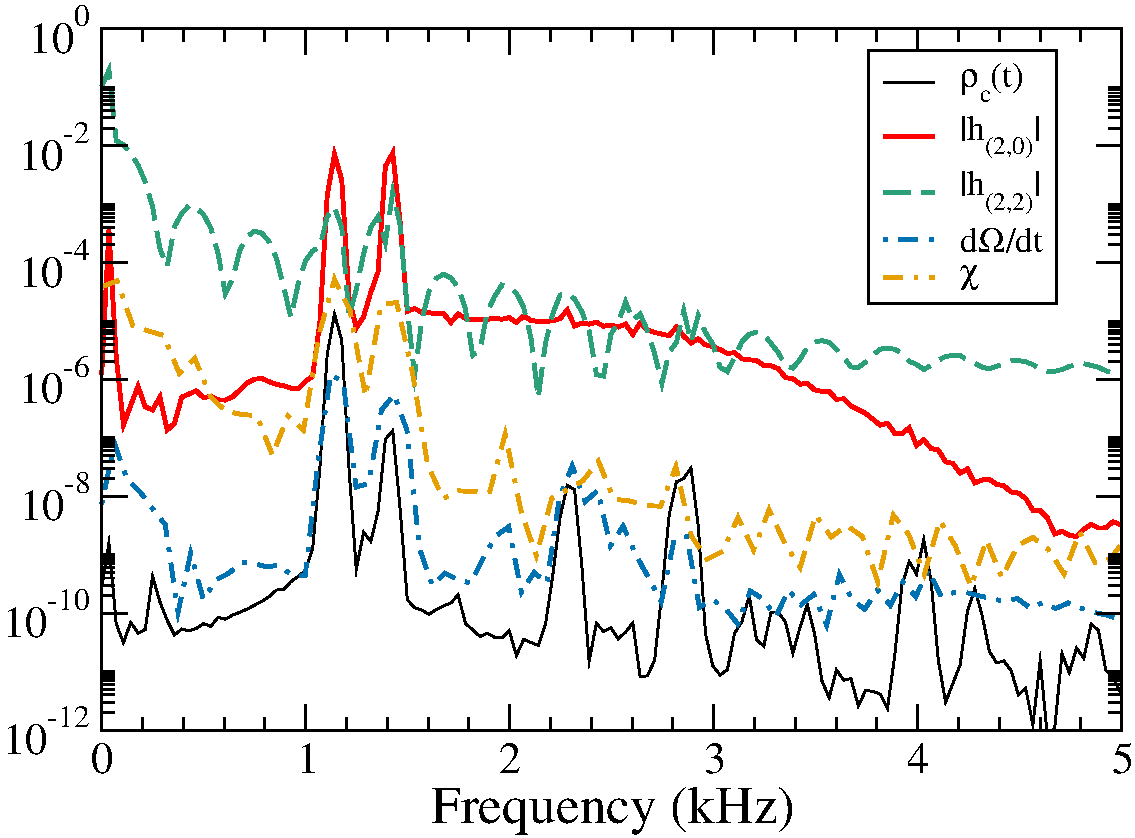
\includegraphics[width=0.95\columnwidth]{ManyQuantities}
\caption{\label{fig:ManyQuantities} Fourier transforms of the central
  density $\rho_c(t)$, two modes of the gravitational wave strain
  $(h_{2,2}$ and $h_{2,0}$), $\dot{\Omega}$ and $\chi$ for the S.4z
  run.  All quantities show excess power at $1.14\rm{kHz}$ and
  $1.4\rm{kHz}$, corresponding to the frequencies of excited neutron
  star quasi-normal modes.}
\end{figure}


\red{[Note other places in the literature where such oscillations are
  observed.  Note how large/small they are in irrotational NSNS
  systems]}

% It is also interesting that both cases start near in a
% minium in density. Fig.~\ref{fig:RhoMax} also shows that these
% oscillations are present in the anti-aligned case as well, although
% the oscillations are significantly smaller in amplitude - about
% $0.4\%$ from mean-value to peak. 

We believe  that the  stellar  modes are  excited because  the
  initial  data  are  not  in  perfect  equilibrium.   We  expect  the
  quasi-equilibrium  approximations   that  enter  the   initial  data
  formalism to become less valid  at higher spins, consistent with our
  observation that the high spin models exhibit stronger oscillations.
  This  interpretation is  strengthened by  additional simulations  of
  Neutron stars at larger separation. Increasing   the  intial
  separation  by  a  factor  1.5,  while  keeping  the  same  rotation
  parameter  $\omega$  as  in  the  S.4z-case,  we  find  quasi-normal
  oscillations   of  similar   amplitude  than   in  S.4z.    If  the
  oscillations were  caused by  the neglect  of tidal  deformation, we
  would expect the amplitude to drop with the 3rd power of separation,
  inconsistent with our results.


Finally, we point out that the radial rotation profile,
  cf. Eq.~(\ref{eq:UniformRotation}) influences the amplitude of the
  induced quasi-normal oscillations.  If the initial data is
  constructed with the rotation profile
  Eq.~(\ref{eq:ConformalUniformRotation}), instead of
  equation~\ref{eq:ConformalUniformRotation}, then the amplitude of
  the density oscillations for high spin doubles. This further
  supports our conjecture that the origin of this mode comes from
  non-equilibrium initial data.

% Complications from this mode have shown up throughout our paper. We
% believe that the large noise apparent in $\dot{Omega}(t)$ in our
% eccentriccity reduction analysis is due to these density
% oscillations. That noise has a periodic component which is similar
% to that of the density oscillations. Another place it shows up is in
% the gravitational waveforms. Although it is somewhat hard to see in
% figure~\ref{fig:AlignedGW}, the gravitational wave signal from the
% S0.4z run is more ``messy'' than that of the S-0.05z run. This is
% because its magnitude has a small periodic component which has a
% similar period to the density oscillations. This is true of the
% S0.4x gravitational waveform shown in figure~\ref{fig:PrecGW} as
% well.





%\begin{itemize}
%\item Describe what's been tried and outcome
%\item Shear
%\item A plot of normalized density vs. time for several different
%  spins could be interesting.
%\end{itemize}

%\end{itemize}

\section{Discussion}
\label{sec:Discussion}

% Using Tichy's method, we have constructed initial data with the SpEC
% code for BNS with dimensionless spins of up to 0.45.

% We present detailed convergence tests of these initial data, showing
% spectral and iterative convergece.

In this paper we implement Tichy's method~\cite{Tichy:2012rp} to
construct binary neutron star initial data with arbitrary rotation
rates.  We demonstrate that our implementation is exponentially
convergent, as expected for the employed spectral methods.

% We introduce a method to directly and robustly measure the NS spin
% using the method of quasi-local Killing vectors.

We measure the spin of the resulting neutron stars using the
quasi-local angular momentum
formalism~\cite{BrownYork1993,Cook2007,Lovelace2008,OwenThesis}.  The
resulting angular momentum is found to be nearly independent on the
precise choice of extraction sphere, cf. Fig.~\ref{fig:ChiVR}, and
provides a means to define the quasi-local angular momentum of each
neutron star to about 1\%, both in the initial data and during the
evolution, cf. Fig.~\ref{fig:ChiVTZoomed}.  We are able to construct
binary neutron star initial data with dimensionless angular momentum
of each star as large as $\chi=S/M^2\sim 0.44$, both for the case of
aligned spins, and also for a precessing binary where the initial
neutron star spins are tangential to the initial orbital plane.


% We present low-eccentriccity $\sim 10$ orbit evolutions of three
% systems - Low spin anti-aligned, high spin aligned and high spin
% precessing.

When evolving the initial data sets, the dimensionless spin measured
in the initial data drops by about 0.004, and then remains constant
through the 10 inspiral orbits for which we evolved the neutron star
binaries.  During these evolutions, we also demonstrated iterative
eccentricity removal: By analyzing the orbital frequency $\Omega(t)$
during the first few orbits, we can correct the initial data
parameters $\Omega_0$ and $\dot a_0$, and thus decrease the orbital
eccentricity from $e\approx 0.01$ to $e\lesssim 0.001$.

% We find good(?) matches with PN for orbital and spin dynamics
% (quantify)

For the precessing simulation S.4x, we find precession of the neutron
star spin directions.  The numerically established precession of the
spin axes and of the orbital angular momentum agrees well with
post-Newtonian predictions.

% We find an excited quasi-normal vibrational mode in our evolutions,
% which is especially visible in the highly spinning systems, giving
% rise to up to $\tilde 10\%$ density oscillations. This is believed
% to be due to imperfections in the initial data.

The rotating neutron stars constructed here exhibit clear signals of
exciting quasi-normal modes.  We are able to identify multiple modes
in the Fourier spectrum of the central density.  The amplitude of the
excited quasi-normal modes increases steeply with rotation rate of the
Neutron stars.  For S-.05z (spin magnitude $\chi=0.045$) the density
oscillations have peak-to-peak amplitude of 0.6\%, raising to 20\% for
the two runs with high spins (S.4x and S.4z).  

\begin{comment}
\begin{figure}
\includegraphics[width=0.95\columnwidth]{S_005z_Px}
\end{figure}
\begin{figure}
\includegraphics[width=0.95\columnwidth]{S_005z_Py}
\end{figure}
\begin{figure}
\includegraphics[width=0.95\columnwidth]{S_005z_Pz}
\end{figure}
\begin{figure}
\includegraphics[width=0.95\columnwidth]{S_04z_Px}
\end{figure}
\begin{figure}
\includegraphics[width=0.95\columnwidth]{S_04z_Py}
\end{figure}
\begin{figure}
\includegraphics[width=0.95\columnwidth]{S_04z_Pz}
\end{figure}
\begin{figure}
\includegraphics[width=0.95\columnwidth]{S_04x_Px}
\end{figure}
\begin{figure}
\includegraphics[width=0.95\columnwidth]{S_04x_Py}
\end{figure}
\begin{figure}
\includegraphics[width=0.95\columnwidth]{S_04x_Pz}
\end{figure}
\end{comment}


\begin{acknowledgments}
We thank \red{N.N. and N.N}.
Calculations were performed with the {\tt
  SpEC}-code~\cite{SpECwebsite}.  We gratefully acknowledge support
from NSERC of Canada, from the Canada Research Chairs Program, and
from the Canadian Institute for Advanced Research.  
\red{[ADD GRANTS]}
%We further
%gratefully acknowledge support from the Sherman Fairchild Foundation;
%from NSF Grants PHY-1306125 and AST-1333129 at Cornell; and from NSF
%Grants No. PHY-1440083 and AST-1333520 at Caltech.  
Calculations were performed at the GPC supercomputer at the SciNet HPC
Consortium~\cite{scinet}; SciNet is funded by: the Canada Foundation
for Innovation (CFI) under the auspices of Compute Canada; the
Government of Ontario; Ontario Research Fund (ORF) -- Research
Excellence; and the University of Toronto.  
\red{[other HPC systems?]}
%Further computations were
%performed on the Zwicky cluster at Caltech, which is supported by the
%Sherman Fairchild Foundation and by NSF award PHY-0960291; and on the
%NSF XSEDE network under grant TG-PHY990007N.%\\
\end{acknowledgments}


\bibliography{../References/References}

\end{document}

\clearpage

\appendix

\section{Rotation periods}
To compute the physical spin period of each star, we first set up an
equivalent system with no orbital velocity, so that all the motion
comes from the spin. We then compute the angular frequency as
\begin{equation}
\Omega = \frac{\rm{max}\{V\}}{R_{\rm{eq}}} = \frac{\rm{max}\{\sqrt{g_{ij}u^iu^j}\}}{R_{\rm{eq}}}
\end{equation}
These runs are summarized in table 1 below. The spin period is then
computed as $P=\frac{2\pi}{\Omega}$. %\todo[color=red]{Check! -NT}.

\begin{table}
\begin{tabular} {c | c | c}
Run Name & $\bf{\chi}$ & Spin Period(ms)  \\ \hline S-.05z & $-0.050176\hat{z}$ & $11.0\rm{ms}$
\\ S.4z & $0.380178\hat{z}$ & $1.7\rm{ms}$ \\ S.4x & $0.375052\hat{x}$ & $1.7\rm{ms}$ \\
\end{tabular}
\caption{\red{[Add caption]} \red{[Table moved here from the Initial-Data section.  Consider precise placement when polishing Evolution-Section]}
}
\end{table}



\section{Trajectories}
\begin{figure*}
\includegraphics[width=0.66\columnwidth]{S005zTraj}
\includegraphics[width=0.66\columnwidth]{S04zTraj}
\includegraphics[width=0.66\columnwidth]{S04xTraj}
\caption{Trajectories for the three evolutions, at lowest eccentricity.}
\end{figure*}


%\section{Ongoing Runs/Work}
%This section is not to be included in the paper. Just useful for me to
%keep track of what's ongoing.

%\begin{itemize}
%\item bla
%\end{itemize}

%\appendix
%\section{A calculation}
%Tichy's claim is that
%\begin{equation}
%\gamma^{\nu}_{i}\mathcal{L}_{\xi}\left(\nabla_{\nu}\phi\right)\approx0
%\end{equation}
%means that the time derivative of the irrotational piece of the fluid
%velocity vanishes in corotating coordinates. Let us further
%investigate this claim...
%\begin{eqnarray}
%\gamma^{\nu}_{i}\mathcal{L}_{\xi}\left(\nabla_{\nu}\phi\right)&\approx&0\\ \gam%ma^{\nu}_i\xi^{\mu}\nabla_{\mu}\nabla_{\nu}\phi
%+ \gamma^{\nu}_{i}\nabla_{\mu}\phi\nabla_{\nu}\xi^{\mu}&\approx& 0
%\end{eqnarray}
%If we take $\xi$ to be a Killing vector, then we can write
%\begin{equation}
%\gamma^{\nu}_i\xi^{\mu}\nabla_{\mu}\nabla_{\nu}\phi -
%\gamma^{\nu}_{i}\nabla_{\mu}\phi\nabla^{\mu}\xi^{\nu}\approx 0
%\end{equation}
%In corotating coordinates, $\xi$ is purely timelike, so we can write:
%\begin{equation}
%\xi^{\mu} = \left(\xi,0,0,0\right)
%\end{equation}.
%Then,
%\begin{eqnarray}
%\gamma^{\nu}_i\xi\nabla_{t}\nabla_{\nu}\phi -
%\gamma^{\nu}_{i}\nabla_{\mu}\phi\nabla^{\mu}\xi^{\nu}&\approx&
%0\\ \xi\nabla_{t}\nabla_{i}\phi -
%\nabla_{\mu}\phi\nabla^{\mu}\xi^{i}&\approx& 0
%\end{eqnarray}
%The second term vanishes because $\xi^i=0$, so we are left with
%\begin{equation}
%\nabla_t\nabla_i\phi \approx 0
%\end{equation}
%So in this sense the time derivative of the irrotational part of the
%fluid velocity is 0 in the corotating frame.

%\red{Still an open question: Is this the same as
%\begin{equation}
%\partial_t\nabla_i\phi \approx 0?
%\end{equation}. Does it matter?}

%\section{Another Calculation}
%Tichy's claim is that the equations
%\begin{eqnarray}
%\gamma^{\nu}_i\mathcal{L}_{\frac{\nabla\phi}{hu^0}}w_{\nu}&\approx&
%0\\ ^{\left(3\right)}\mathcal{L}_{\frac{w}{hu^0}}w_i &\approx& 0
%\end{eqnarray}
%describe the fact that the rotational piece of the fluid velocity is
%constant along the world line of the star center. Let us invesitage
%this claim. If we play fast and loose with the indices and dimensions,
%we can write something like
%\begin{eqnarray}
%\gamma^{\nu}_i\mathcal{L}_{\frac{\nabla\phi}{hu^0}}w_{\nu} +
%^{\left(3\right)}\mathcal{L}_{\frac{w}{hu^0}}w_i &\sim&
%\mathcal{L}_{\frac{\nabla_{\phi}+w}{hu^0}}w_{i}
%\\ &=&\mathcal{L}_{\frac{u}{u_0}}w_{i}
%\end{eqnarray}
%Which kind of agrees with the statement. \red{Still not sure how to
%  make this all work formally though.}

%\section{Code to compute QL spin}
%\green{The observer is:}
%\begin{verbatim}
%StrahlkorperPhysicalQuantities =( Surface = SurfB_One; Interpolator =
% CardinalInterpolator; SpatialCoordMapFromAHToMeasurementFrame =
% IDMap::SpatialCoordMap; Metric = g; ExtrinsicCurvature = K; InvMetric
% = Invg; Christoffel2ndKind = Christoffel2ndKind; Ricci = Ricci; Norm
% = CookWhiting; FindMinMaxRWithMinimizationAlgorithm = false;
% FindMinMaxRWithInterpolation = true;)
%\end{verbatim}
%\green{The surface SurfB\_One is computed by something like}
%\begin{verbatim}
%StarSurface = ( Output = SurfB_One; Lmax = 11; Mmax = 11; Symmetry =
% 0; TargetH = 1.000; Center = -37.5,0,0; Subdomain = StarOutA_One0;
% etc.)
%\end{verbatim}
%\green{The output might look something like (this is a spin-aligned
%  case):}
%\begin{verbatim}
%Sx / M^2 = -1.08...e-09 Sy / M^2 = 7.527...e-10 Sz / M^2 = 0.02553...
%  |S| / M^2 = 0.02553...  M = Christodolou Mass = 6.2562...  Mirr =
% Irreducible Mass = 6.2557...
%\end{verbatim}
%\green{I then compute the angular momentum of the Neutron star by
%  multiplying each of the first three components by the square of the
%  Christodolou mass. I then compute the dimensionless spin of the
%  Neutron star by dividing by the square of its ADM mass. Not entirely
%  sure if it should be this or the baryon mass. Also the code, right
%  now as far as I can tell, doesn't output the mass of each star
%  anywhere, so I am just using the value that I want the code to make
%  it (e.g. 1.4).}



%\newpage
%\section*{References}
%\bibliographystyle{unsrt} 



%%%%%%%%%%%%%%%%%%%%%%%%%%%%%%%%%%%%%%%%%%%%%%%%%%%%%%%%%%%%%%%%
\section{Equation of State}
%%%%%%%%%%%%%%%%%%%%%%%%%%%%%%%%%%%%%%%%%%%%%%%%%%%%%%%%%%%%%%%%

\red{[HARALD uncommented this section, to remind himself what it contained.  It would be good to keep some of the ID sets here, to demonstrate robustness of the initial-data code.  Especially the $\Gamma=3$ case is interesting.  However, I am not convinced we have taken into account correctly all scalings.  For instance, I believe that $\Gamma=2$ polytropes are mass-invariant.  Chaning $\kappa$ for $\Gamma=2$ merely moves along this mass-invariant curve.  If we were to scale all other parameters appropriately with $\kappa$, I would expect no change at all.]}

A final way to test the validity of the physics of our star, is to
check if $\chi$ responds as expected when the radius of the star is
changed (and everything else remains fixed). We do this by changing
$\kappa$ in our polytropic equation of state. From consideration of
hydrostatic equilibrium:
\begin{eqnarray}
\frac{GM^2}{R^4} &\sim& P \\ \frac{GM^2}{R^4} &\sim& \kappa\rho^2
\\ \frac{GM^2}{R^4} &\sim& \frac{\kappa M^2}{R^6}\\ R^2 &\sim&
\frac{\kappa}{G}
\end{eqnarray}
Now the dimensionless spin scales like
\begin{eqnarray}
\chi &\sim& \frac{f\omega R^2}{M} \\ \chi &\sim& \frac{f\omega
  \kappa}{GM}
\end{eqnarray}
Here $f$ is a dimensionless number relating moment of inertia to
angular momentum. It is typically $\sim 0.33$ for neutron stars
\red{[cite?]}. We thus predict a linear relationship between $\chi$
and $\kappa$ for $\Gamma=2$ neutron stars, as long as we are in a
regime where $f$ is roughly constant. In figure~\ref{fig:ChiVKappa} we
plot $\chi$ for a series of initial data sets with $\omega=0.01$,
$M=1.64M_{\odot}$, and $\kappa$ varying from 113.6 to 148.6. We find a
clear linear relation between the two, as expected.
\red{[Harald:  Aehm, not at all.  You predict $\chi\propto \kappa$, and you find $\chi=A+B\kappa$ for {\bf non-zero} $A$.  A fit $\chi=A\kappa$ is really bad.  A power-law fit $\chi=A\kappa^n$ gives $n\approx 2$, so not linear at all.]}


\begin{figure}
\includegraphics[width=0.95\columnwidth]{ChiVKappa}
\caption{{\label{fig:ChiVKappa}}$\chi$ as a function of the polytropic
  EOS parameter $\kappa$ for $\Gamma=2$ polytropes. The relation is
  linear, as expected ($R^2\sim 0.99985$).}
\end{figure}

A similar argument to that above tells us that for $\Gamma=3$
polytropes, the dimensionless spin scales like
\begin{equation}
\chi \sim \frac{f\omega \kappa^{2/5}}{M^{3/5}}
\end{equation}
In figure ~\ref{fig:ChiVKappaGamma3} we show a log-log plot of $\chi$
vs. $\kappa$ for a wide-range of $\Gamma=3$ polytropes, as well as the
best-fit power law to the data. The best fit has a slope of $0.47$,
somewhat close to the predicted value of $0.4$. \red{Why the
  discrepency? Is this important?  [HP: just state what it is, and
    point to the uncertainities in the estimate]}

\red{[Conclude section with: Robust ID code: Can handle various
    spin-magnitudes, and directions.  Also different EOS]}


\begin{figure}
\includegraphics[width=0.95\columnwidth]{ChiVKappaGamma3}
\caption{{\label{fig:ChiVKappaGamma3}} log-log plot of $\chi$ as a
  function of the polytropic EOS parameter $\kappa$ for $\Gamma=3$
  polytropes. The relation is a power law, with the best-fit power law
  index being $0.47$, reasonably close to the predicted value of
  $0.4$}
\end{figure}
%\end{comment}


%%%%%%%%%%%%%%%%%%%%%%%%%%%%%%%%%%%%%%%%%%%%%%%%%%%%%%%%%%%%%%%%
\section{left-over plots about density fluctuations}
%%%%%%%%%%%%%%%%%%%%%%%%%%%%%%%%%%%%%%%%%%%%%%%%%%%%%%%%%%%%%%%%

\red{[Not sure whether to keep.  If kept, needs citations]}\\
It is interesting that the
oscillations in the aligned spin case seem to damp out towards the end
of the evolution. It is unclear if this is a physical or a numerical
effect. The characteristic damping timescale for f-mode oscillations
is comparable to the length of our simulations \red{(CITE - NT)}, but
this may just be a coincidence. Unfortunately the precessing evolution
does not last long enough to see whether or not the effect is present
there as well.  


In figure ~\ref{fig:QNModeVisualization}, we visualize the the density
of a star in our S0.4z run, in a $100M_{\odot}$ time interval. We see
that the star grows in size, after which it will shrink back again. 




\begin{figure}
\includegraphics[width=0.95\columnwidth]{QNModeVisualization}
\caption{\label{fig:QNModeVisualization} A visualization of a star's
  density oscillation cycle, showing the transition from (near)
  maximal compression to (near) maximal expansion. The data shown are
  snapshots of one star's density in the X-Y plane, taken between
  $t=2720M_{\odot}$ and $t=2820M_{\odot}$, in $20M_{\odot}$ intervals,
  during the S0.4z run. The contours are of $\rho=2\times10^{-7}$ and
  $\rho=5\times10^{-7}$. The oscillations seem to be purely
  radial. \red{Fix plot - NT}}
\end{figure}



\end{document}
